%%%%%%%%%%%%%%%%%%%%%%%%%%%%%%%%%%%%%%%%%%%%%%%%%%%%%%%%%%%%%%%%%%%%%%%%%%%%%%%%%%%%%%%%%%%%%%%%%%%%%%%%%%%%%%%%%%%%%%%%%%%%%%%%%%%%%%%%%%%%%%%%%%%%%%%%%%%%%%%%%%%%%%%%%%%%%%%%%%%%%%%%%%%%%%%%%%%%%%%%%%%%%%%%%%%%%%%%%%%%%%%%%%%
%%%%%%%%%%%%%%%%%%%%%%%%%%%%%%%%%%%%%%%%%%%%%%%%%%%%%%%%%%%%%%%%%%%%%%%%%%%%%%%%%%%%%%%%%%%%%%%%%%%%%%%%%%%%%%%%%%%%%%%%%%%%%%%%%%%%%%%%%%%%%%%%%%%%%%%%%%%%%%%%%%%%%%%%%%%%%%%%%%%%%%%%%%%%%%%%%%%%%%%%%%%%%%%%%%%%%%%%%%%%%%%%%%%
%%%%%%%%%%%%%%%%%%%%%%%%%%%%%%%%%%%%%%%%%%%%%%%%%%%%%%%%%%%%%%%%%%%%%%%%%%%%%%%%%%%%%%%%%%%%%%%%%%%%%%%%%%%%%%%%%%%%%%%%%%%%%%%%%%%%%%%%%%%%%%%%%%%%%%%%%%%%%%%%%%%%%%%%%%%%%%%%%%%%%%%%%%%%%%%%%%%%%%%%%%%%%%%%%%%%%%%%%%%%%%%%%%%
\chapter{Introduction}
\label{res:ch:Introduction}

The determination and quantification of the quality of the jet transverse-momentum measurement is of crucial interest for many analyses with jet final states, \eg the measurement of the dijet cross section~\cite{bib:CMS:QCD_measurements} or \ttbar production cross sections~\cite{bib:CMS:TopCrossSection_8TeV}. 
Also searches for physics beyond the standard model with missing transverse momentum, \PTm, in the final state rely on a good understanding of \PTm originating from wrongly measured jets~\cite{bib:CMS:RA2_8TeV,bib:CMS:MT2_8TeV,bib:CMS:AlphaT_8TeV}.
It is therefore important to determine the jet transverse-momentum resolution, \ie the detector resolution of the jet-\pt measurement.
For analyses relying on information from simulated data it is necessary to correct the simulated resolution to the resolution actually present in data.
Therefore, scale factors will be presented to adjust the resolution in simulation to the resolution of the real detector.  
  
In the following sections, a data-based method to measure the jet-\pt resolution in \GAMJET events will be presented. 
A similar method was already applied in earlier analyses~\cite{bib:CMS:JERCPaper_2011,CMS:PAS:JETResolution_7TeV} of 7\tev data.  
It is further developed here and applied to 19.7\fbinv of $\sqrt{s}=8\tev$ data.

The method is based on the transverse-momentum balance in the \GAMJET system. 
It takes advantage of the high resolution of the electromagnetic calorimeter and hence the excellent measurement of the photon momentum.
Without initial and final state radiation, the photon and the jet are balanced in the transverse plane. 
Thus, measuring the photon \pt with high accuracy leads to an accurate estimate of the true jet transverse momentum and offers a possibility to quantify the resolution of jet-\pt measurements.


%%%%%%%%%%%%%%%%%%%%%%%%%%%%%%%%%%%%%%%%%%%%%%%%%%%%%%%%%%%%%%%%%%%%%%%%%%%%%%%%%%%%%%%%%%%%%%%%%%%%%%%%%%%%%%%%%%%%%%%%%%%%%%%%%%%%%%%%%%%%%%%%%%%%%%%%%%%%%%%%%%%%%%%%%%%%%%%%%%%%%%%%%%%%%%%%%%%%%%%%%%%%%%%%%%%%%%%%%%%%%%%%%%%
%%%%%%%%%%%%%%%%%%%%%%%%%%%%%%%%%%%%%%%%%%%%%%%%%%%%%%%%%%%%%%%%%%%%%%%%%%%%%%%%%%%%%%%%%%%%%%%%%%%%%%%%%%%%%%%%%%%%%%%%%%%%%%%%%%%%%%%%%%%%%%%%%%%%%%%%%%%%%%%%%%%%%%%%%%%%%%%%%%%%%%%%%%%%%%%%%%%%%%%%%%%%%%%%%%%%%%%%%%%%%%%%%%%
%%%%%%%%%%%%%%%%%%%%%%%%%%%%%%%%%%%%%%%%%%%%%%%%%%%%%%%%%%%%%%%%%%%%%%%%%%%%%%%%%%%%%%%%%%%%%%%%%%%%%%%%%%%%%%%%%%%%%%%%%%%%%%%%%%%%%%%%%%%%%%%%%%%%%%%%%%%%%%%%%%%%%%%%%%%%%%%%%%%%%%%%%%%%%%%%%%%%%%%%%%%%%%%%%%%%%%%%%%%%%%%%%%%
\FloatBarrier
\chapter{General approach of the resolution measurement using photon+jet events}
\label{res:ch:GeneralApproach}
The quality of the jet transverse-momentum measurement is determined by the jet transverse-momentum response $\mathcal{R}$, \ie by the ratio of the reconstructed to the true jet transverse momentum 
\begin{equation}\label{res:eq:responseFormula}
\mathcal{R} =  \frac{\ptrecojet}{\pttruejet}.
\end{equation}
Because of the limited detector resolution, the reconstructed jet \pt in general differs from the true jet \pt resulting in a distribution of $\mathcal{R}$.
In Fig~\ref{res:fig:TypicalResponse} (left), an exemplary distribution of $\mathcal{R}$ in simulation (where the true jet \pt corresponds to the generator-level jet \pt) is depicted.
%In simulated events, the true jet \pt is known from generator-level information. 
%For each reconstructed jet, the underlying generator-level jet is hereby found by matching the closest generator-level jet to the reconstructed jet with a maximal value of $\Delta R_{\text{max}}=0.25$. %with $\Delta R = \sqrt{(\Delta \phi)^2 + (\Delta \eta)^2}$ 
The jet transverse-momentum resolution (JER\footnote{This abbreviation is a historical relic from experiments where the momentum of jets were only measured in the calorimeters and therefore JER referred to jet energy resolution.}) is defined as the width of the distribution while the mean corresponds to the so-called jet transverse-momentum scale (JES)~\cite{bib:CMS:JME_PAS}.



%Furthermore, the transverse momentum of the generator-level jet is defined as the sum of all particles' transverse momenta from the hadronisation that are clustered into the jet cone.
%It can therefore differ to the momentum of the original final state quark or gluon by out-of-cone showering effects.
%Out-of-cone showering refers to particles from the hadronisation process that are not clustered into the jet cone.

It can be seen in Fig.~\ref{res:fig:TypicalResponse} (left), that the core of the response distribution shows a typical Gaussian behaviour whereas the tails deviate from that functional form.
Physical reasons for the pronounced low response tail are, inter alia, semi-leptonic decays of heavy quarks (c- and b-quarks) where the neutrino cannot be detected and the reconstructed transverse momentum of the jet is too small.
This effect is visible in Fig.~\ref{res:fig:TypicalResponse} (right) which depicts the response distribution including all jet flavours (blue), as well as the contribution by c- and b-quarks (red), which is the main contribution to the pronounced left tail.
\begin{figure}[!b]
  \centering
      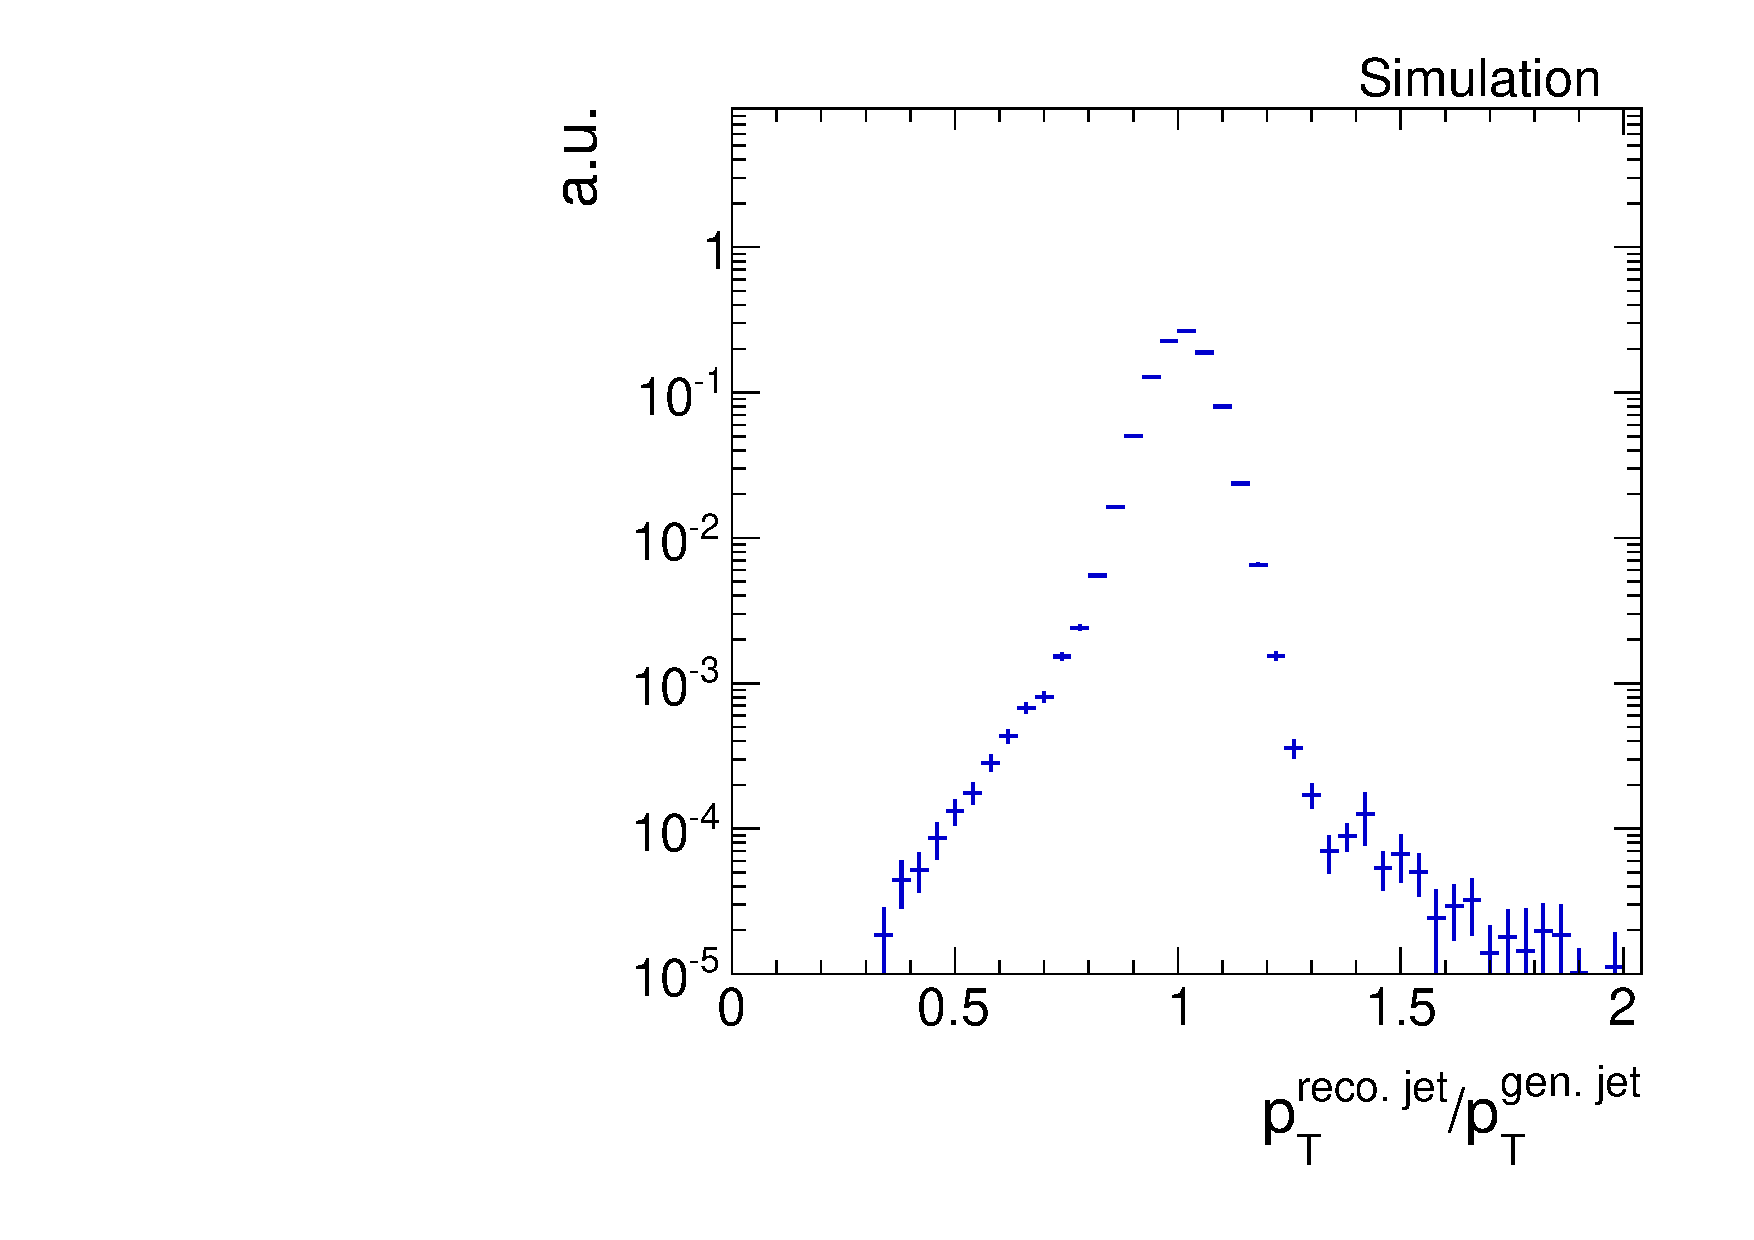
\includegraphics[width=0.49\textwidth]{figures/resolution/generalApproach/ExampleResponse.pdf}
      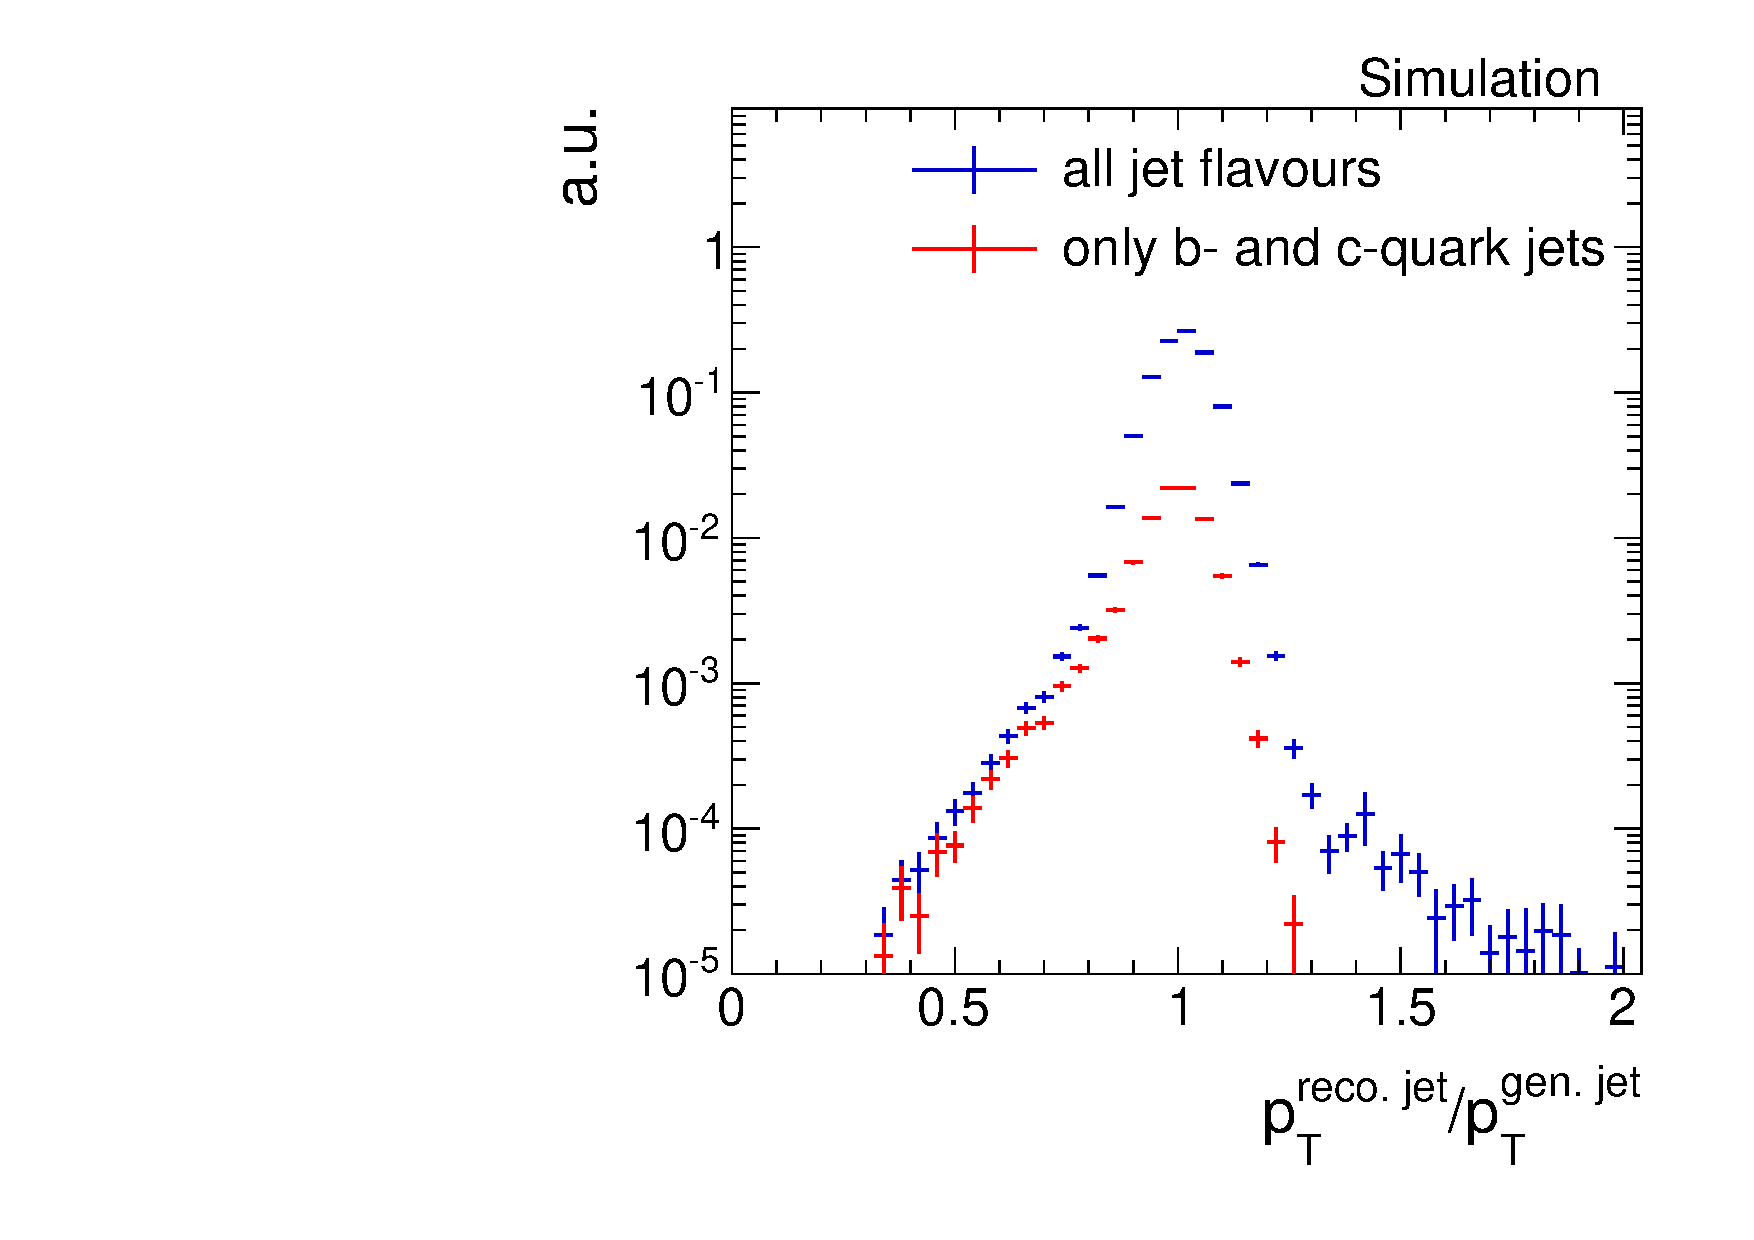
\includegraphics[width=0.49\textwidth]{figures/resolution/generalApproach/intrinsicExampleContributionofBCQuarks.pdf}
  \caption{Left:  Normalised number of events over \ptrecojet/\ptgenjet from a simulated \GAMJET sample. 
           Right: The response distribution containing all jet flavours (blue) and the contribution by c- and b-quark jets (red). }  
  \label{res:fig:TypicalResponse}
\end{figure}
Some instrumental effects, such as a non-linear response of the calorimeter, inhomogeneities of the detector material and electronic noise can contribute to both tails, 
others, like dead calorimeter channels only contribute to the left tail~\cite{bib:Matthias_Thesis}. 



%Figure~\ref{res:fig:TypicalResponse} shows a response distribution for jets in the barrel region.
In order to avoid the coverage of non-Gaussian tails, the resolution is determined using only the core of the response distribution.
The resolution is thus defined as the standard deviation of the 99\% truncated response histogram divided by the mean:
\begin{equation*}\label{res:eq:resolutionFormula}
\jer = \frac{\sigma_{99\%}}{\mu_{99\%}}.
\end{equation*}
The division by the mean aims at making the resolution independent of the absolute scale (= mean) of the response distribution.
It is done because response distributions with a scale smaller than one are typically narrower while distributions with scales larger than one are broader.
%However, since the scale is very close to one, this is only a tiny effect.

The determination of the 99\% range of the histogram is done in several steps. 
First the mean of the core is found via a Gaussian fit to the histogram in a 2$\sigma$ range\footnote{The 2$\sigma$ range is defined as the range [$\mu - 2\sigma$,$\mu + 2\sigma$].}. 
This procedure is done in three iteration steps.
Then, a symmetric interval around this mean is determined with its integral equal to 99\% of the integral of the full histogram. 

As noted earlier, in simulated data, the response distribution can be evaluated by the reconstructed over generator-level jet transverse momentum.
A determination of the resolution in real data, however, has to rely on a different approach.\\



The main idea of a resolution measurement using \GAMJET events is based on the transverse-momentum balance of the \GAMJET system and the excellent electromagnetic calorimeter resolution.

In Fig~\ref{res:fig:FeynmanDiagrams}, all tree-level processes contributing to an event topology with one photon and one jet in the final state are depicted. 
\begin{figure}[b]
  \centering
      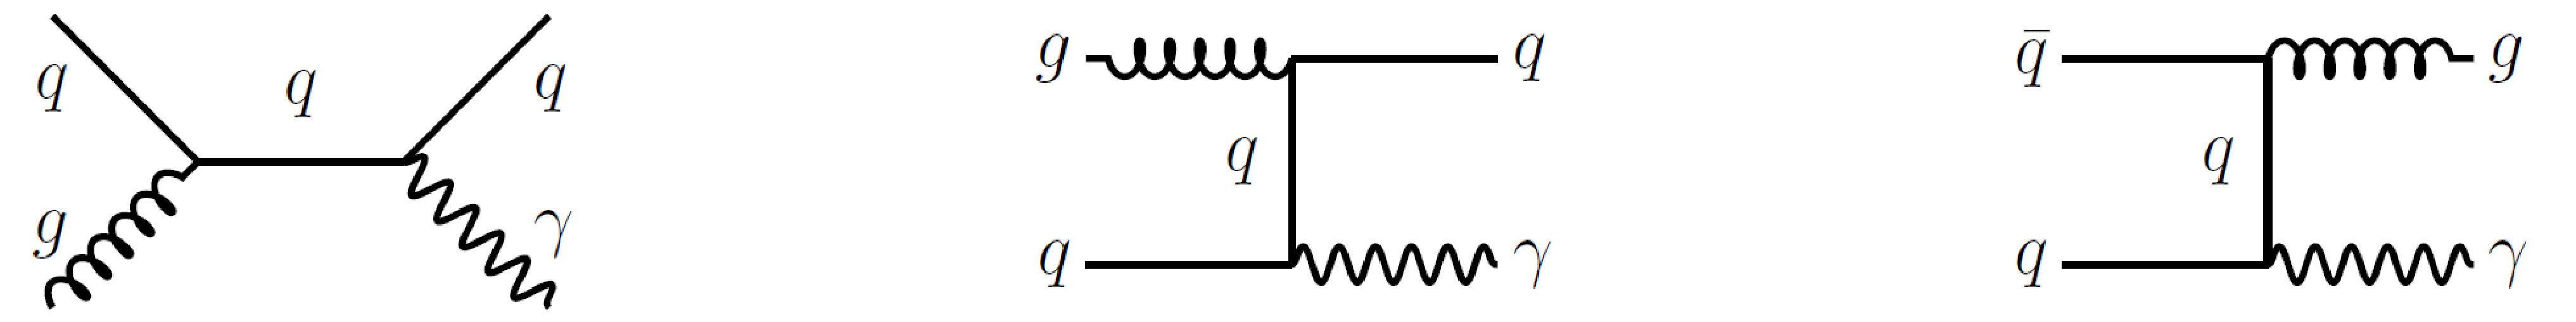
\includegraphics[width=0.99\textwidth]{figures/resolution/generalApproach/FeynmanDiagram.pdf}
  \caption{Tree-level Feynman diagrams of processes in $pp$-collisions with one photon and one jet in the final state.}  
  \label{res:fig:FeynmanDiagrams}
\end{figure}
Due to momentum conservation, the jet and the photon are back to back in the transverse plane, and therefore, $\ptvec^{\,\,\gamma} = -\ptvec^{\,\,\text{jet}}$. 
Because of the high resolution of the electromagnetic calorimeter, photon energies can be measured very accurately (with an resolution between 1.4\% and 3.8\% in the barrel region for $\sqrt{s}=8\tev$ data~\cite{bib:CMS:PhotonIdentification_8TeV}).
Thus, they can serve as an excellent estimator for the true jet transverse-momentum.


Unfortunately, such clean events are very rare processes, and usually, the momentum balance is spoiled by further jet activity from initial and final state radiation (see Fig.~\ref{res:fig:FeynmanDiagramsWithRadiation}). 
In order to select events that are balanced to a large extent, a lower bound on the angular distance in the transverse plane between the photon and the jet with the highest transverse momentum (leading jet) is required: $\Delta\Phi \left(\text{\nth{1}\,jet,\,} \gamma \right)>2.95\,\unit{rad}$. 

Additionally, the variable 
\begin{equation*}
\label{res:eq:alphaDef}
\alpha \doteq \frac{\ptsecondrecojet}{\ptgamma}
\end{equation*} 
is defined as a measure of further jet activity in an event. 
It is, however, not sufficient to require only an upper bound on $\alpha$. 
Instead, the jet transverse-momentum resolution is measured in bins of $\alpha$ with max($\alpha$) = 0.2, 
and the extrapolated value to zero further jet momentum at $\alpha=0$ is taken as the measured resolution of the jet \pt. % in the absence of further jets.
\begin{figure}[t]
  \centering
      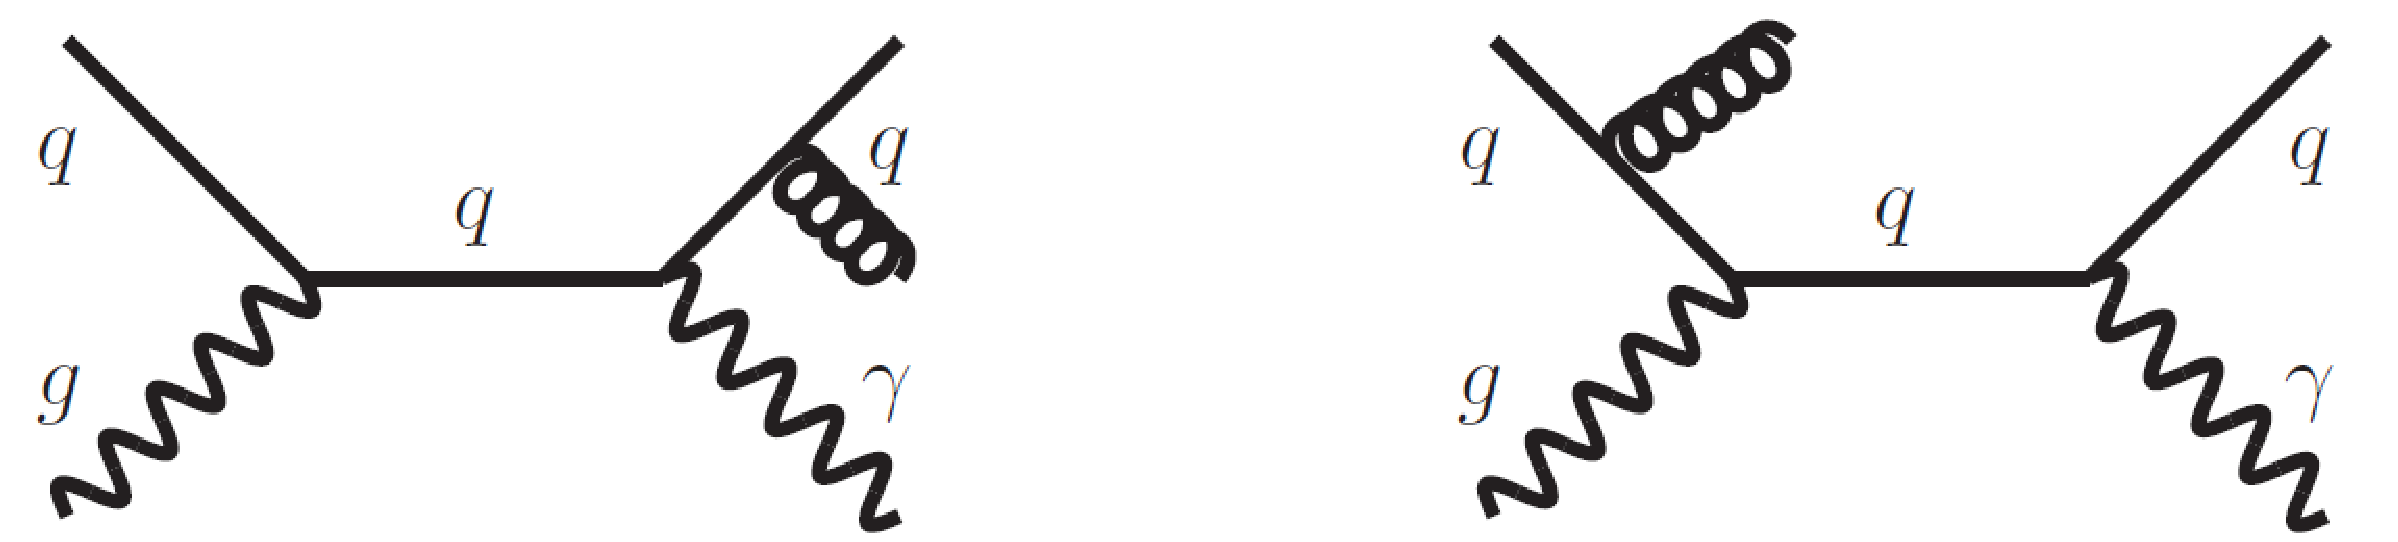
\includegraphics[width=0.60\textwidth]{figures/resolution/generalApproach/FeynmanDiagramsWithRadiation.pdf}
  \caption{Tree-level Feynman diagrams with final (left) and initial (right) state radiation.}  
  \label{res:fig:FeynmanDiagramsWithRadiation}
\end{figure}

More formally, measuring the transverse momentum of the photon instead of taking the generator-level jet \pt leads to the fact that the measured resolution consists of two parts
\begin{equation*}\label{res:eq:splitting}
\underbrace{\frac{\ptrecojet}{\ptgamma}}_{\text{measured}} = \underbrace{\frac{\ptrecojet}{\ptgenjet}}_{\text{intrinsic}} \oplus \underbrace{\frac{\ptgenjet}{\ptgamma}}_{\text{imbalance}}.
\end{equation*}
The intrinsic part is the resolution of interest which is independent of further jets in the event, whereas the imbalance is an artifact of further jet activity and is strongly dependent on $\alpha$.


To account for differences in the jet transverse-momentum resolution for different true jet \pt and different jet pseudorapidity regions, the measurement of the resolution is done in \ptgamma bins and bins of $|\eta|$ of the leading jet.

As noted before, the resolution measurement is important to correct the resolution measured in simulation to the resolution measured in data.
Therefore, the measurement of the jet transverse-momentum resolution is conducted on real and on simulated events and data-to-simulation resolution scale factors (\rhores) are determined
%%%%%%%%%%%%%%%%%%%%%%%%%%%%%%%%%%%%%%%%%%%%%%%%%%%%%%%%%%%%%%%%%%%%%%%%%%%%%%%%%%%%%%%%%%%%%%%%%%%%%%%%%%%%%%%%%%%%%%%%%%%%%%%%%%%%%%%%%%%%%%%%%%%%%%%%%%%%%%%%%%%%%%%%%%%%%%%%%%%%%%%%%%%%%%%%%%%%%%%%%%%%%%%%%%%%%%%%%%%%%%%%%%%
%%%%%%%%%%%%%%%%%%%%%%%%%%%%%%%%%%%%%%%%%%%%%%%%%%%%%%%%%%%%%%%%%%%%%%%%%%%%%%%%%%%%%%%%%%%%%%%%%%%%%%%%%%%%%%%%%%%%%%%%%%%%%%%%%%%%%%%%%%%%%%%%%%%%%%%%%%%%%%%%%%%%%%%%%%%%%%%%%%%%%%%%%%%%%%%%%%%%%%%%%%%%%%%%%%%%%%%%%%%%%%%%%%%
%%%%%%%%%%%%%%%%%%%%%%%%%%%%%%%%%%%%%%%%%%%%%%%%%%%%%%%%%%%%%%%%%%%%%%%%%%%%%%%%%%%%%%%%%%%%%%%%%%%%%%%%%%%%%%%%%%%%%%%%%%%%%%%%%%%%%%%%%%%%%%%%%%%%%%%%%%%%%%%%%%%%%%%%%%%%%%%%%%%%%%%%%%%%%%%%%%%%%%%%%%%%%%%%%%%%%%%%%%%%%%%%%%%
\FloatBarrier
\chapter{Datasets and event selection}

The measurement of the jet transverse-momentum resolution is carried out with \GAMJET data recorded during the year 2012 at a centre-of-mass energy of $\sqrt{s}=8\tev$ at the CMS experiment.
The datasets and triggers that are exploited for this measurement are introduced in the following Section~\ref{res:sec:DatasetsAndTriggers}.
The measured resolution in data is compared to the resolution in simulated samples. These are introduced in Section~\ref{res:sec:SimulatedSamples}.
In order to select \GAMJET events that are well suited for the resolution measurement, an event selection is applied on top.
This event selection is described in Section~\ref{res:sec:EventSelection}.

\section{Datasets and triggers}
\label{res:sec:DatasetsAndTriggers}
This analysis exploits several triggers which were active during the year 2012 at the CMS experiment.
Because of the high production cross section of \GAMJET events, especially for low photon \pt, almost all of these triggers were highly prescaled, \ie only a fraction of events were actually recorded when the triggers fired.
All triggers that are utilised in this measurement are listed in Table~\ref{res:tab:triggers} together with their recorded luminosity.
\renewcommand{\arraystretch}{1.5}
\begin{table}[!b]
\centering
\caption{Single-photon triggers together with the recorded luminosity taking the prescales of the triggers into consideration.}
\label{res:tab:triggers}
\makebox[0.99\textwidth]{
\begin{tabular}{lr}
\multicolumn{2}{c}{} \\
\toprule
Trigger                       & Integrated luminosity [\fbinv]   \\
\midrule
%HLT\_Photon20\_CaloIdVL\_IsoL & 0.0008\\
HLT\_Photon30\_CaloIdVL\_IsoL & 0.0029\\
HLT\_Photon50\_CaloIdVL\_IsoL & 0.0607\\
HLT\_Photon75\_CaloIdVL\_IsoL & 0.123\\
HLT\_Photon90\_CaloIdVL\_IsoL & 0.373\\
HLT\_Photon135\               & 13.77\\
HLT\_Photon150\               & 19.71\\
\bottomrule
\multicolumn{2}{c}{} \\
\end{tabular}}
\end{table}  
On level one (L1), the triggers rely on single-photon triggers, such as L1SingleEG12 and L1SingleEG30.
The L1 triggers require at least one photon that is above a certain \pt threshold, \eg 12\gev or 30\gev.
The high-level triggers require a photon with a certain \pt (as indicated in the name) and, in case of thresholds below 135\gev, additional quality and isolation criteria. 
All triggers with threshold below 150\gev were prescaled.

The events that are selected by the above mentioned triggers are contained in the datasets listed in Table~\ref{res:tab:datasets}.
\renewcommand{\arraystretch}{1.5}
\begin{table}[!hbt]
\centering
\caption{Single-photon data samples used for the resolution measurement with the contained integrated luminosity.}
\label{res:tab:datasets}
\makebox[0.99\textwidth]{
\begin{tabular}{l r}
\multicolumn{2}{c}{} \\
\toprule
Dataset                                          & Integrated luminosity [\fbinv]   \\
\midrule
 /Photon/Run2012A-22Jan2013-v1/AOD               &  0.876   \\
 /SinglePhoton/Run2012B-22Jan2013-v1/AOD         &  4.412  \\
 /SinglePhoton/Run2012C-22Jan2013-v1/AOD         &  7.055  \\
 /SinglePhotonParked/Run2012D-22Jan2013-v1/AOD   &  7.354  \\ 
\bottomrule
\multicolumn{2}{c}{} \\
\end{tabular}}
\end{table}  

\section{Simulated samples}
\label{res:sec:SimulatedSamples}

In order to compare the measured resolution in data to the resolution in simulation, a single-photon sample simulated with \pythiaSix is used.
This sample is generated flat in the photon \pt to have a good statistical precision also for the high photon \pt region.
In order to recover a physical \pt spectrum, all simulated events are reweighted.
Figure~\ref{res:fig:PhotonPtSpectrum} shows the photon \pt spectrum in simulation before and after the reweighting. 

All simulated samples come with a pileup scenario which does not necessarily match the pileup scenario in data. 
To match the measured distribution of primary vertices, the events are weighted according to their number of primary vertices. 
Because almost all of the used triggers were differently prescaled over time, the distributions of primary vertices differ among the sets of events recorded by each trigger.
Thus, the reweighting has to be done separately for each trigger.
A comparison between the number of primary vertices in real data and simulation for all triggers can be found in Appendix~\ref{res:app:pileup}.
\begin{figure}[ht]
  \centering
      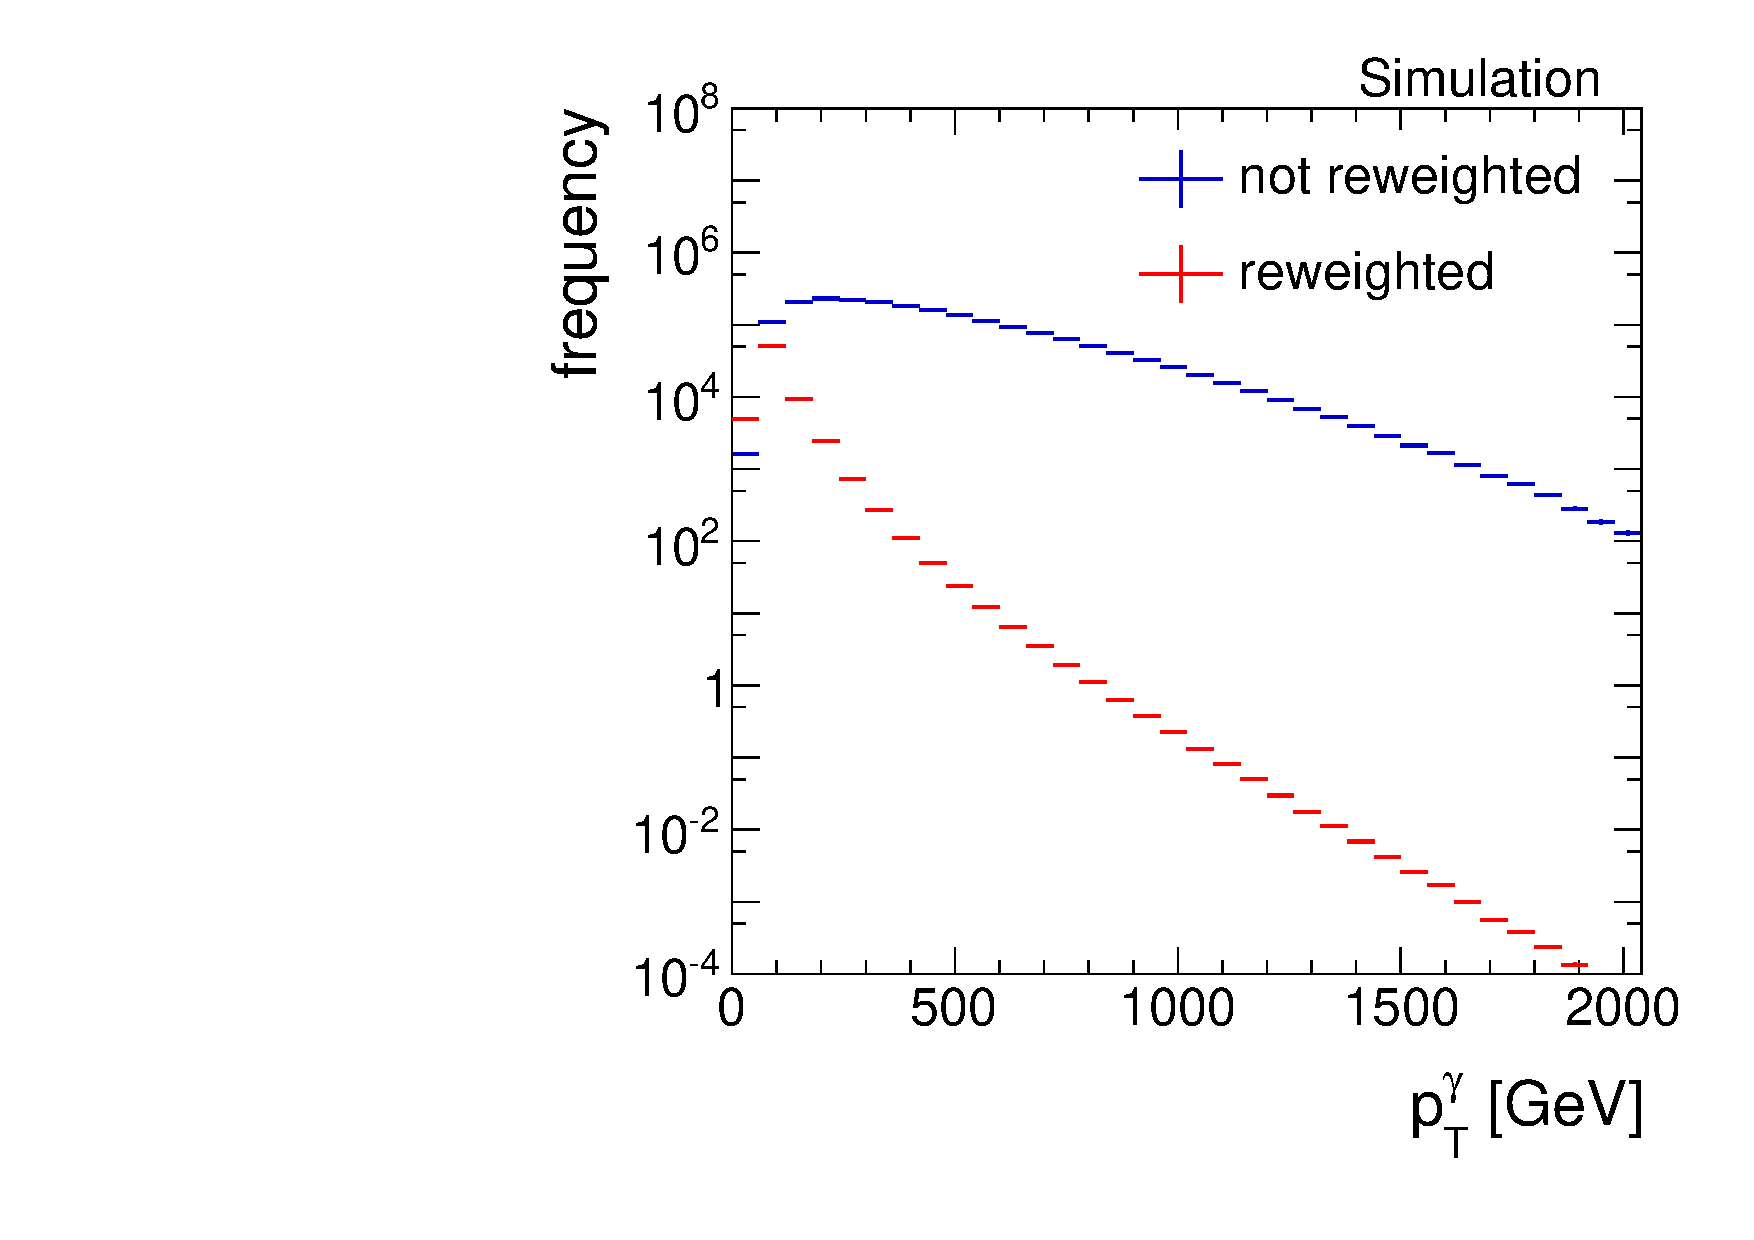
\includegraphics[width=0.49\textwidth]{figures/resolution/eventSelection/PhotonPtComparison_reweighted.pdf} 
  \caption{The photon \pt spectrum of the \pythiaSix simulated single-photon sample before (blue) and after (red) reweighting.}  
  \label{res:fig:PhotonPtSpectrum}
\end{figure}


\section{Event selection}
\label{res:sec:EventSelection}
Events are reconstructed with the particle-flow reconstruction algorithm, which uses information of all detector components to reconstruct individual particles~\cite{CMS-PAS-PFT-09-001}.
In the following, the selection of well reconstructed jets and photons will be explained as well as the event selection of \GAMJET events.

\subsection{Jet selection}
Particles belonging to a jet are clustered with the Anti-k$_{\text{t}}$ jet clustering algorithm with a radius of R=0.5~\cite{Cacciari:2008gp}.
Furthermore, all reconstructed jets undergo a so-called ``charged hadron subtraction'' (CHS) which removes hadrons that are likely caused by pileup events.

To select clean \GAMJET events, it is required that the leading jet meets the ``tight ID'' selection requirements for jets~\cite{bib:JetIDRecommendation_7TeV,bib:AN:JetId_8TeV}.
The tight ID selection ensures a selection efficiency of around 99\% and a noise rejection efficiency of 99.98\%~\cite{bib:JetIDRecommendation_7TeV}.
It comprises the following selection criteria:
\begin{itemize}
 \item Neutral hadron fraction $<$ 0.90
 \item Neutral electromagnetic fraction $<$ 0.90
 \item Number of constituents $>$ 1
\end{itemize}
 And for jets in the pseudorapidity range $|\eta| < 2.4 $ :
\begin{itemize}
 \item Charged hadron fraction $>$ 0
 \item Charged hadron multiplicity $>$ 0
 \item Charged electromagnetic fraction $<$ 0.99.
\end{itemize}

To mitigate effects from pileup, an additional transverse-momentum requirement is imposed:
\begin{itemize}
\item $\ptfirstjet,\ptsecondjet>10\gev$.
\end{itemize}

\subsection{Photon selection}
\label{subsec:PhotonSelection}
Concerning the photon, a maximum pseudorapidity of the photon of $|\eta^{\gamma}| < 1.3$ is demanded to exploit the high resolution of the ECAL in the barrel region.

Furthermore, the resolution is determined for different ranges in photon \pt to avoid mixing of different prescales of the various triggers. 
In Table~\ref{res:tab:PhotonPtBins} the applied binning is shown with the respective triggers contributing to each $\pt^{\gamma}$ bin.
\renewcommand{\arraystretch}{1.5}
\begin{table}[htb]
\centering
\caption{Photon \pt bins and corresponding triggers.}
\label{res:tab:PhotonPtBins}
\makebox[0.99\textwidth]{
\begin{tabular}{ll}
\multicolumn{2}{c}{} \\
\toprule
$\pt^{\gamma}$-bins           & Trigger         \\
\midrule
%22\gev       &  HLT\_Photon20\_CaloIdVL\_IsoL\_v* \\
36-60\gev    & HLT\_Photon30\_CaloIdVL\_IsoL\_v* \\
60-88\gev    & HLT\_Photon50\_CaloIdVL\_IsoL\_v* \\
88-105\gev    & HLT\_Photon75\_CaloIdVL\_IsoL\_v* \\
105-149\gev   & HLT\_Photon90\_CaloIdVL\_IsoL\_v* \\
149-165\gev \qquad\qquad   & HLT\_Photon135\_v*                \\
165-$\infty$\gev   & HLT\_Photon150\_v*                \\
\bottomrule
\multicolumn{2}{c}{} \\
\end{tabular}}
\end{table}

QCD-multijet events constitute an important background to \GAMJET events: A photon can be faked by a $\pi^{0}$ decaying into two close-by photons. 
Therefore, a very clean selection of the photons is necessary to suppress this background.
The following variables are used (see~\cite{CMS-PAS-EGM-10-006} for further explanation of the variables):

\begin{itemize}
 \item $\frac{\textbf{H}}{\textbf{E}}$ : The ratio of the measured energy in the hadronic calorimeter over the energy measured in the electromagnetic calorimeter. 
                                                    For photons, this is supposed to be very small as they deposit their energy predominantly in the ECAL.
 \item $\mathbold{\sigma_{i\eta i \eta}}$: The energy weighted spatial width of the photon energy deposition. The electromagnetic shower of a photon has a small lateral size 
                                           resulting in small $\sigma_{i\eta i \eta}$ for prompt photons while showers from fake photons, \eg $\pi^{0} \rightarrow \gamma \gamma$
                                           have a larger lateral size.
 \item \textbf{Jurassic ECAL isolation}: This isolation criterion uses the information of reconstructed hits ``RecHits'' (coming from the local reconstruction of the digital signals) 
                                         in a cone around the photon supercluster of R=0.4. Those are summed up and an upper criterion is identified to discriminate against 
                                         background which is typically spatially broader.  
 \item \textbf{Tower-based HCAL isolation}: The isolation criterion requires the energy deposited in all HCAL towers around the photon in cone of R=0.4 to be small compared to the 
                                            photon's energy. 
 \item \textbf{Hollow cone track isolation}: Requires absence of high-energetic tracks around the photon.
 \item \textbf{Pixel seed veto}: In order to reduce the background from electrons and positrons, the absence of a pixel-seed in the pixel tracker along the photons 
                                 trajectory is required.
\end{itemize}

The upper bounds that are set on these observables can be found in Table~\ref{res:tab:PhotonIsolation}. 
\renewcommand{\arraystretch}{1.5}
\begin{table}[htb]
\centering
\caption{Upper bounds for all photon isolation criteria in the barrel $\left( |\eta^{\gamma}|<1.4442 \right)$.}
\label{res:tab:PhotonIsolation}
\makebox[0.99\textwidth]{
\begin{tabular}{lc}
\multicolumn{2}{c}{} \\
\toprule
                              & Barrel                          \\
\midrule
$\frac{\text{H}}{\text{E}}$   & $<$ 0.05                        \\
$\sigma_{i\eta i \eta}$           & $<$ 0.013                       \\
ECAL isolation                & $<4.2\gev + 0.0060 \cdot \pt^{\gamma}$   \\
HCAL isolation                & $<2.2\gev + 0.0025 \cdot \pt^{\gamma}$   \\
Track Isolation               & $<2.0\gev + 0.0010 \cdot \pt^{\gamma}$   \\
Pixel seed veto               & yes                              \\
\bottomrule
\multicolumn{2}{c}{} \\
\end{tabular}}
\end{table}
%\begin{table}[bt]
%\caption{Upper and lower bounds for all photon isolation criteria in the barrel $\left( |\eta^{\gamma}|<1.4442 \right)$ and endcap $\left(1.4442 <|\eta^{\gamma}|<2.5 \right)$ .}
%\renewcommand{\arraystretch}{1.5}
%\begin{center}
%\begin{tabular}{ l| c | c |}
%                              & Barrel                                  & Endcap                                  \\\hline
%$\frac{\text{H}}{\text{E}}$   & $<$ 0.05                                & $<$ 0.05                                \\\hline
%$\sigma_{i\eta i \eta}$       & $<$ 0.013                               & $<$ 0.03                                \\\hline
%ECAL isolation                & $<4.2 + 0.0060 \, \pt^{\gamma}$   & $<4.2 + 0.0060 \, \pt^{\gamma}$    \\\hline
%HCAL isolation                & $<2.2 + 0.0025 \, \pt^{\gamma}$   & $<2.2 + 0.0025 \, \pt^{\gamma}$   \\\hline
%Track Isolation               & $<2.0 + 0.0010 \, \pt^{\gamma}$   & $<2.0 + 0.0010 \, \pt^{\gamma}$    \\\hline
%Pixel seed veto               & yes                                     & yes                                     \\\hline
%\end{tabular}
%\end{center}
%\label{tab:PhotonIsolation}
%\end{table}

\subsection{Photon+jet event selection}
Besides the mentioned requirements concerning the objects' attributes, two further criteria related to the event topology are crucial for this analysis:\\
A lower threshold on $\Delta \Phi$ between the leading jet and the photon and a maximum value for $\alpha$
\begin{itemize}
 \item $\Delta \Phi \left(\text{\nth{1}\,jet},\,\gamma \right) > 2.95\,\unit{rad}$
 \item $\alpha = \frac{\ptsecondjet}{\ptgamma} < 0.20$.
\end{itemize}
These requirements are important to suppress events with too much further hadronic activity.
A summary of all selection criteria can be found in Appendix~\ref{res:app:eventselection}.\\

Finally, the leading jet pseudorapidity interval bounds need to be chosen in order to account for resolution differences in different detector regions.
This is done according to~\cite{bib:Matthias_Thesis} with the following binning
\begin{align*}
|\etafirstjet| = 0.0-0.5 && |\etafirstjet| = 1.1-1.7 \\
|\etafirstjet| = 0.5-1.1 && |\etafirstjet| = 1.7-2.3.
\end{align*}
The binning in the \ptgamma dimension is chosen according to the trigger thresholds for \mbox{$\ptgamma<165\gev$} and ensures sufficient statistical precision for \mbox{$\ptgamma>165\gev$}
\begin{align*}
\ptgamma &= 36 -60\gev     &  \ptgamma &= 149-165\gev   & \ptgamma &= 200-300\gev\\
\ptgamma &= 60 -88\gev     &  \ptgamma &= 165-176\gev  & \ptgamma &= 300-400\gev\\
\ptgamma &= 88 -105\gev    &  \ptgamma &= 176-200\gev  & \ptgamma &> 400\gev\\
\ptgamma &= 105-149\gev   \quad &  \ptgamma  &= 300-400\gev. \quad& \\
\end{align*}


%%%%%%%%%%%%%%%%%%%%%%%%%%%%%%%%%%%%%%%%%%%%%%%%%%%%%%%%%%%%%%%%%%%%%%%%%%%%%%%%%%%%%%%%%%%%%%%%%%%%%%%%%%%%%%%%%%%%%%%%%%%%%%%%%%%%%%%%%%%%%%%%%%%%%%%%%%%%%%%%%%%%%%%%%%%%%%%%%%%%%%%%%%%%%%%%%%%%%%%%%%%%%%%%%%%%%%%%%%%%%%%%%%%
%%%%%%%%%%%%%%%%%%%%%%%%%%%%%%%%%%%%%%%%%%%%%%%%%%%%%%%%%%%%%%%%%%%%%%%%%%%%%%%%%%%%%%%%%%%%%%%%%%%%%%%%%%%%%%%%%%%%%%%%%%%%%%%%%%%%%%%%%%%%%%%%%%%%%%%%%%%%%%%%%%%%%%%%%%%%%%%%%%%%%%%%%%%%%%%%%%%%%%%%%%%%%%%%%%%%%%%%%%%%%%%%%%%
%%%%%%%%%%%%%%%%%%%%%%%%%%%%%%%%%%%%%%%%%%%%%%%%%%%%%%%%%%%%%%%%%%%%%%%%%%%%%%%%%%%%%%%%%%%%%%%%%%%%%%%%%%%%%%%%%%%%%%%%%%%%%%%%%%%%%%%%%%%%%%%%%%%%%%%%%%%%%%%%%%%%%%%%%%%%%%%%%%%%%%%%%%%%%%%%%%%%%%%%%%%%%%%%%%%%%%%%%%%%%%%%%%%
\FloatBarrier
\chapter{Methodology of the measurement}
\label{res:ch:methodology}

The basic methodology of measuring the jet transverse-momentum resolution by exploiting the \pt balance in $\GAMJET$ events and extrapolating the result to small $\alpha$, that was already used in earlier analyses~\cite{bib:CMS:JERCPaper_2011,CMS:PAS:JETResolution_7TeV}, is extended in this measurement in order to explicitly account for the influence of the direction of additional jets on the jet transverse-momentum response.
% the case of parton radiation in different event hemispheres. FIXME

As already described in Chapter~\ref{res:ch:GeneralApproach}, the idea behind a resolution measurement with $\GAMJET$ events in real data is the usage of the photon \pt instead of the true jet \pt.
This results in a twofold contribution to the measured response, the intrinsic response and the imbalance:
\begin{equation}\label{eq:splittedResolution}
\underbrace{\frac{\ptrecojet}{\ptgamma}}_{\text{measured}} = \underbrace{\frac{\ptrecojet}{\ptgenjet}}_{\text{intrinsic}} \oplus \underbrace{\frac{\ptgenjet}{\ptgamma}}_{\text{imbalance}}.
\end{equation}
Taking the photon \pt as true jet \pt estimator instead of the generator-level jet \pt, and thus measuring the response defined as \ptrecojet/\ptgamma, results in a different shape of the response distribution compared to the intrinsic response (Fig.~\ref{fig:responseExamples}). 
\begin{figure}[b]
 \centering
     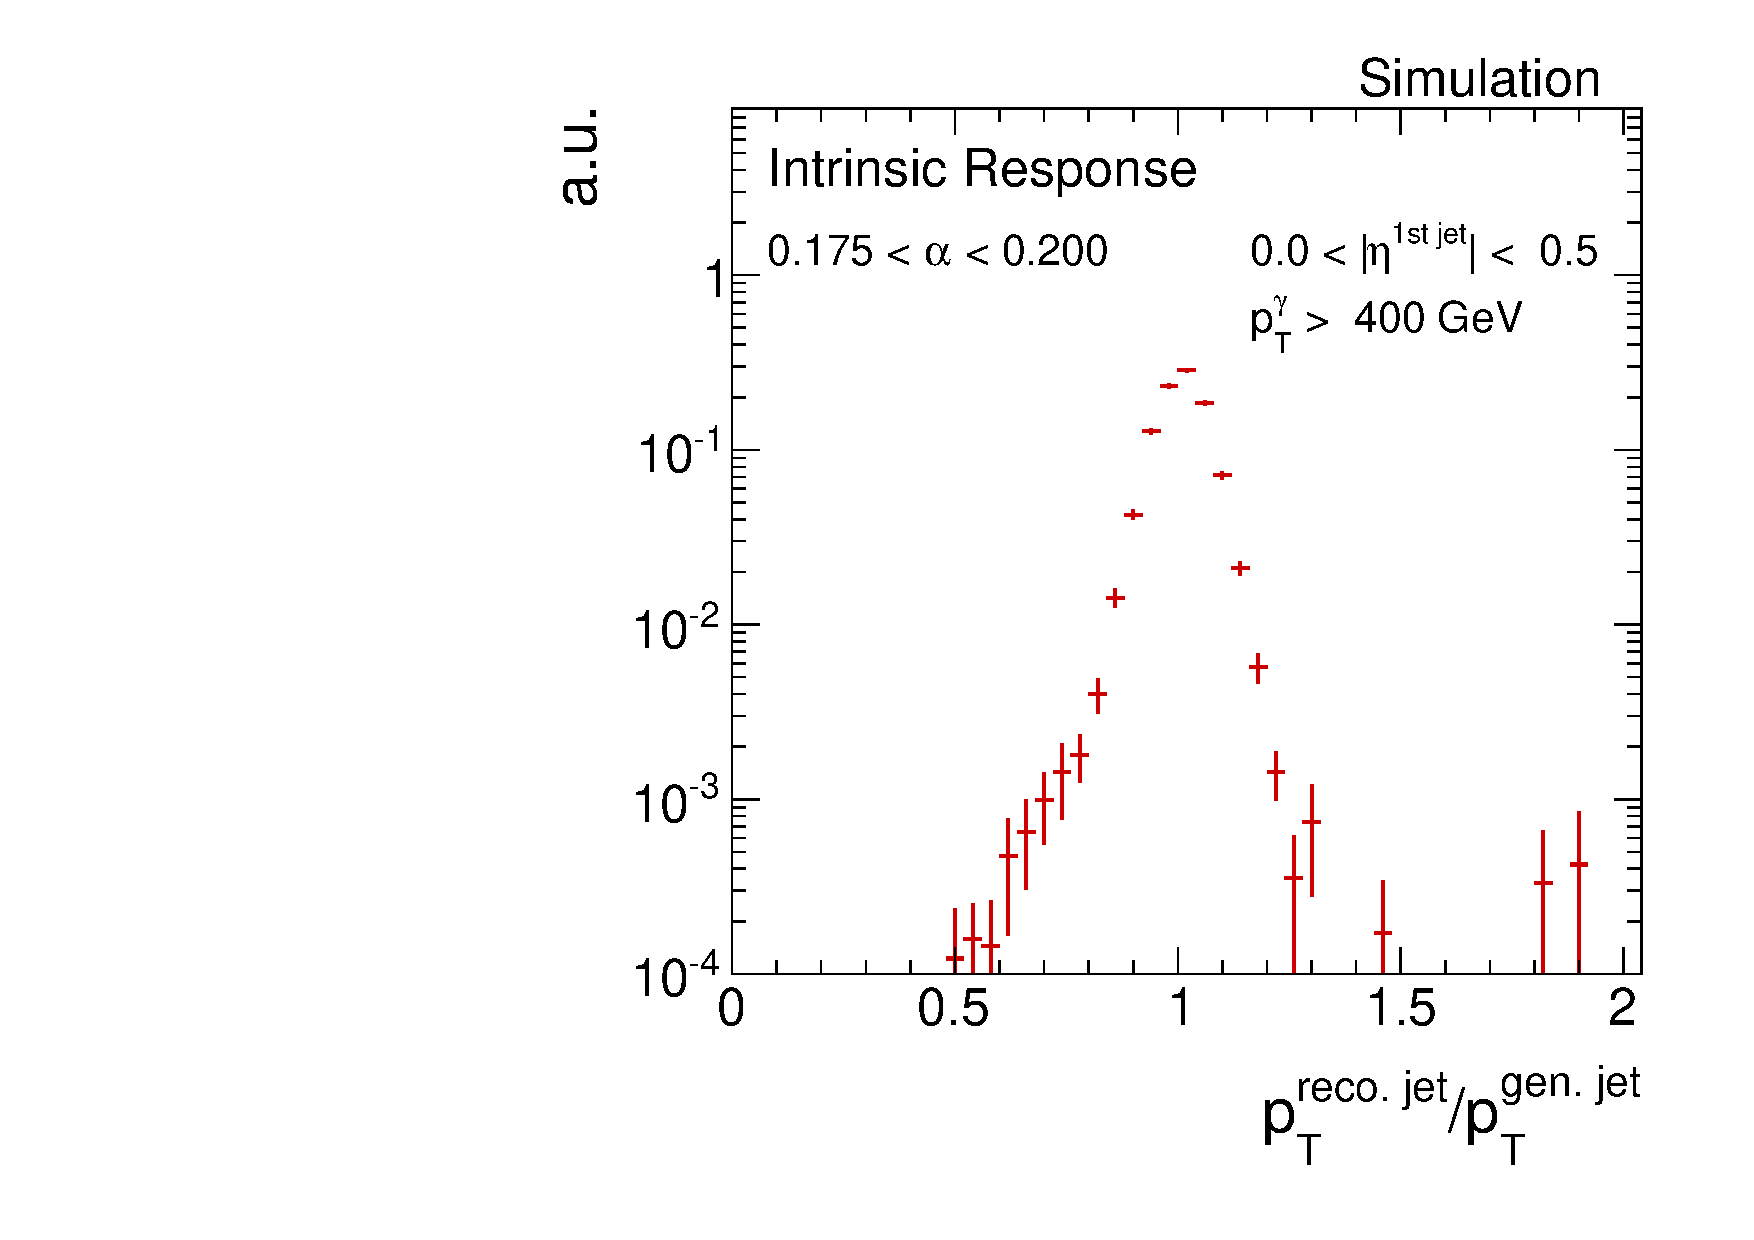
\includegraphics[width=0.49\textwidth]{figures/resolution/methodology/intrinsicResponse_6_alpha_bin.pdf}
     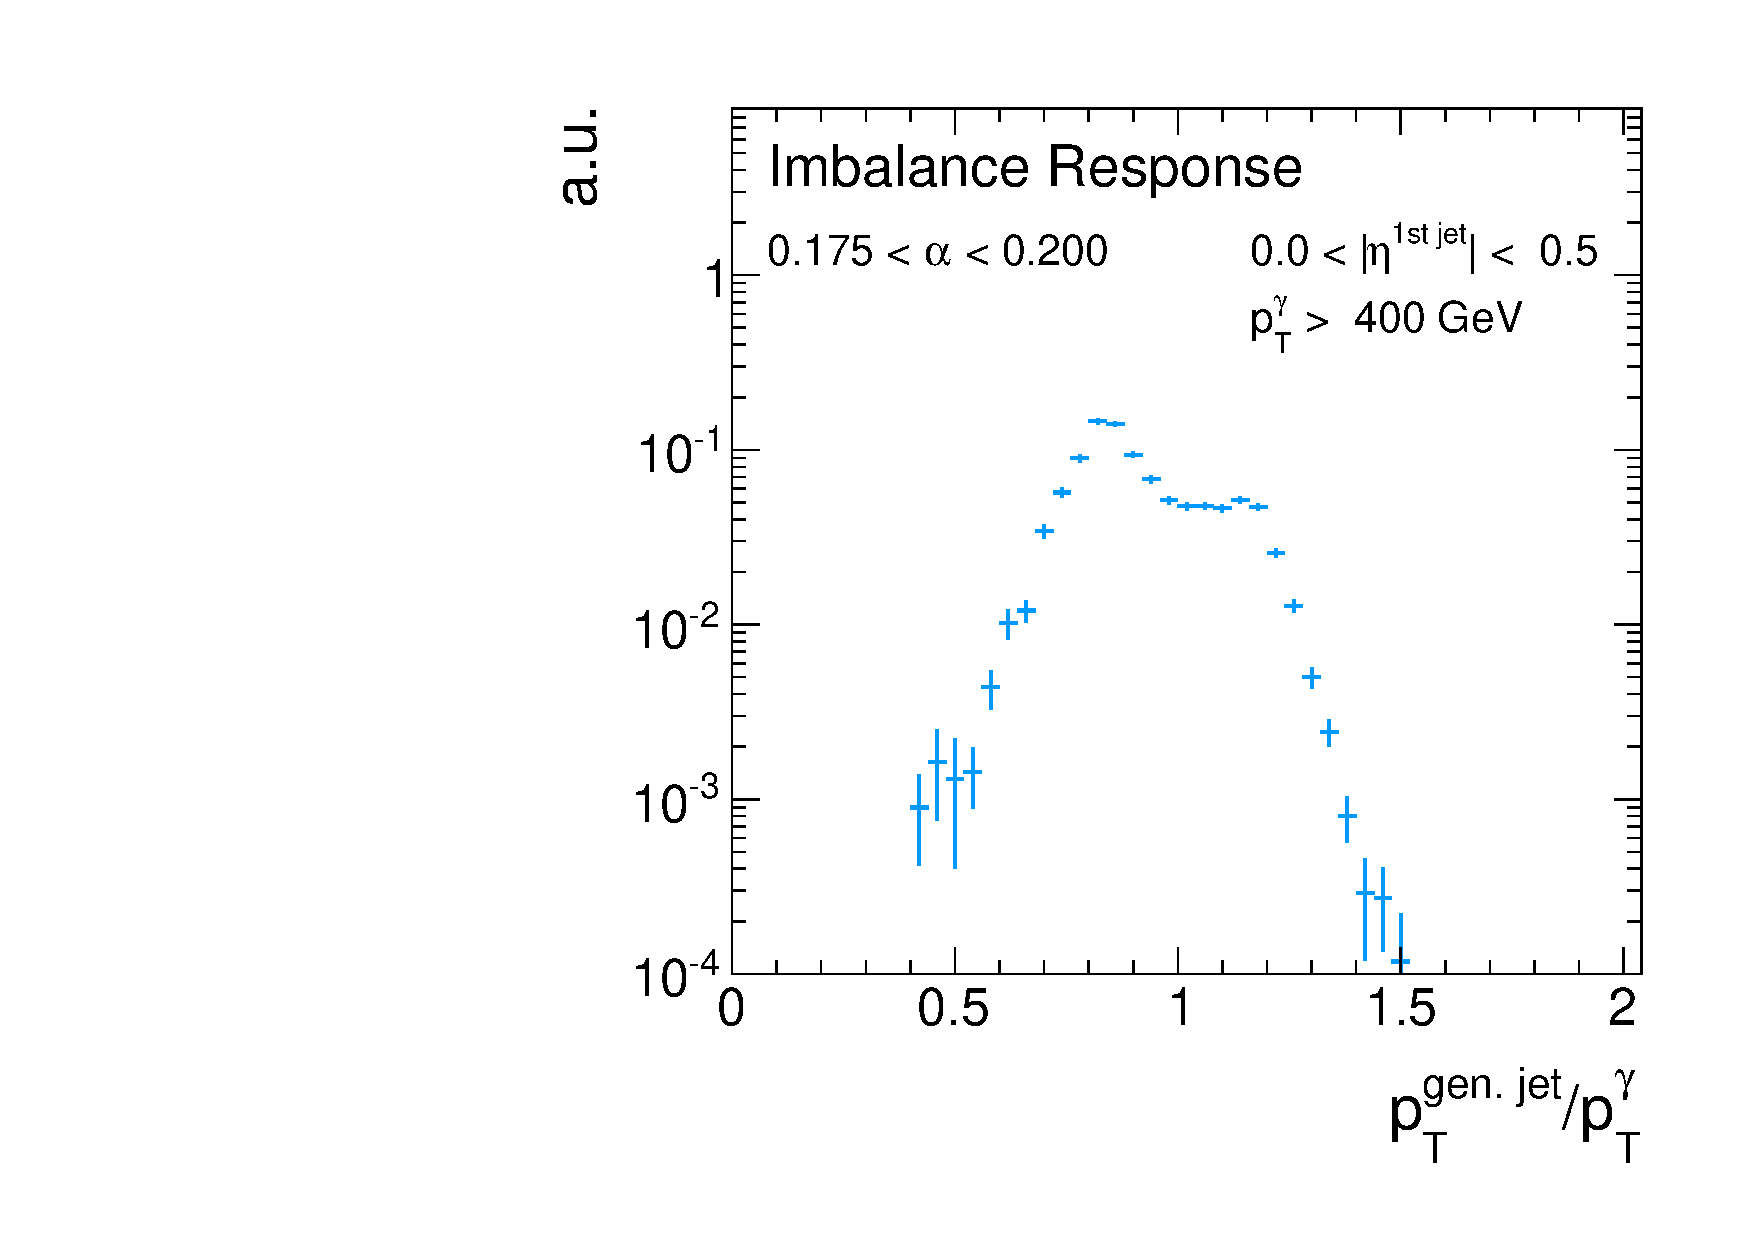
\includegraphics[width=0.49\textwidth]{figures/resolution/methodology/imbalanceResponse_6_alpha_bin.pdf}\\
     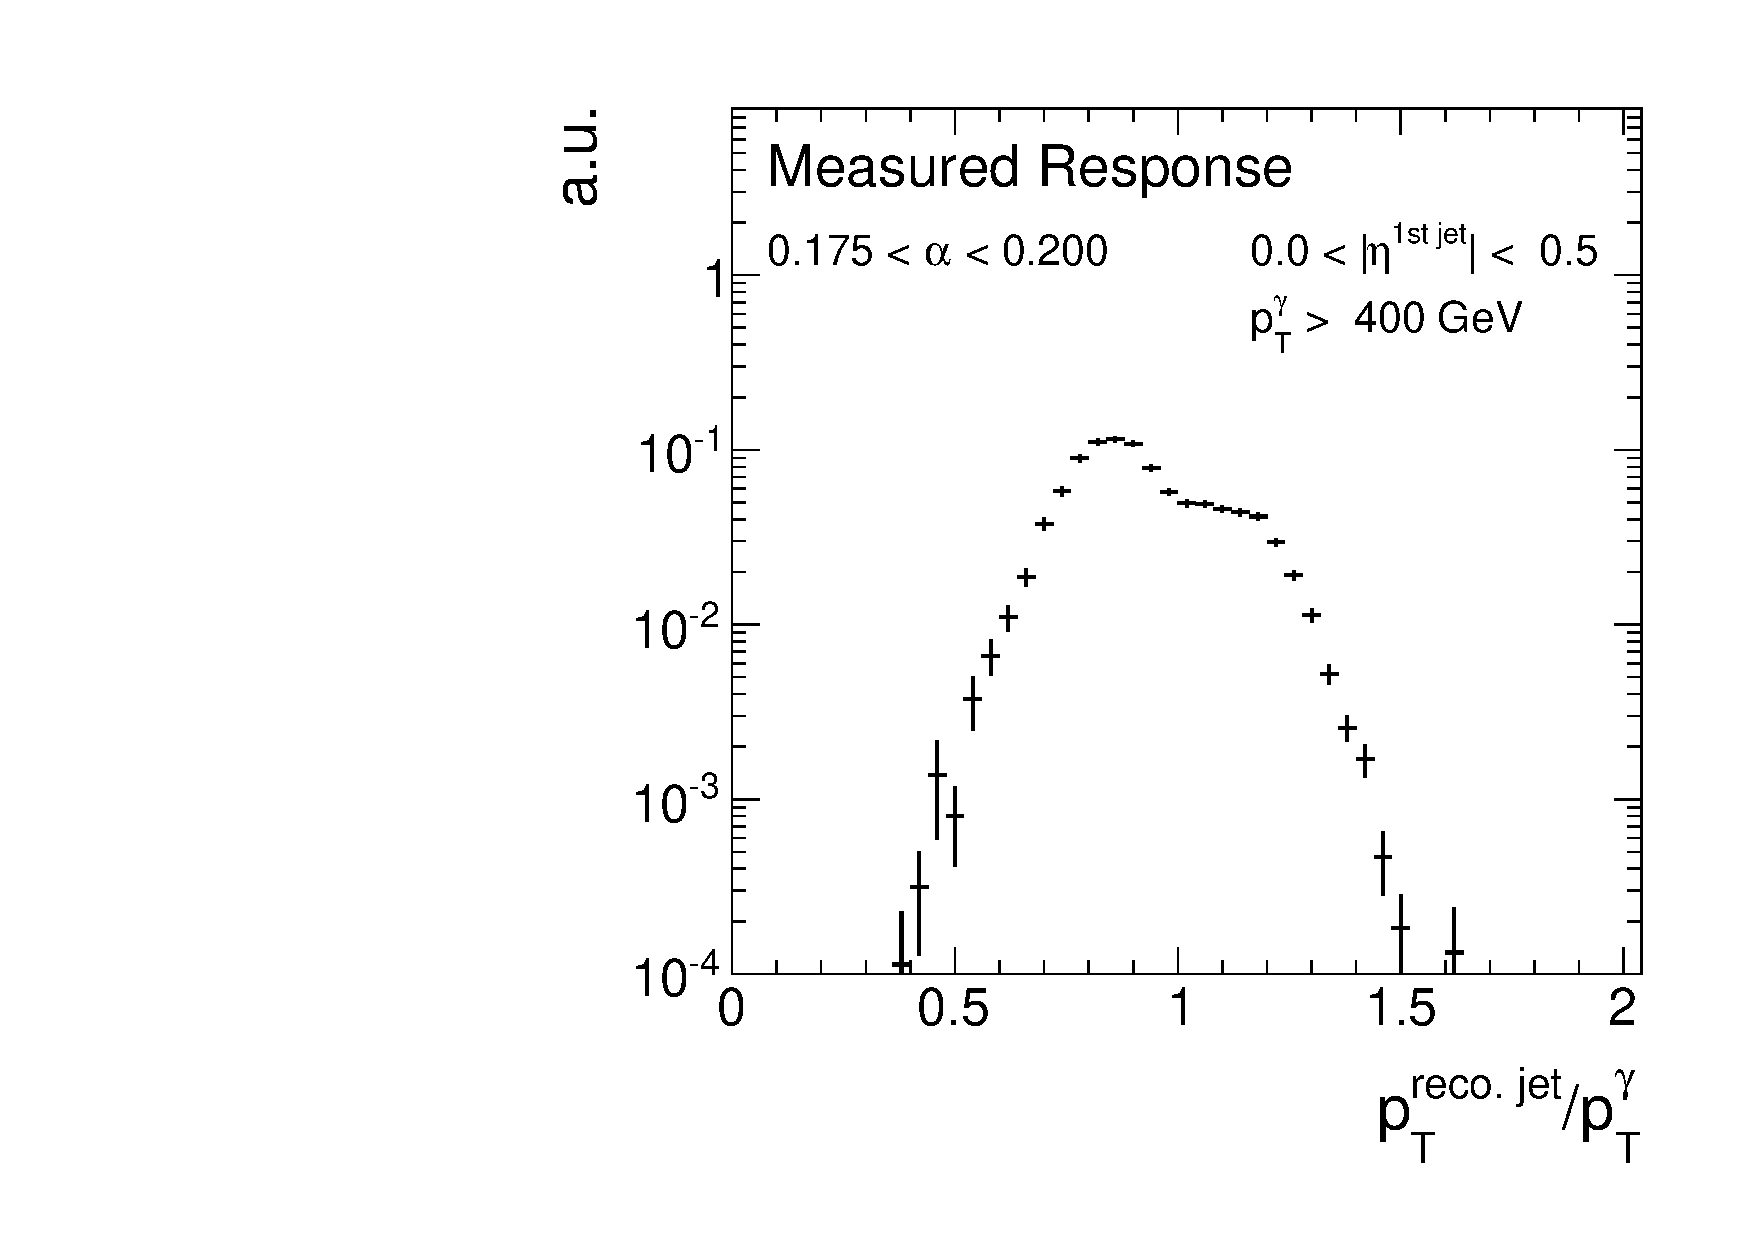
\includegraphics[width=0.49\textwidth]{figures/resolution/methodology/fullResponse_6_alpha_bin.pdf}
  \caption{The two different contributions, intrinsic (top left) and imbalance (top right), to the measured response (bottom) (cf. Eq.~\eqref{eq:splittedResolution}) in simulated events.}  
 \label{fig:responseExamples}
\end{figure}
The clear difference between the intrinsic response and the imbalance is the double peak structure of the latter one. The measured response is a convolution of the two
contributions, where the double peak is consequentially less pronounced.

The occurrence of two peaks is caused by the hard selection in $\Delta \Phi$ which forces the second jet to be either close to the photon or close to the leading jet due to \pt conservation. 
An energetic second jet perpendicular to the leading jet-photon axis would require a balancing third jet for \pt conservation.
This is very unlikely due to the decreasing probability of high jet multiplicities in QCD-multijet events.
Events can thus be distinguished by the relative direction of the second jet (see Fig.~\ref{fig:sketch} for a schematic sketch), with a hemisphere definition of
\begin{equation}\label{eq:HemisphereDefinition}
\begin{aligned}
  &\text{Second jet in \nth{1} jet hemisphere:}  \qquad  && \Delta \Phi \left( \text{\nth{1}\,jet,\,\nth{2} jet} \right) < \Delta \Phi \left( \gamma \text{,\,\nth{2}\,jet} \right) , \\
  &\text{Second jet in photon hemisphere:}        && \text{else}.\\
\end{aligned}
\end{equation}
%A schematic sketch of events with a second jet in the photon or leading jet hemisphere can be found in Fig.~\ref{fig:sketch}.
\begin{figure}[!b]
 \centering
 \vspace{30pt}
     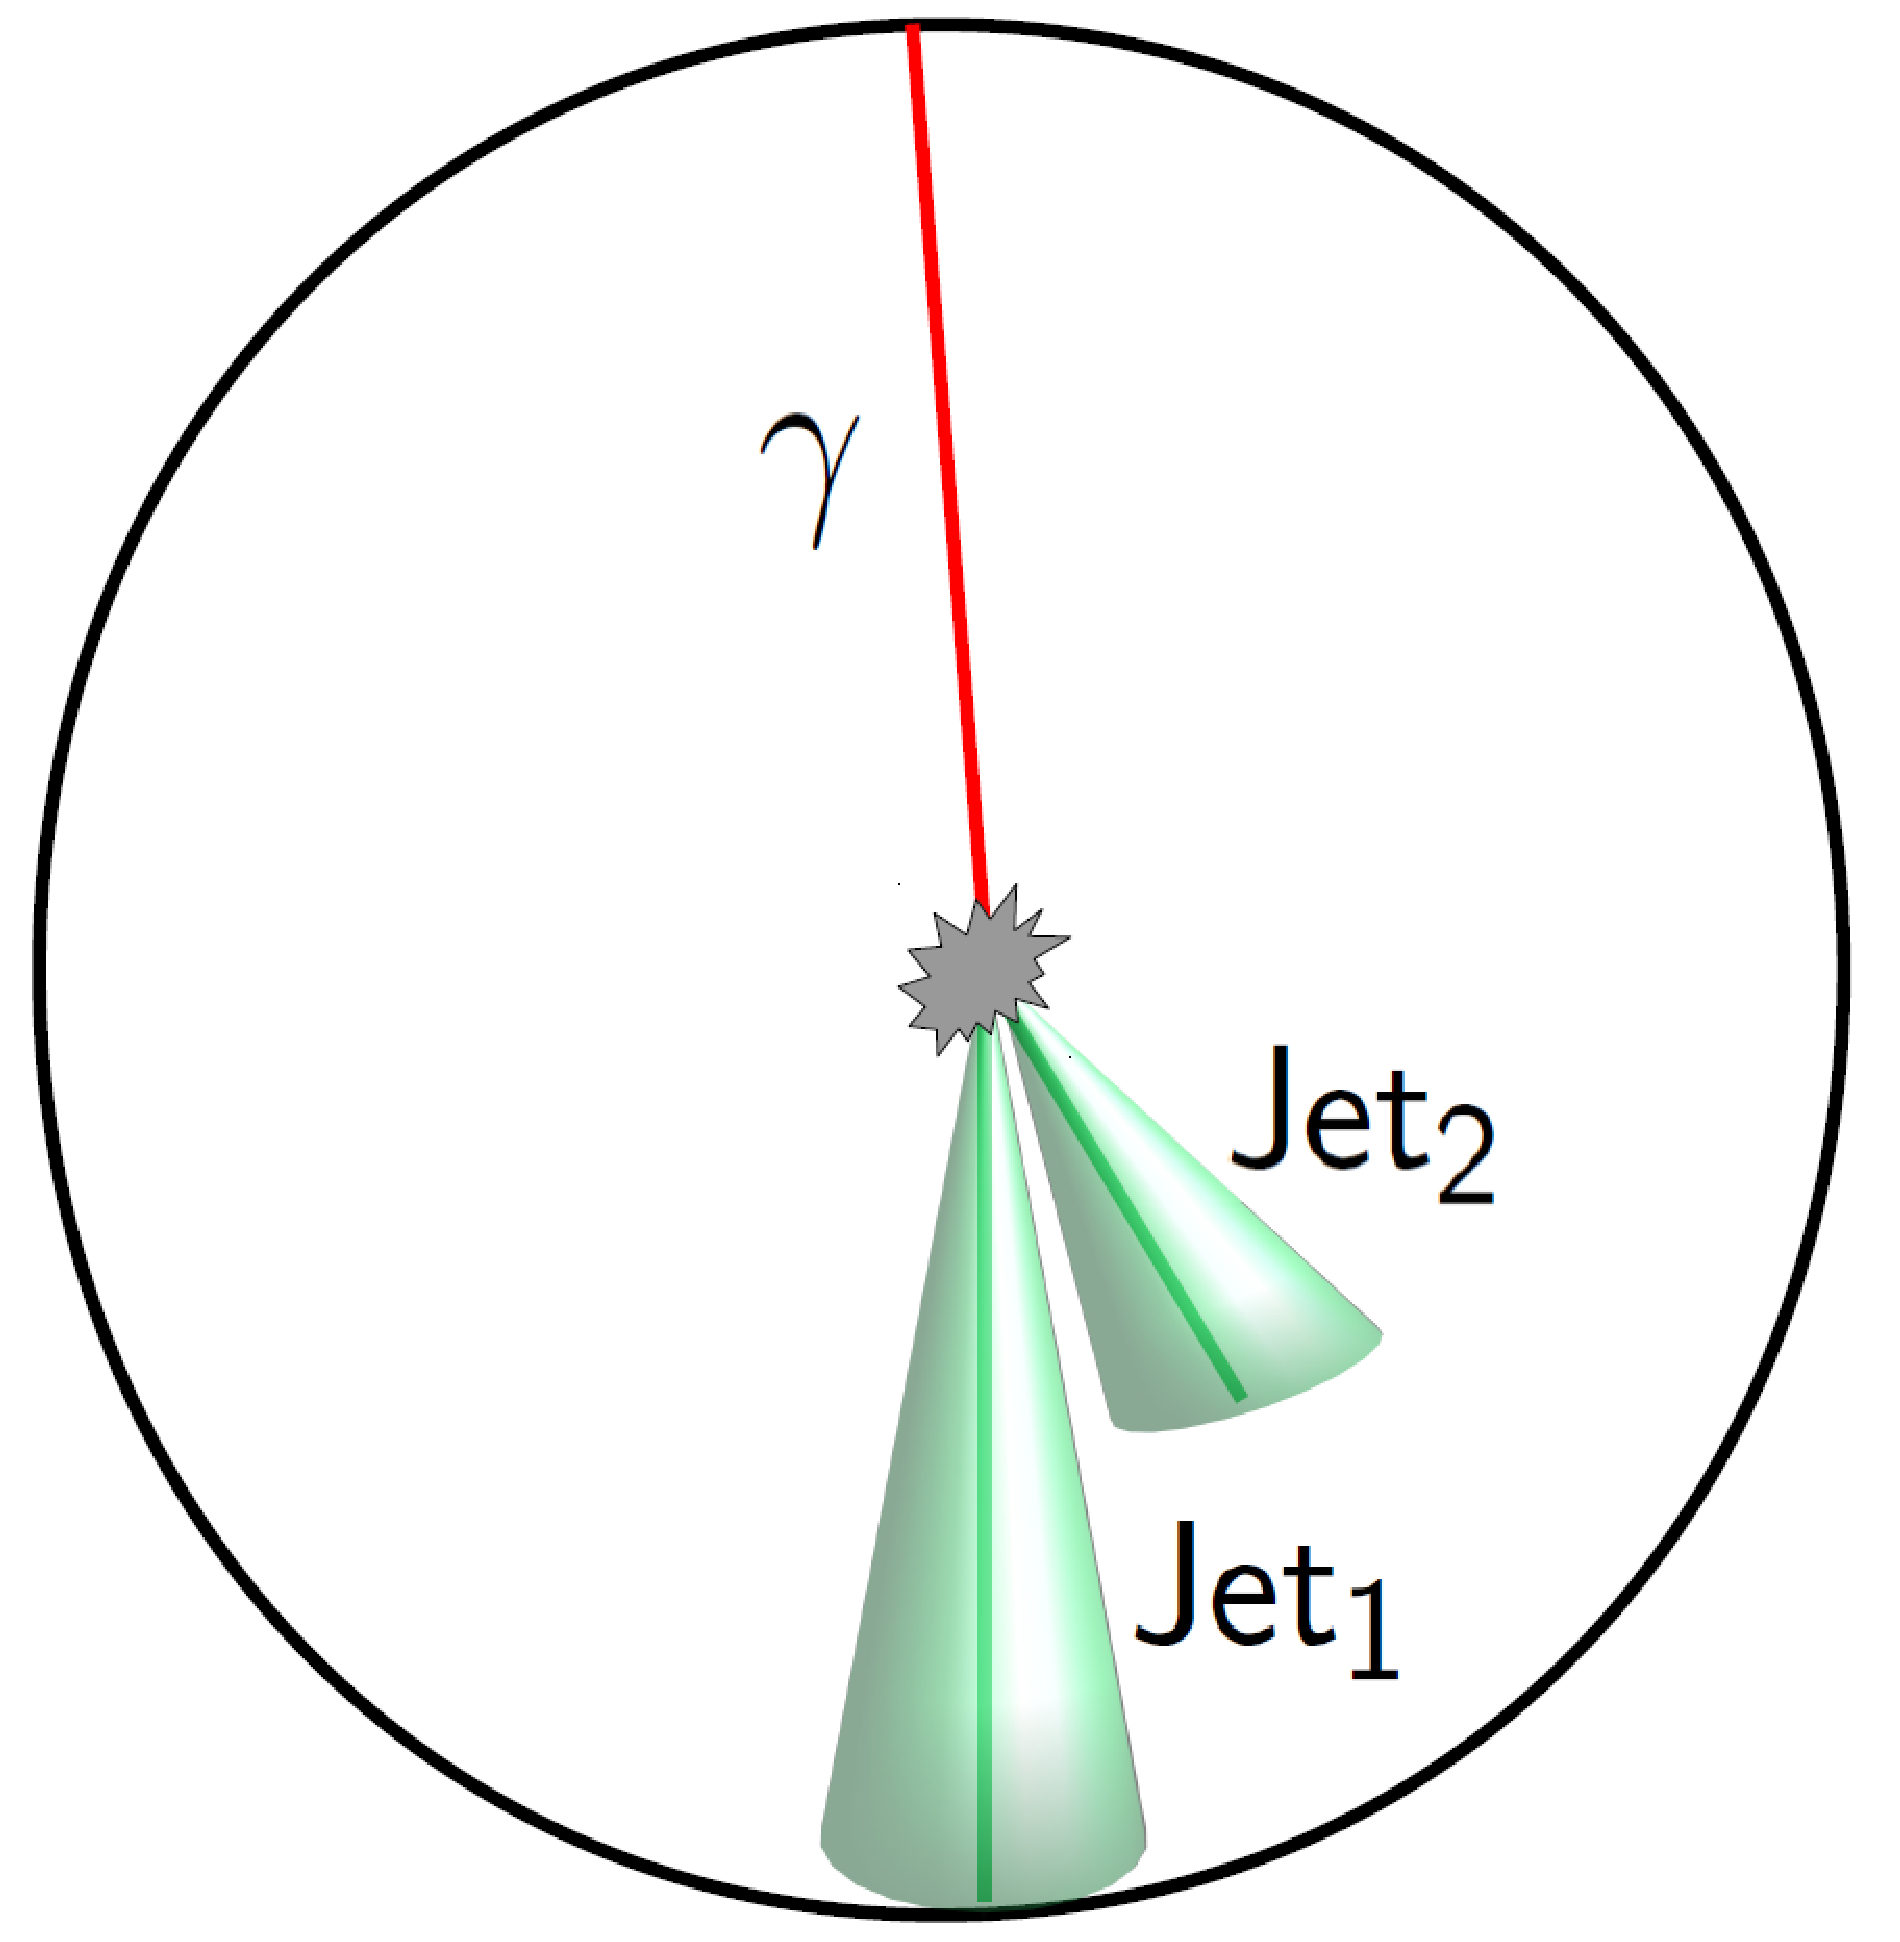
\includegraphics[width=0.42\textwidth]{figures/resolution/methodology/2ndJet_in_JetHemisphere.pdf}
     \hspace{0.1\textwidth}
     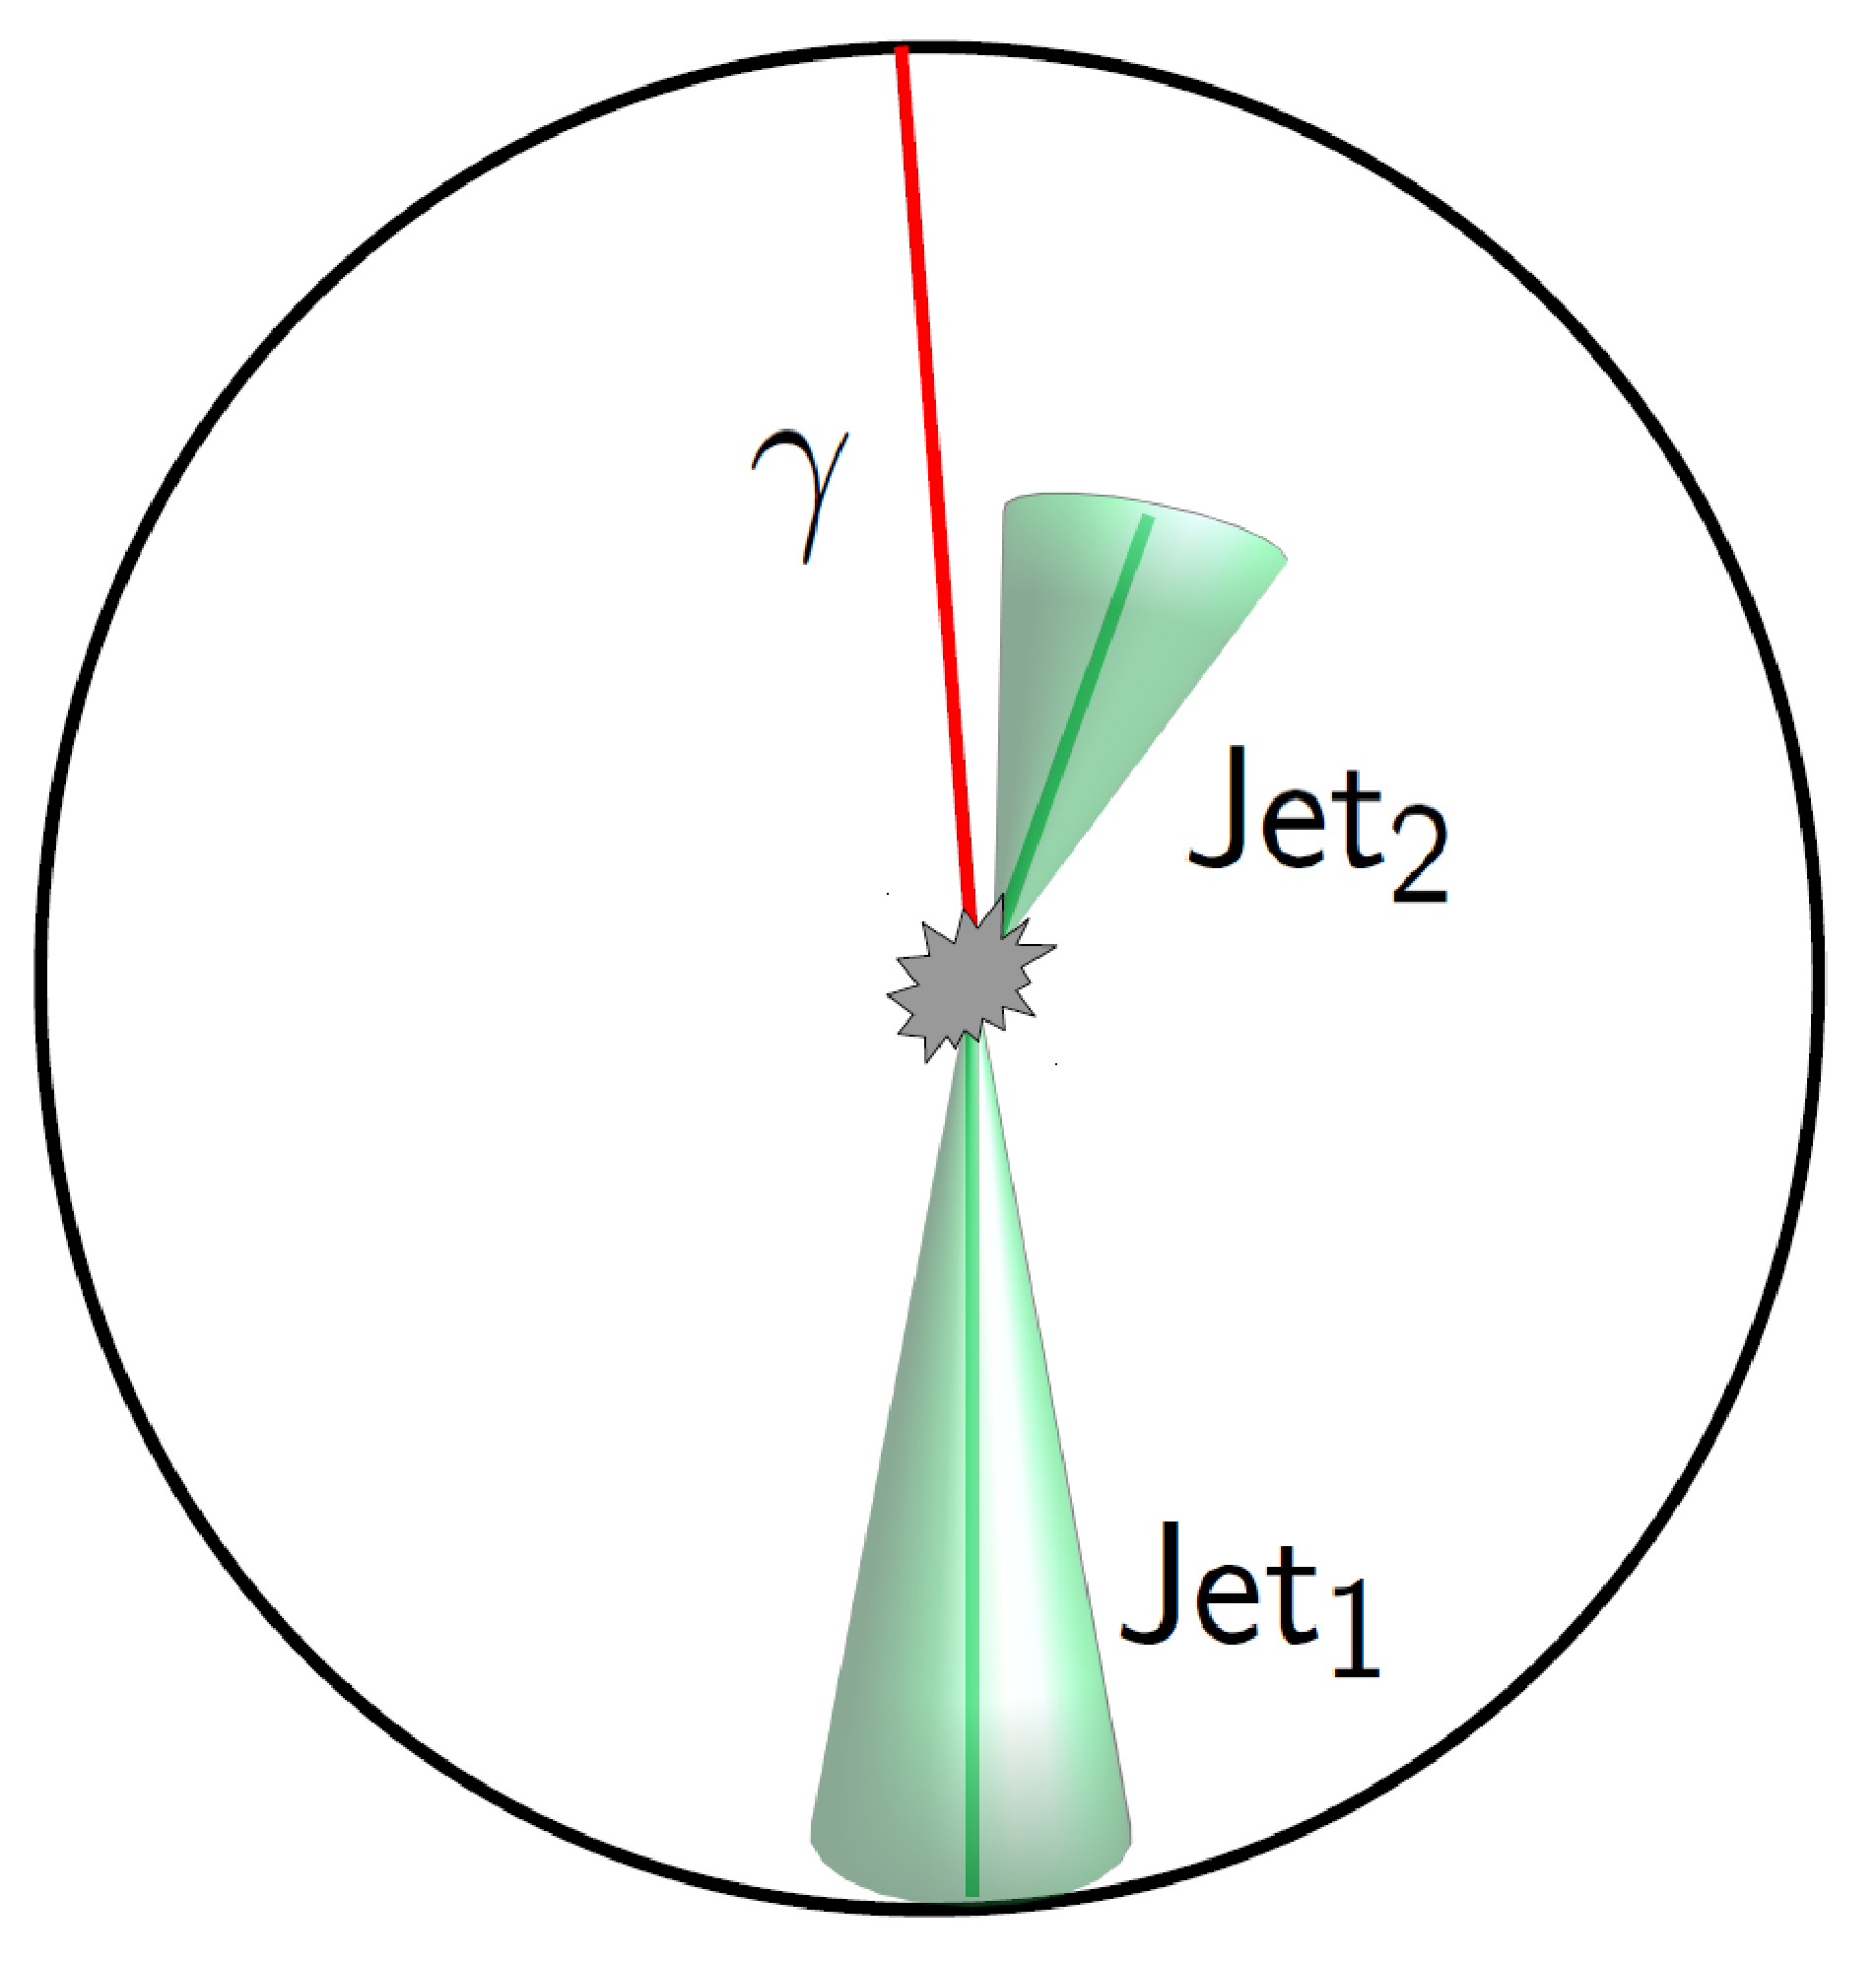
\includegraphics[width=0.42\textwidth]{figures/resolution/methodology/2ndJet_in_PhotonHemisphere.pdf}
  \caption{A schematic sketch of the two different event topologies where the second jet is in the leading jet (left) or the photon hemisphere (right)}  
 \label{fig:sketch}
\end{figure}

As can be seen in Fig.~\ref{fig:fullResponseAndContributions}, events containing a second jet in the leading jet hemisphere lead to a response histogram with mean smaller one, while events with a second jet in photon direction result in a distribution with mean larger one. 
The former occurs more frequently because it contains jets from final and initial state radiation, while the latter mainly consists only from initial state radiation.

The two response distributions coming from the different event topologies are separately evaluated. First, the resolution is determined for each of the configurations 
(cf. Fig.~\ref{fig:fullResponseAndContributions}), and then, the weighted mean of the two contributions is calculated.\\
\begin{figure}[!t]
  \centering
      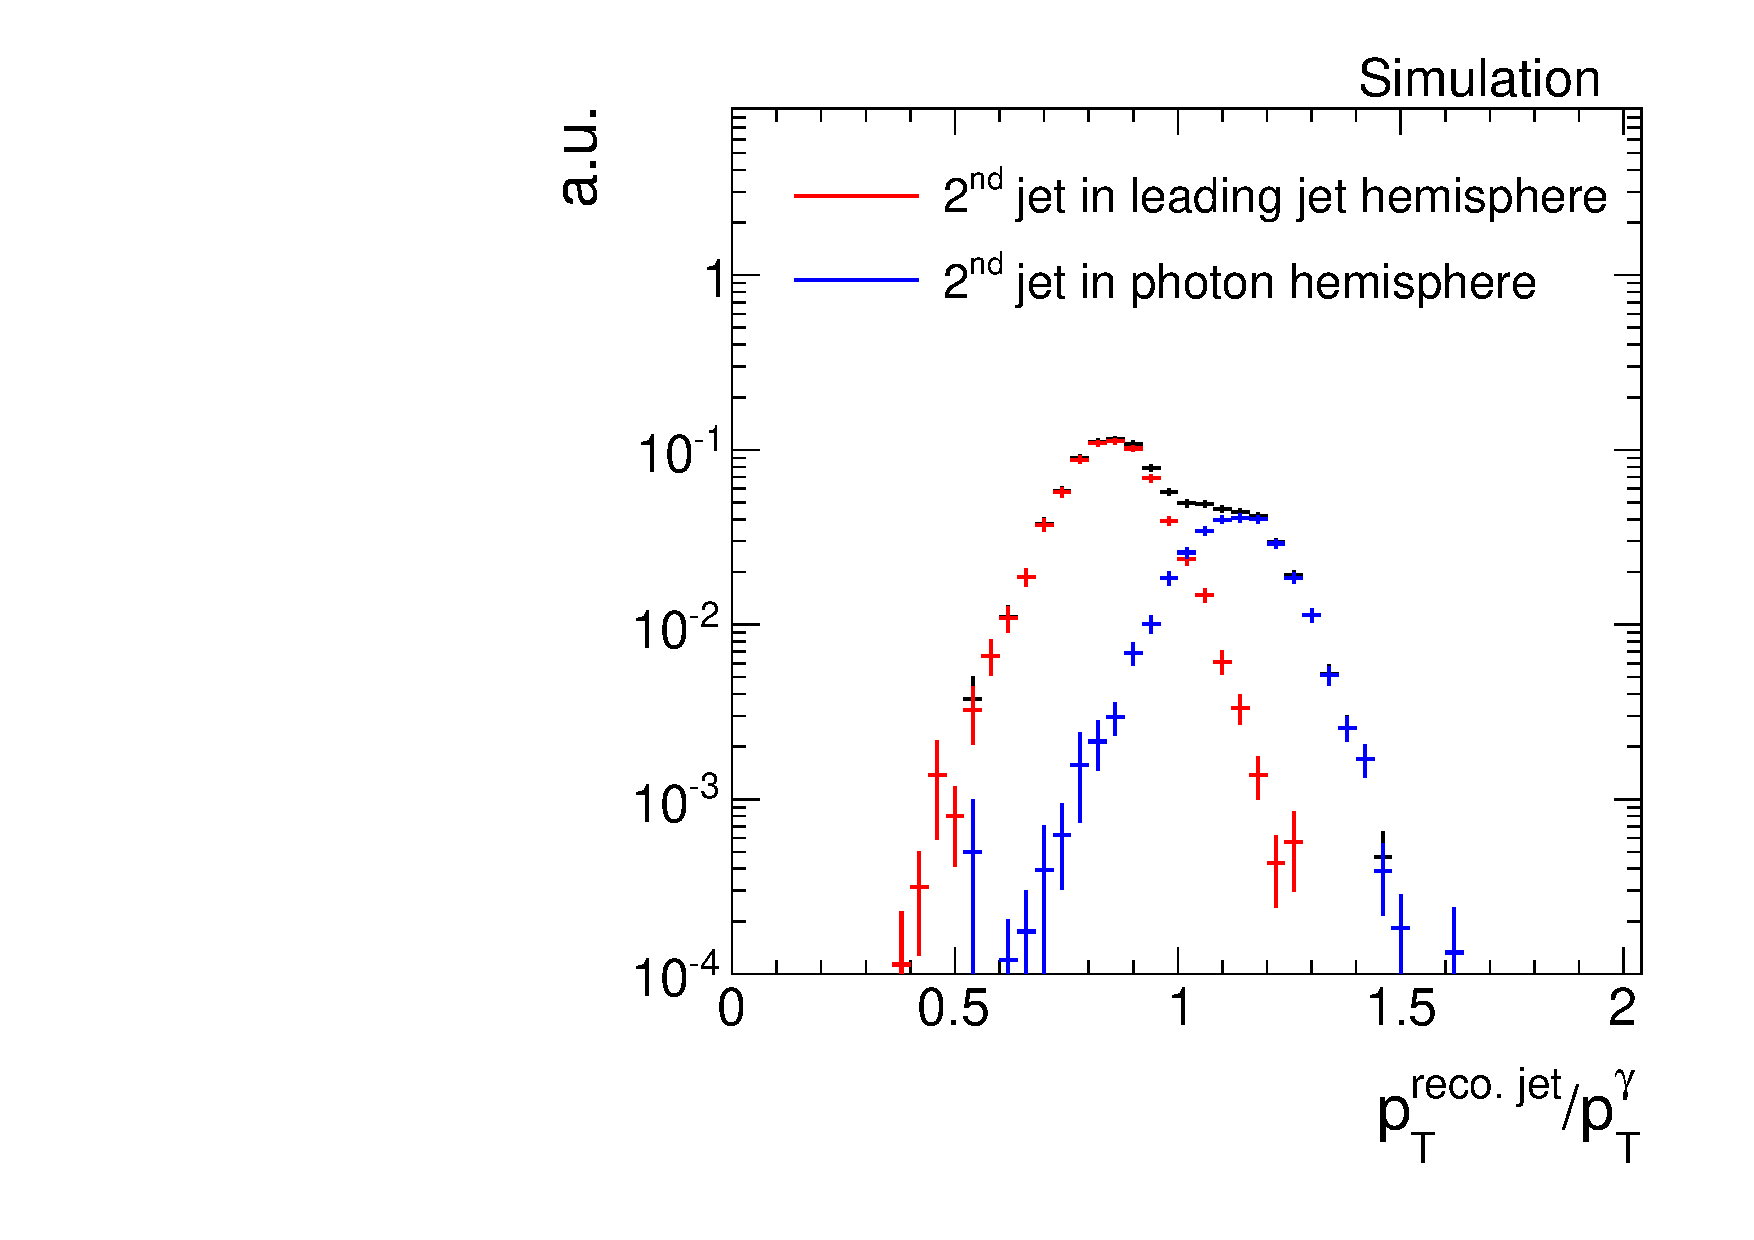
\includegraphics[width=0.49\textwidth]{figures/resolution/methodology/fullResponseAndContributions_6_alpha_bin.pdf}
  \caption{The measured response with the two contributions visualised. Events with a second jet in photon hemisphere (red) lead to a mean response larger one, while events with a
           second jet in the leading jet hemisphere (green) have a mean smaller one.}  
  \label{fig:fullResponseAndContributions}
\end{figure}

%These two different contributions (second jet in photon/leading jet hemisphere) result in two separate response distribution.
%A schematic sketch of the two contributions is shown in Fig.~\ref{fig:sketch}. 
%The double peak structure is less pronounced for small second jet \pt (small $\alpha$) where the $\Delta \Phi$ requirement does not have such a strong effect in rejecting
%events with a second jet perpendicular to the photon leading jet axis (see \mbox{Fig. \ref{fig:alphaBins}}).
%\begin{figure}[b]
% \centering
%     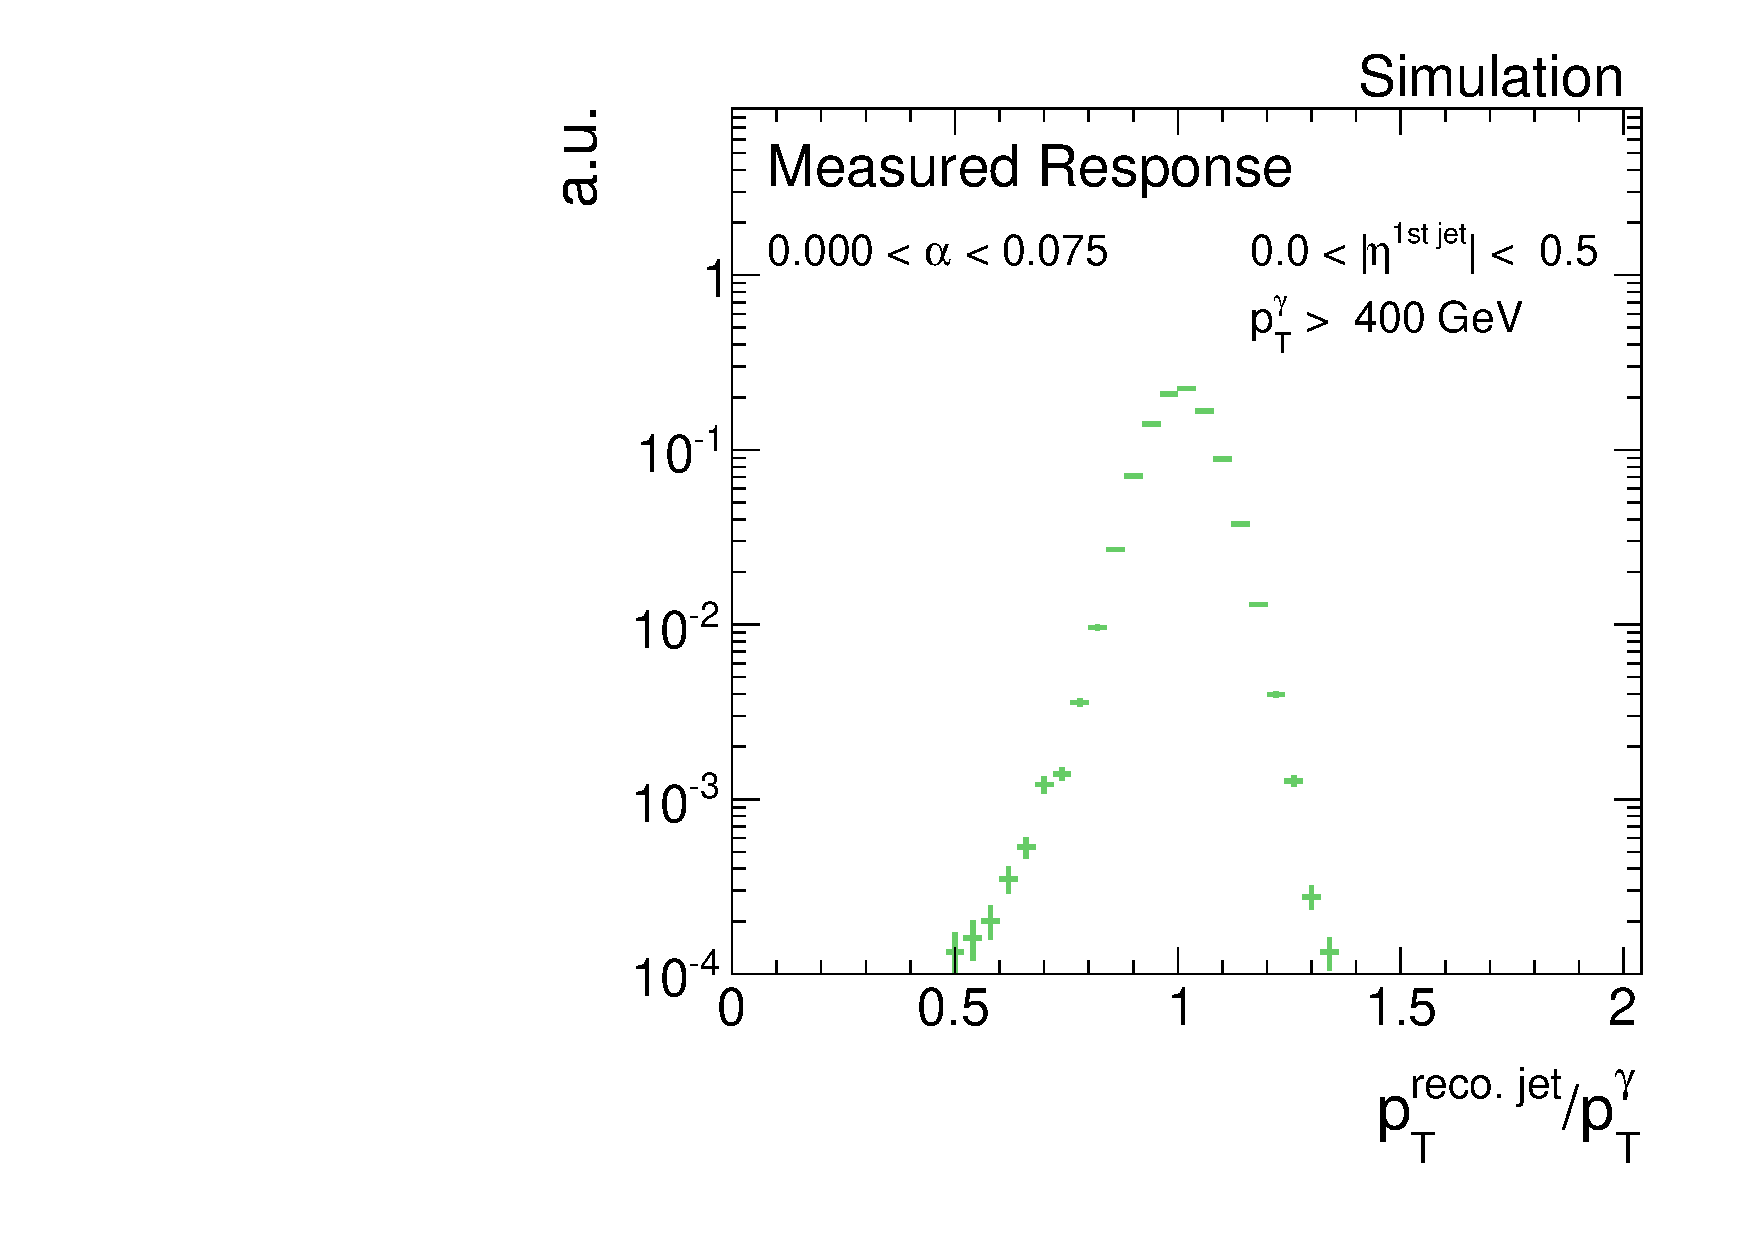
\includegraphics[width=0.32\textwidth]{figures/resolution/methodology/fullResponse_1_alpha_bin.pdf}
%     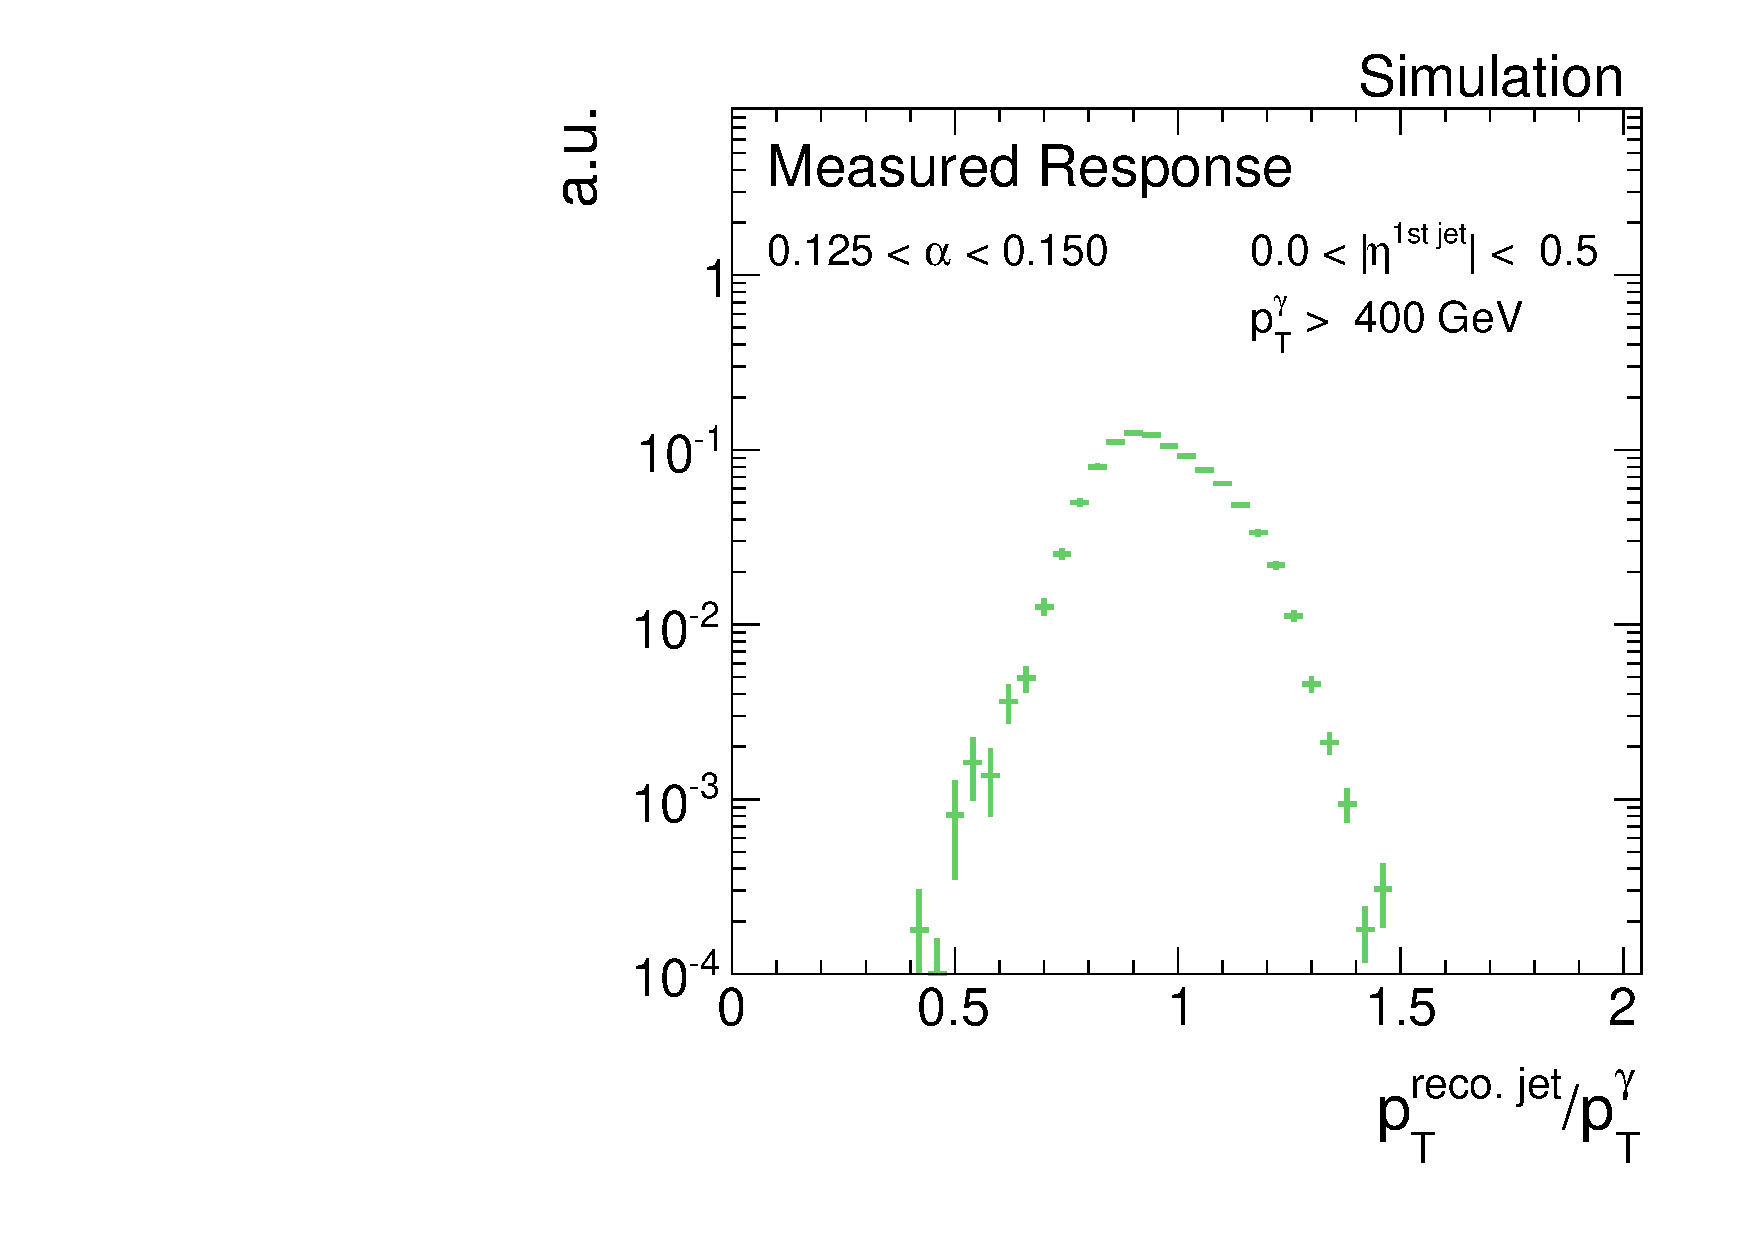
\includegraphics[width=0.32\textwidth]{figures/resolution/methodology/fullResponse_4_alpha_bin.pdf}
%     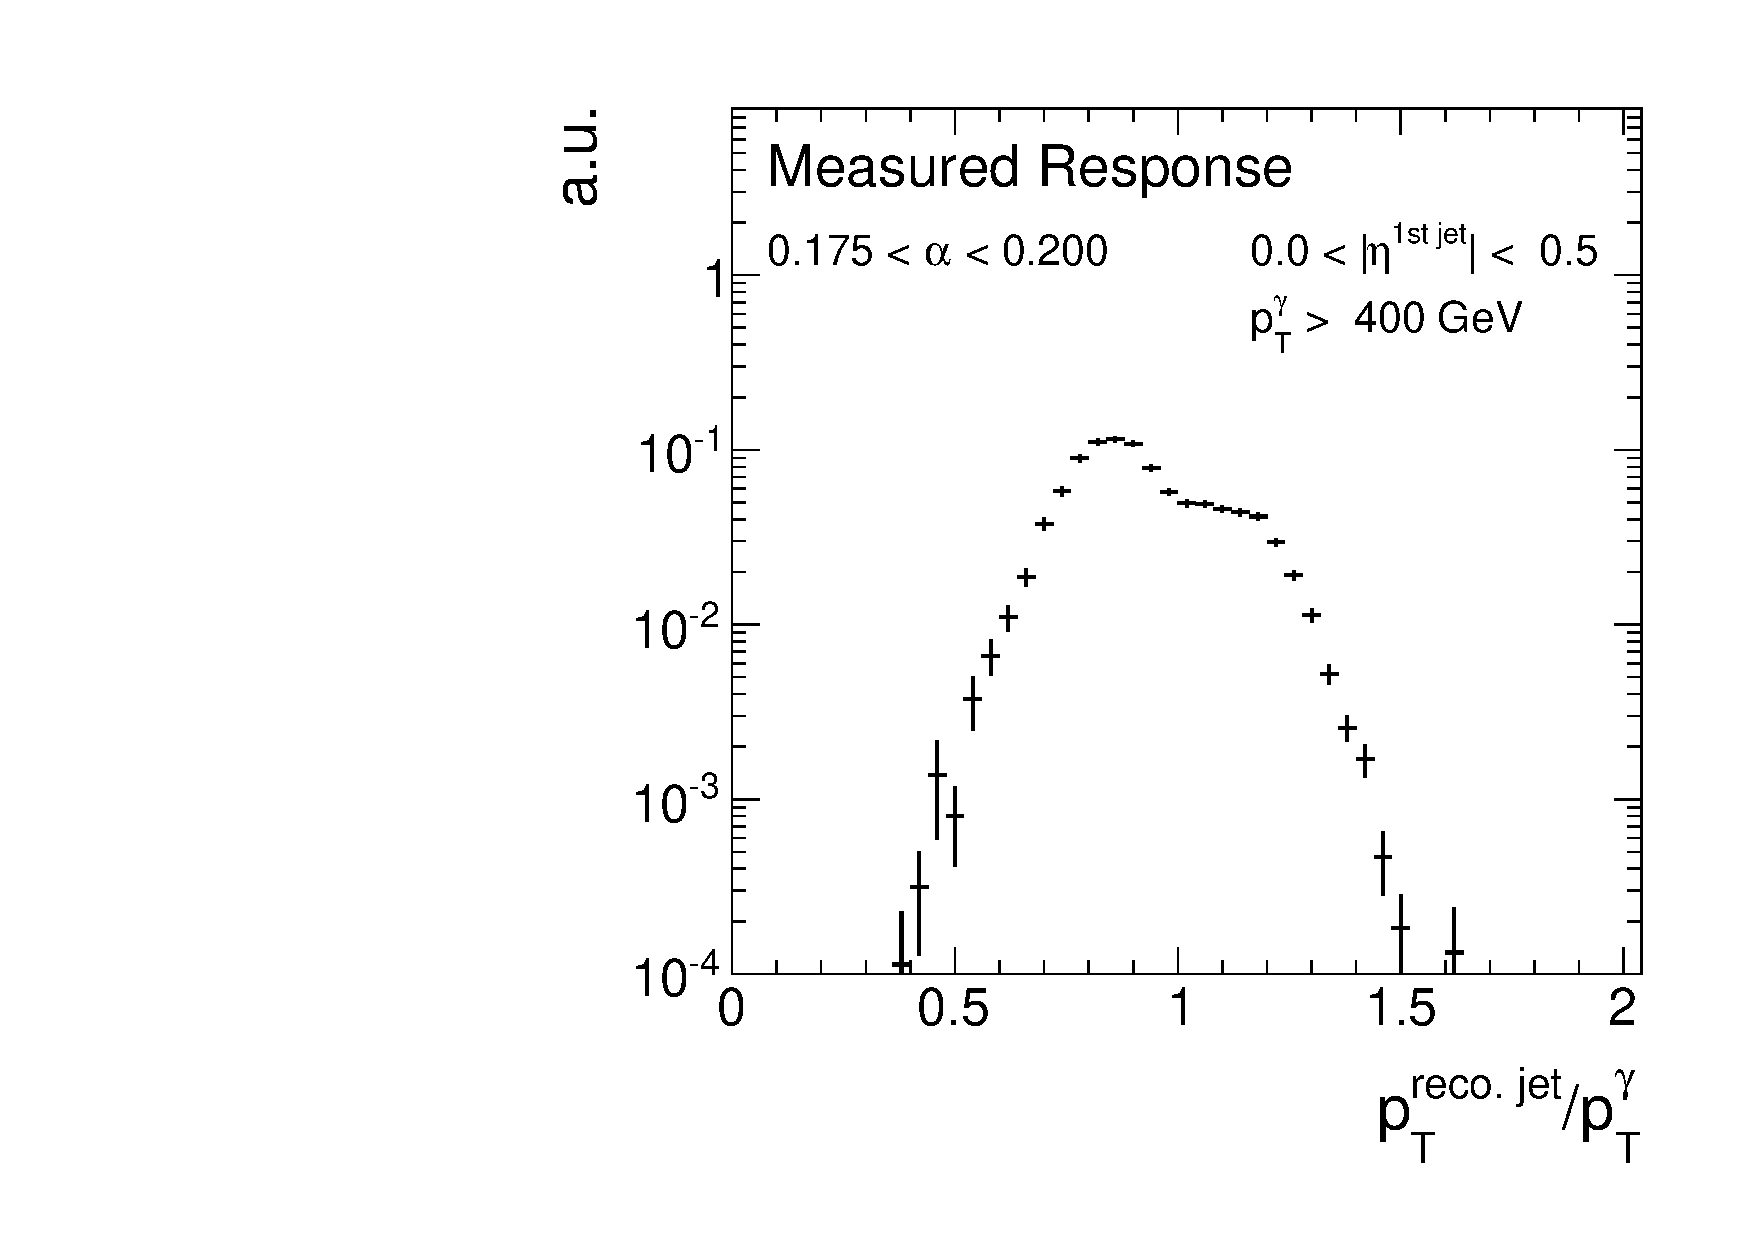
\includegraphics[width=0.32\textwidth]{figures/resolution/methodology/fullResponse_6_alpha_bin.pdf}
%  \caption{The measured response \ptrecojet/\ptgamma in simulation for FIXME : $\ptgamma < 400 \gev$ for three different $\alpha$ ranges: $0.0-7.5\%$ (left), $12.5-15.0\%$ (middle) and $17.5-20.0\%$ (right). 
%           It can be seen that the double peak structure gets less pronounced for low $\alpha$ values.}  
% \label{fig:alphaBins}
%\end{figure}


With the above presented methodology, it is possible to measure the resolution in simulation and data for different values of $\alpha$.
Since the quantity of interest is the jet transverse-momentum resolution independent of further jet activity, \ie the extrapolated value of the measured resolution at $\alpha=0$, 
the dependency of the measured resolution on alpha, $\jermeasured \left( \alpha \right)$, is needed.
Simulated data offers the possibility to study the individual contributions to the measured resolution, the intrinsic resolution $\jerintrinsic\left( \alpha \right)$ and the imbalance $\jerimbalance\left( \alpha \right)$.%, because generator-level information is available.

The intrinsic part of the resolution for a given photon \pt bin is, by definition, independent of secondary jet \pt, and can be considered as constant in terms of $\alpha$
\begin{equation}\label{eq:intrinsic}
 \jerintrinsic \left( \alpha\right) = c.
\end{equation}
This is not true for the imbalance part. 
It was found empirically that the $\alpha$ dependence of the imbalance can be described by a linear function~\cite{CMS:PAS:JETResolution_7TeV} 
\begin{equation}\label{eq:imbalance}
  \jerimbalance \left( \alpha\right) = q + m \cdot \alpha
\end{equation}
Folding two independent Gaussian functions results in a quadratic addition of the corresponding standard deviations $\jerintr\oplus\jerimb$ and finally yields the functional expression for the measured resolution
\begin{equation}\label{eq:total}
  \jermeasured \left( \alpha \right) = \sqrt{ c^2 + q^2  + 2\, q\, m \cdot \alpha +m^2 \cdot \alpha^2}. 
\end{equation}
In Fig.~\ref{fig:AlphaDependenceOfResolutions}, the $\alpha$ dependence of the intrinsic resolution (red dots), the imbalance (blue dots), and the measured resolution (green dots) is shown for two exemplary \ptgamma regions in simulated events. 
\begin{figure}[!b]
 \centering
    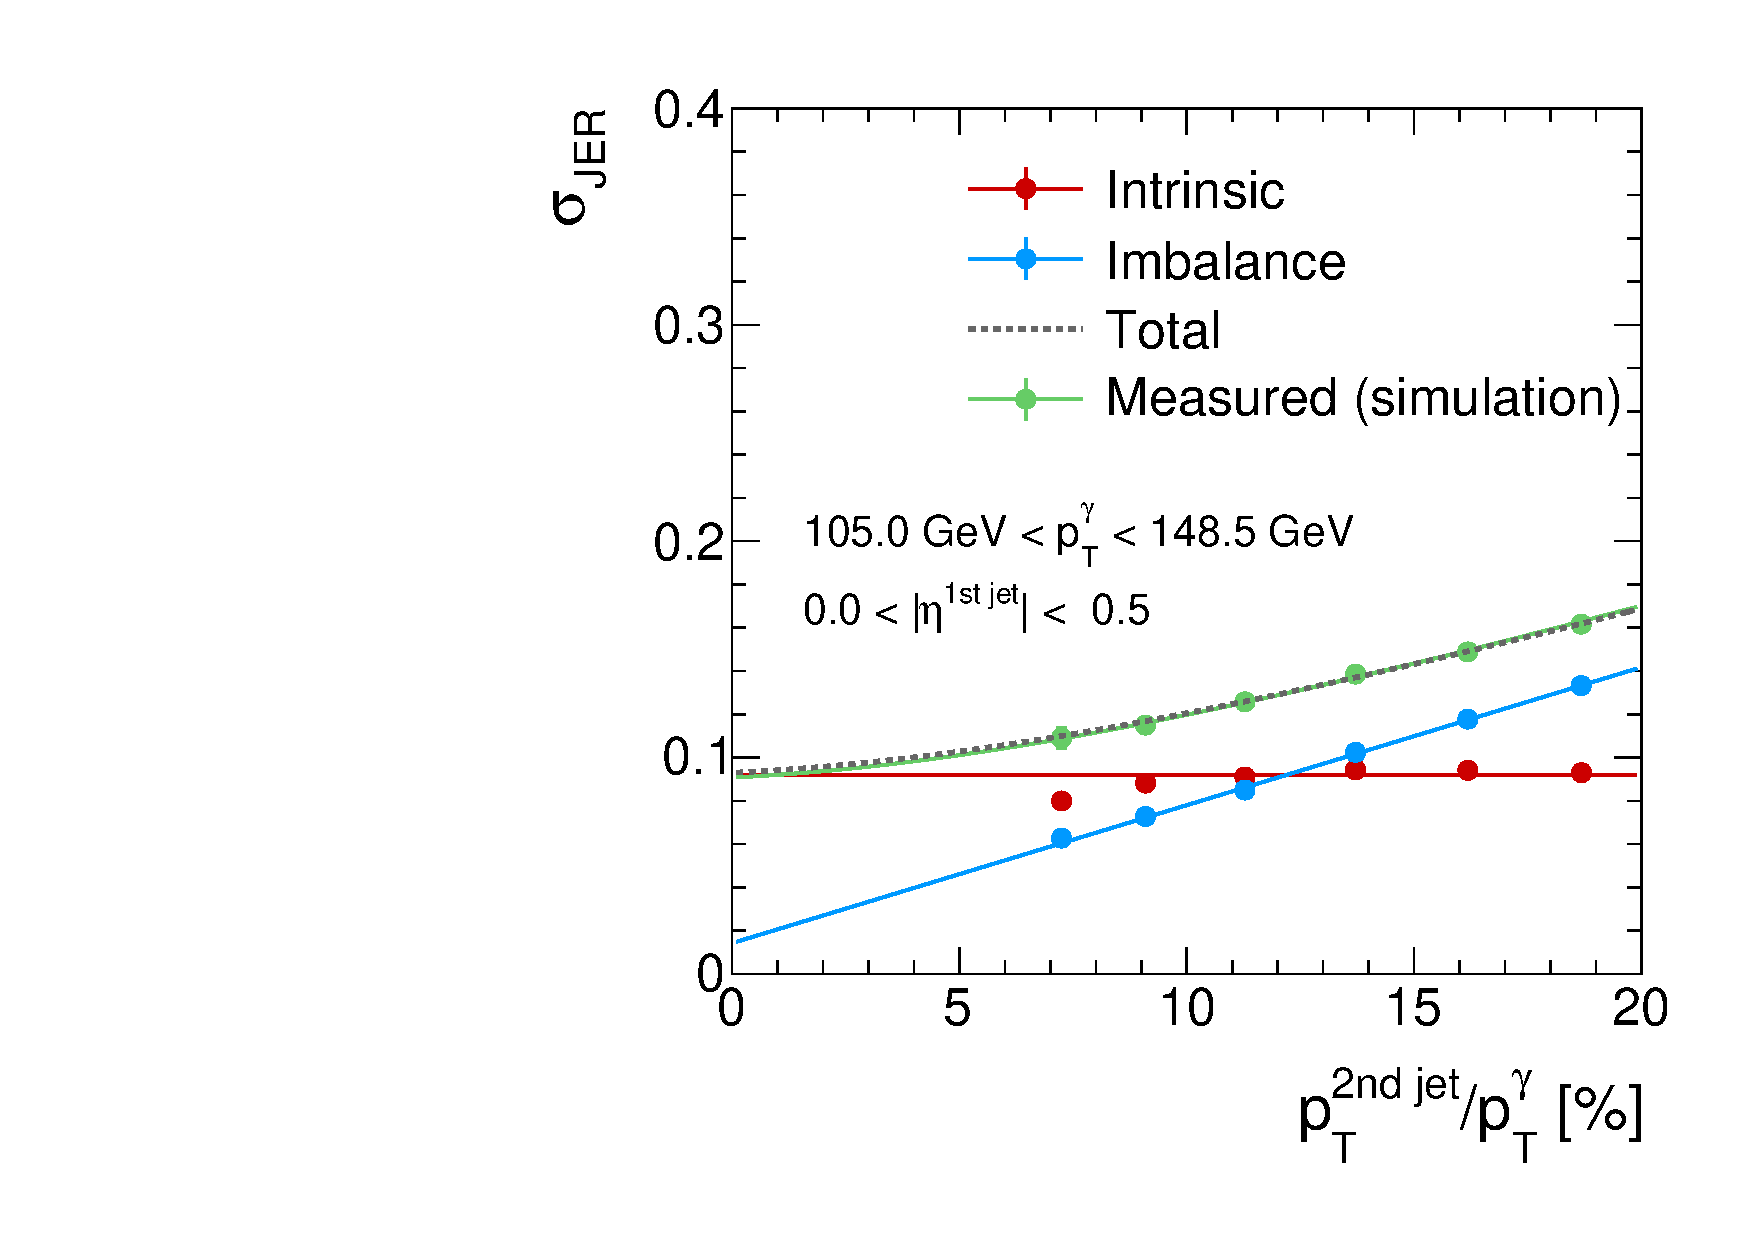
\includegraphics[width=0.49\textwidth]{figures/resolution/methodology/JER_for_1_eta_bin_5_pTGamma_bin_wo_data_PFCHS_RMS99_mc.pdf} 
    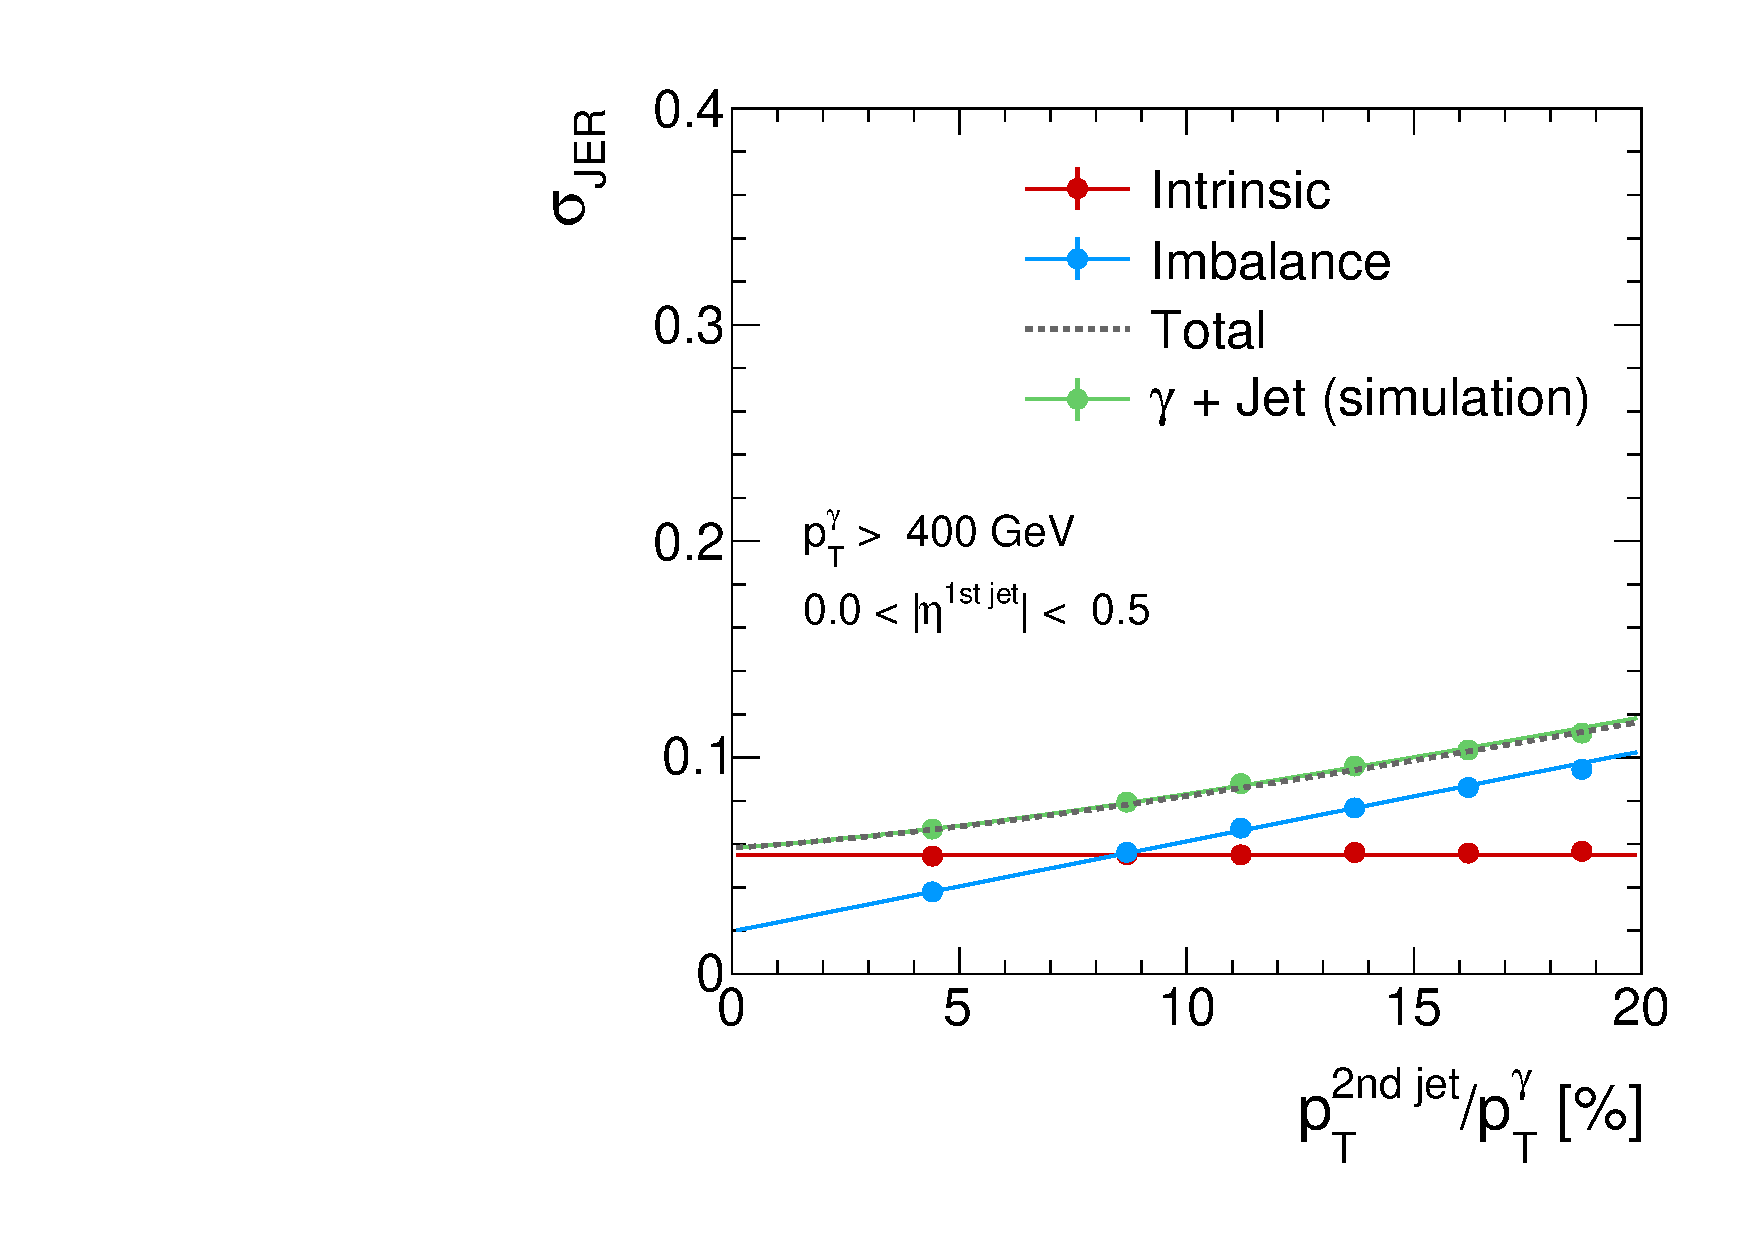
\includegraphics[width=0.49\textwidth]{figures/resolution/methodology/JER_for_1_eta_bin_12_pTGamma_bin_wo_data_PFCHS_RMS99_mc.pdf} 
  \caption{The alpha dependency of the various parts of the resolution in the simulated events for $83 \gev < \pt^{\gamma} < 99 \gev $ (left) and $400 \gev < \pt^{\gamma}$ (right). 
           The total resolution (grey dotted line) is the addition in quadrature of the imbalance (blue line) and the intrinsic (red line) fit functions. 
           It can be compared to the measured resolution in simulated data (green dots/line).}  
 \label{fig:AlphaDependenceOfResolutions}
\end{figure}
The intrinsic resolution is fitted with Eq.~\eqref{eq:intrinsic} (red line), while the imbalance is fitted with Eq.~\eqref{eq:imbalance} (blue line).

It is apparent that the imbalance is not zero for $\alpha=0$. 
This has two reasons.
First and most important, only the photon and the parton are balanced in the transverse plane.
But since the transverse momentum of a jet is defined as the sum of all particles' transverse momenta that are clustered into the jet cone, the jet \pt can be lower than the \pt of the original parton.
This effect is called out-of-cone showering and leads to a residual imbalance between the photon \pt and the generator-level jet \pt at $\alpha=0$ (parameter $q$ in Eq.~\eqref{eq:imbalance}).
Second, the photon \pt can be wrongly measured and spoil the residual imbalance $q$. 

Due to the existence of a residual imbalance $q$, it is not possible to simply use the measured resolution at $\alpha=0$ as an estimator of the intrinsic resolution $c$.
This is already obvious from Eq.~\eqref{eq:total} which evaluates to $\jermeasured  = \sqrt{c^2 + q^2}$ at $\alpha=0$.

For the determination of the intrinsic resolution in data, the method relies on the residual imbalance information from simulation.
Practically, when fitting the measured resolution (Eq.\eqref{eq:total}) in real data, the residual imbalance $q$ is fixed to the value obtained from the imbalance fit (Eq~\ref{eq:imbalance}) in simulation.
The intrinsic resolution in real data can then be obtained by extracting the fit parameter $c$.
In the following the estimator of the intrinsic resolution (fit parameter $c$ from the measured resolution) will be referred to as $\jer$.

For consistency, the same approach is used for simulated data.
The fitted function of the measured resolution (green line) in Fig.~\ref{fig:AlphaDependenceOfResolutions} corresponds to the fit function of Eq.~\eqref{eq:total} with the parameter $q$ fixed to the value obtained from the imbalance fit (blue line).
Finally, the dotted grey line is the total resolution with the analytic expression of function \eqref{eq:total} with the parameters set to the fit values of the intrinsic (red) and the imbalance fit (blue). 
It can be nicely seen that the total resolution and the fit function of the measured resolution (green line) are well in agreement.
This implies, that the assumed functional forms of the resolution components and the assumed convolution leads indeed to a good description of the measured resolution.
Further validations of the methodology will be described in Section~\ref{res:sec:validation}.

%Figure~\ref{fig:ImbalanceOfPtgamma} shows the residual imbalance for two exemplary $|\etafirstjet|$ bins. 
%It is almost stable and around 2\% over the whole photon \pt range.
%\begin{figure}[b]
%  \centering
%    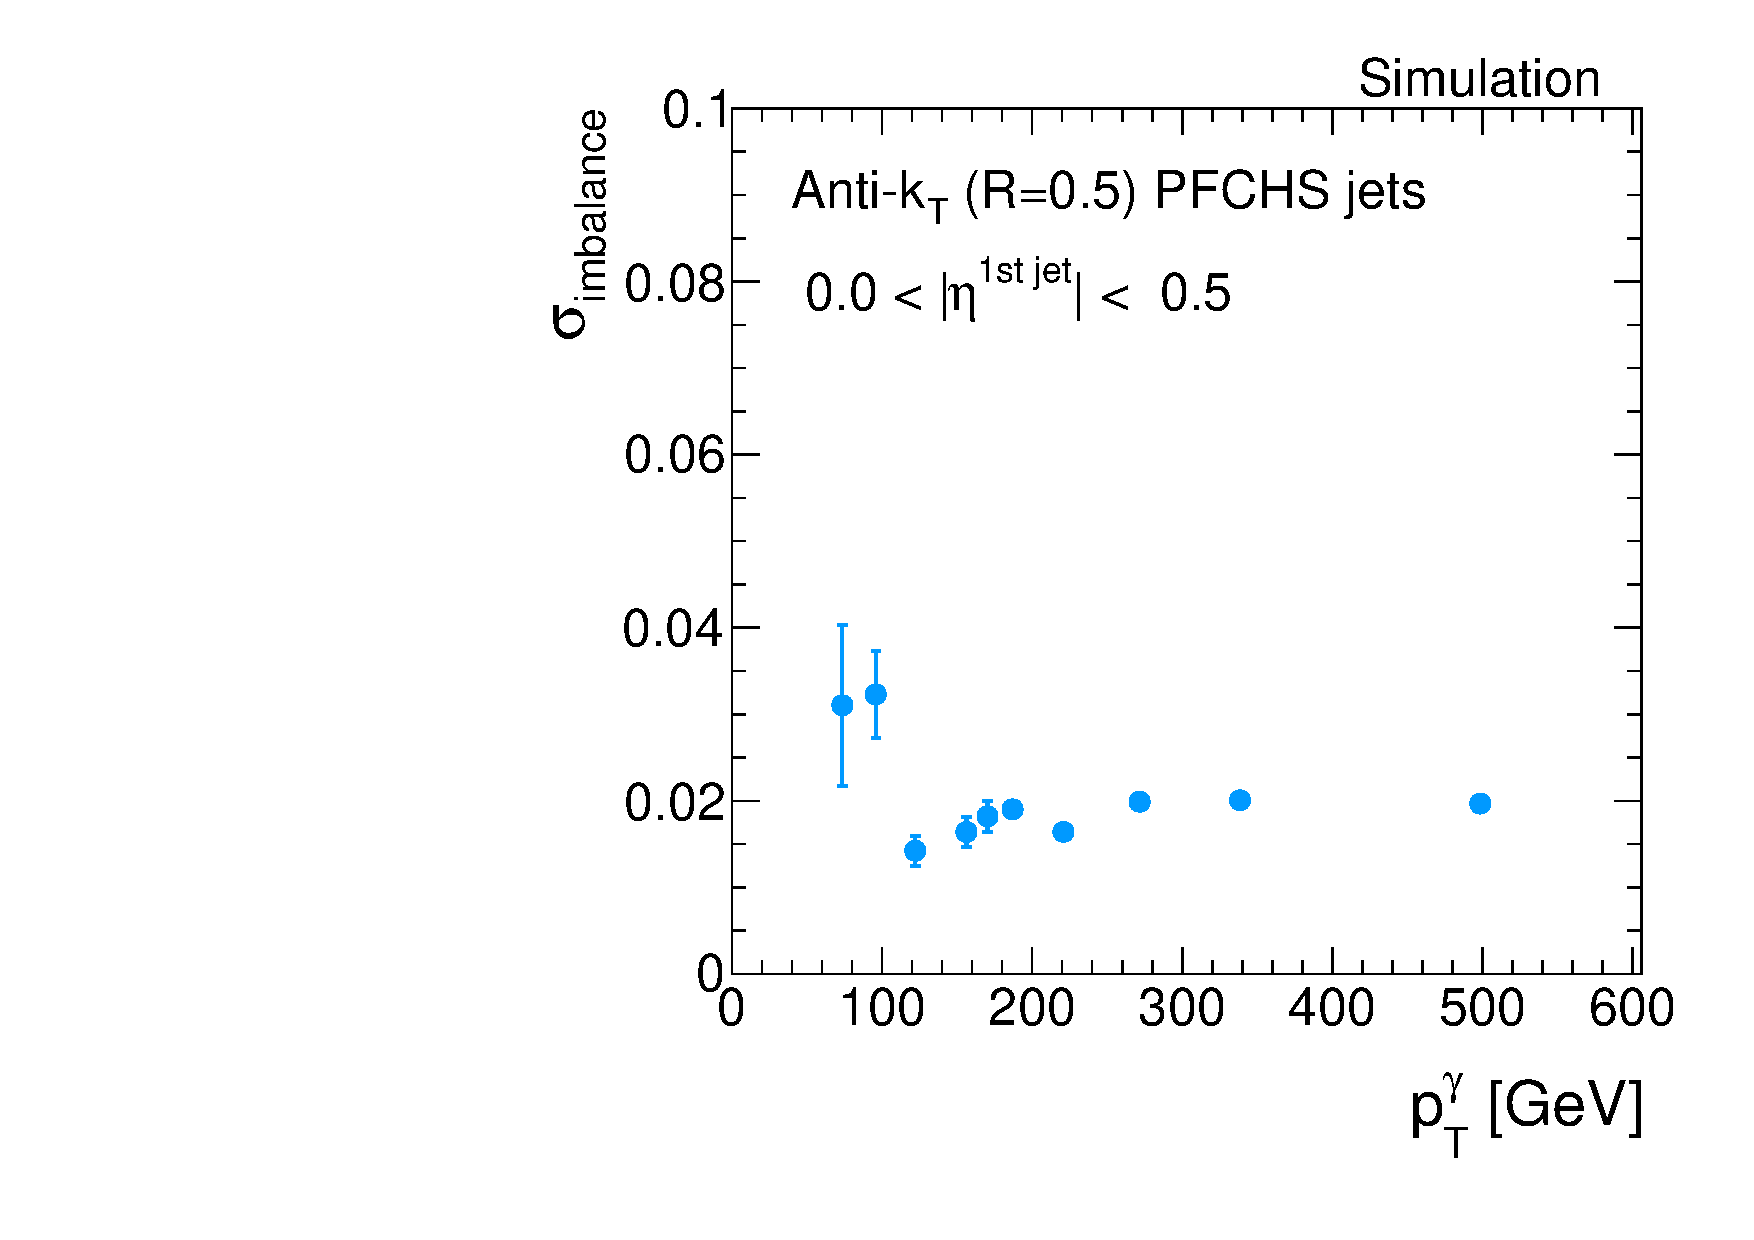
\includegraphics[width=0.49\textwidth]{figures/resolution/methodology/Imbalance_for_1_eta_bin_PFCHS_mc_RMS99.pdf}
%    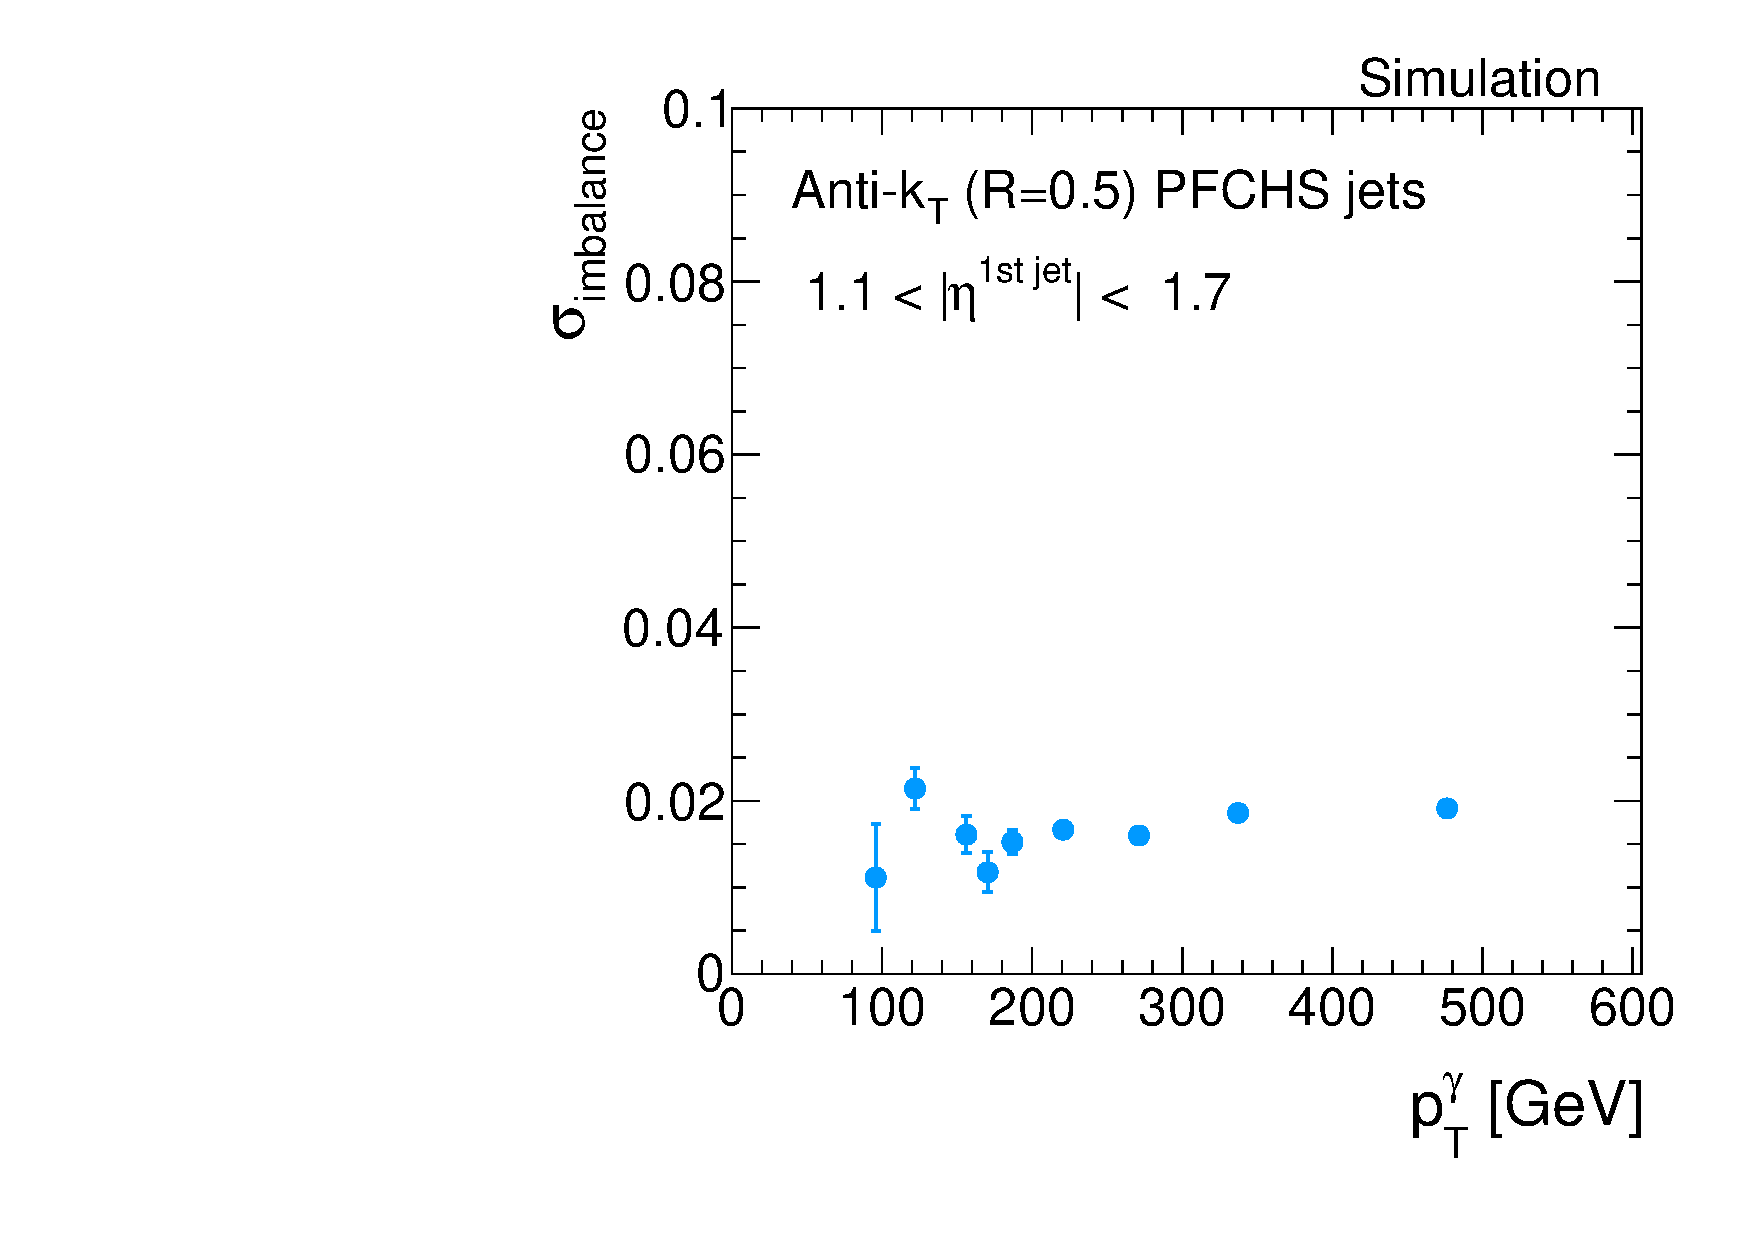
\includegraphics[width=0.49\textwidth]{figures/resolution/methodology/Imbalance_for_3_eta_bin_PFCHS_mc_RMS99.pdf}
%  \caption{Imbalance for $|\etafirstjet| < 0.5$ (left) and $1.1<|\etafirstjet| < 1.7$ (right) in simulation.}  
%  \label{fig:ImbalanceOfPtgamma}
%\end{figure}

In Fig.~\ref{fig:ResolutionOfPtgamma}, the extracted intrinsic resolution in simulation (green) and real data (black) is shown in different photon \pt bins for two different $|\etafirstjet|$ regions.
The resolution improves for increasing photon \pt. 
\begin{figure}[!b]
  \centering
    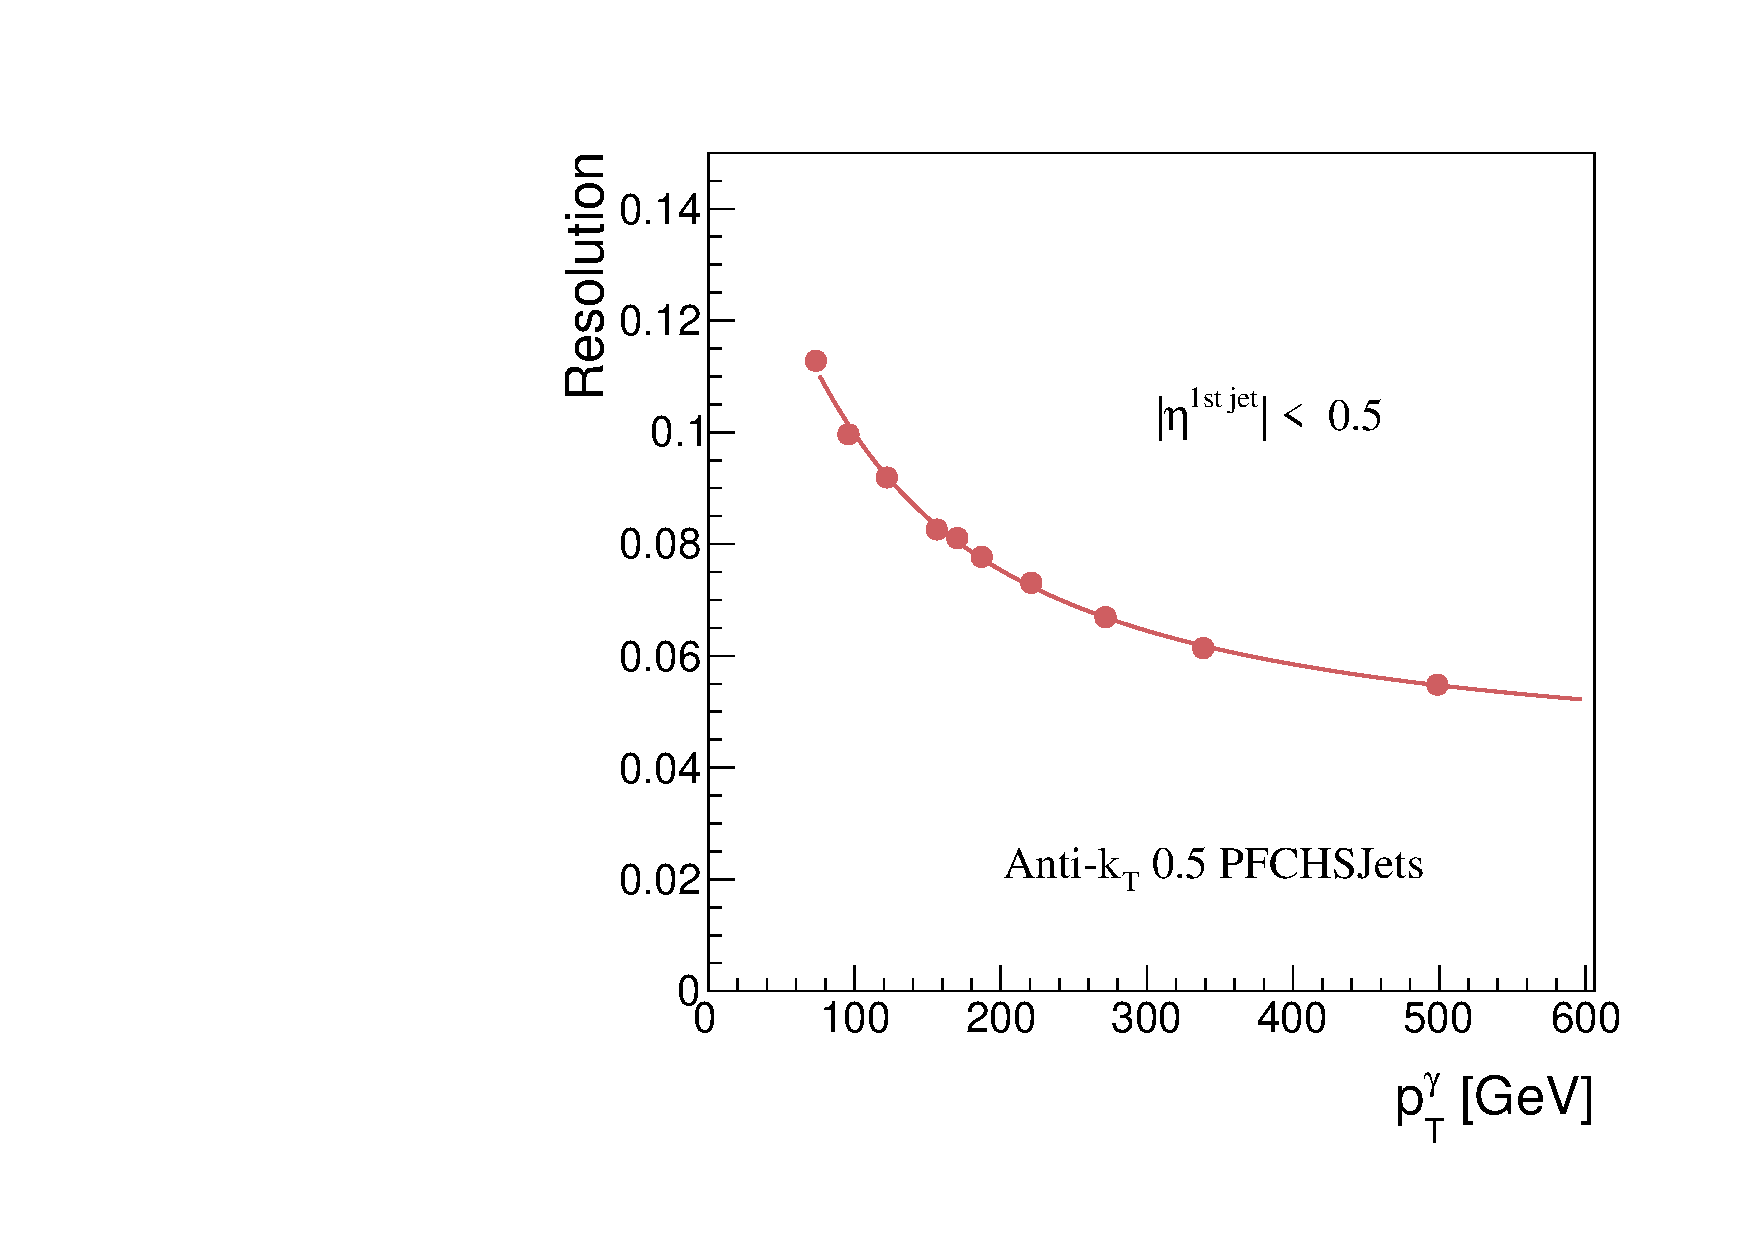
\includegraphics[width=0.49\textwidth]{figures/resolution/methodology/Resolution_for_1_eta_bin_PFCHS_mc_RMS99.pdf}
    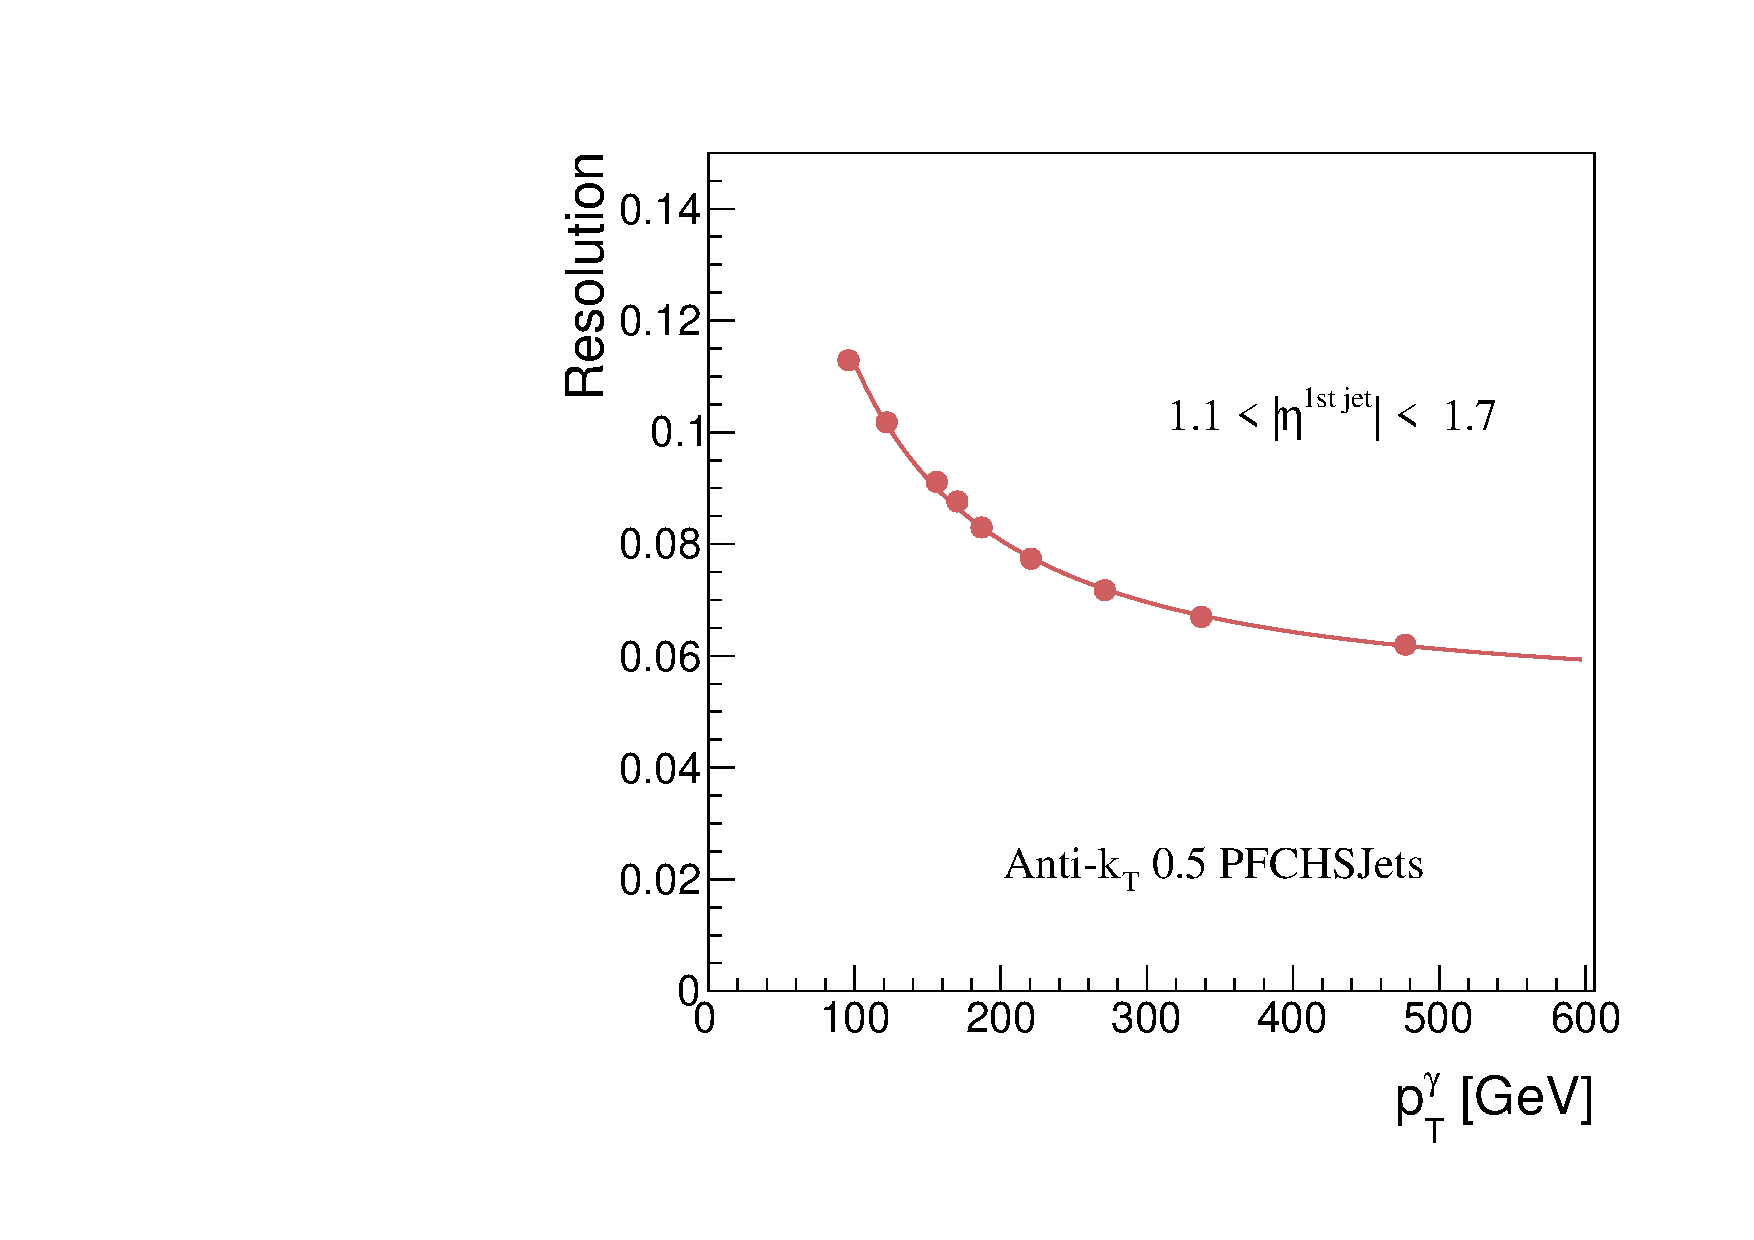
\includegraphics[width=0.49\textwidth]{figures/resolution/methodology/Resolution_for_3_eta_bin_PFCHS_mc_RMS99.pdf}
  \caption{Resolution for $|\etafirstjet| < 0.5$ (left) and $1.1<|\etafirstjet| < 1.7$ (right) in simulation (green) and real data (black). Both are fitted with a particle-flow resolution function introduced in~\cite{bib:CMS:JERCPaper_2011}.}  
  \label{fig:ResolutionOfPtgamma}
\end{figure}
For the $|\etafirstjet|<0.5$ region, the resolution is approximately 10\% for $\pt^{\gamma} \approx 100\gev$ and decreases to values around 6\% for  
$\pt^{\gamma} \approx 500\gev$.
The increasing statistical uncertainties for low photon \pt arise through the requirement of a maximal $\alpha$ and a minimal \pt of the second jet. 
This reduces the numbers of events in the low photon \pt bins. 
For events with $\ptgamma \lesssim 50\gev$, it is not possible at all to fulfil both requirements at the same time.

%The extrapolated intrinsic resolutions for the various photon \pt are fitted with the following function
%\begin{equation}
%\label{eq:PFresolution}
%\jer = \sqrt{\text{sgn(N)} \cdot \frac{\text{N}}{\pt}  + \text{S}^2 \cdot \pt^{\text{M}-1} +  \text{C}^2 }
%\end{equation}
%which was introduced for particle flow jets in~\cite{bib:CMS:JERCPaper_2011}.
%It is an extended fit function compared to the usual calorimeter resolution parametrisation to account for the higher resolution due to tracking information. 

From Fig.~\ref{fig:ResolutionOfPtgamma}, it can be seen that the resolution in data is always worse than the resolution in simulation.
Thus, in order to measure data-to-simulation scale factors \rhores for the jet transverse-momentum resolution, the measured resolution in data is divided by the resolution in Monte Carlo simulation (MC).
\begin{equation}
\label{res:eq:rhores}
\rhores = \frac{\jer^{\text{data}}}{\jer^{\text{MC}}}
\end{equation}
The results will show (Chapter~\ref{res:ch:results}), that this ratio is independent of \ptgamma and can thus be fitted with a constant in terms of \ptgamma.
The measurement of the data-to-simulation scale factors is therefore only done in bins of $|\etafirstjet|$.

How to apply these scale factors and adjust the jet transverse-momentum resolution in simulation to the measured resolution in data is well described in~\cite{bib:Matthias_Thesis}.


%Finally, in order to measure data-to-simulation scale factors \rhores for the jet transverse-momentum resolution, the measured resolution in data is divided by the resolution in Monte Carlo simulation (MC)
%\begin{equation}
%\label{res:eq:rhores}
%\rhores = \frac{\jer^{\text{data}}}{\jer^{\text{MC}}}
%\end{equation}
%It was found empirically, that this ratio is independent of \ptgamma, and can be fitted with a constant.
%Thus, to account for differences in the data-to-simulation ratio for different pseudorapidity ranges of the jet, the measurement of the scale factors is only done in bins of $|\etafirstjet|$.

%How to adjust finally the jet transverse-momentum resolution in simulation to the measured resolution in data is well described in~\cite{bib:Matthias_Thesis}.


%%%%%%%%%%%%%%%%%%%%%%%%%%%%%%%%%%%%%%%%%%%%%%%%%%%%%%%%%%%%%%%%%%%%%%%%%%%%%%%%%%%%%%%%%%%%%%%%%%%%%%%%%%%%%%%%%%%%%%%%%%%%%%%%%%%%%%%%%%%%%%%%%%%%%%%%%%%%%%%%%%%%%%%%%%%%%%%%%%%%%%%%%%%%%%%%%%%%%%%%%%%%%%%%%%%%%%%%%%%%%%%%%%%
\FloatBarrier
\section{Validation of the method}
\label{res:sec:validation}
It has already been shown that the decomposition of the measured resolution into intrinsic resolution and imbalance works well for the two shown \ptgamma bins in Fig.~\ref{fig:AlphaDependenceOfResolutions}.
In order to further validate the method, a comparison between \jer extracted from the measured resolution and the real \jer of the intrinsic resolution is performed on simulated events. 
Figure~\ref{fig:MCClosure} depicts the results of this comparison for one exemplary $|\etafirstjet|$ bin.
\begin{figure}[!b]
  \centering
    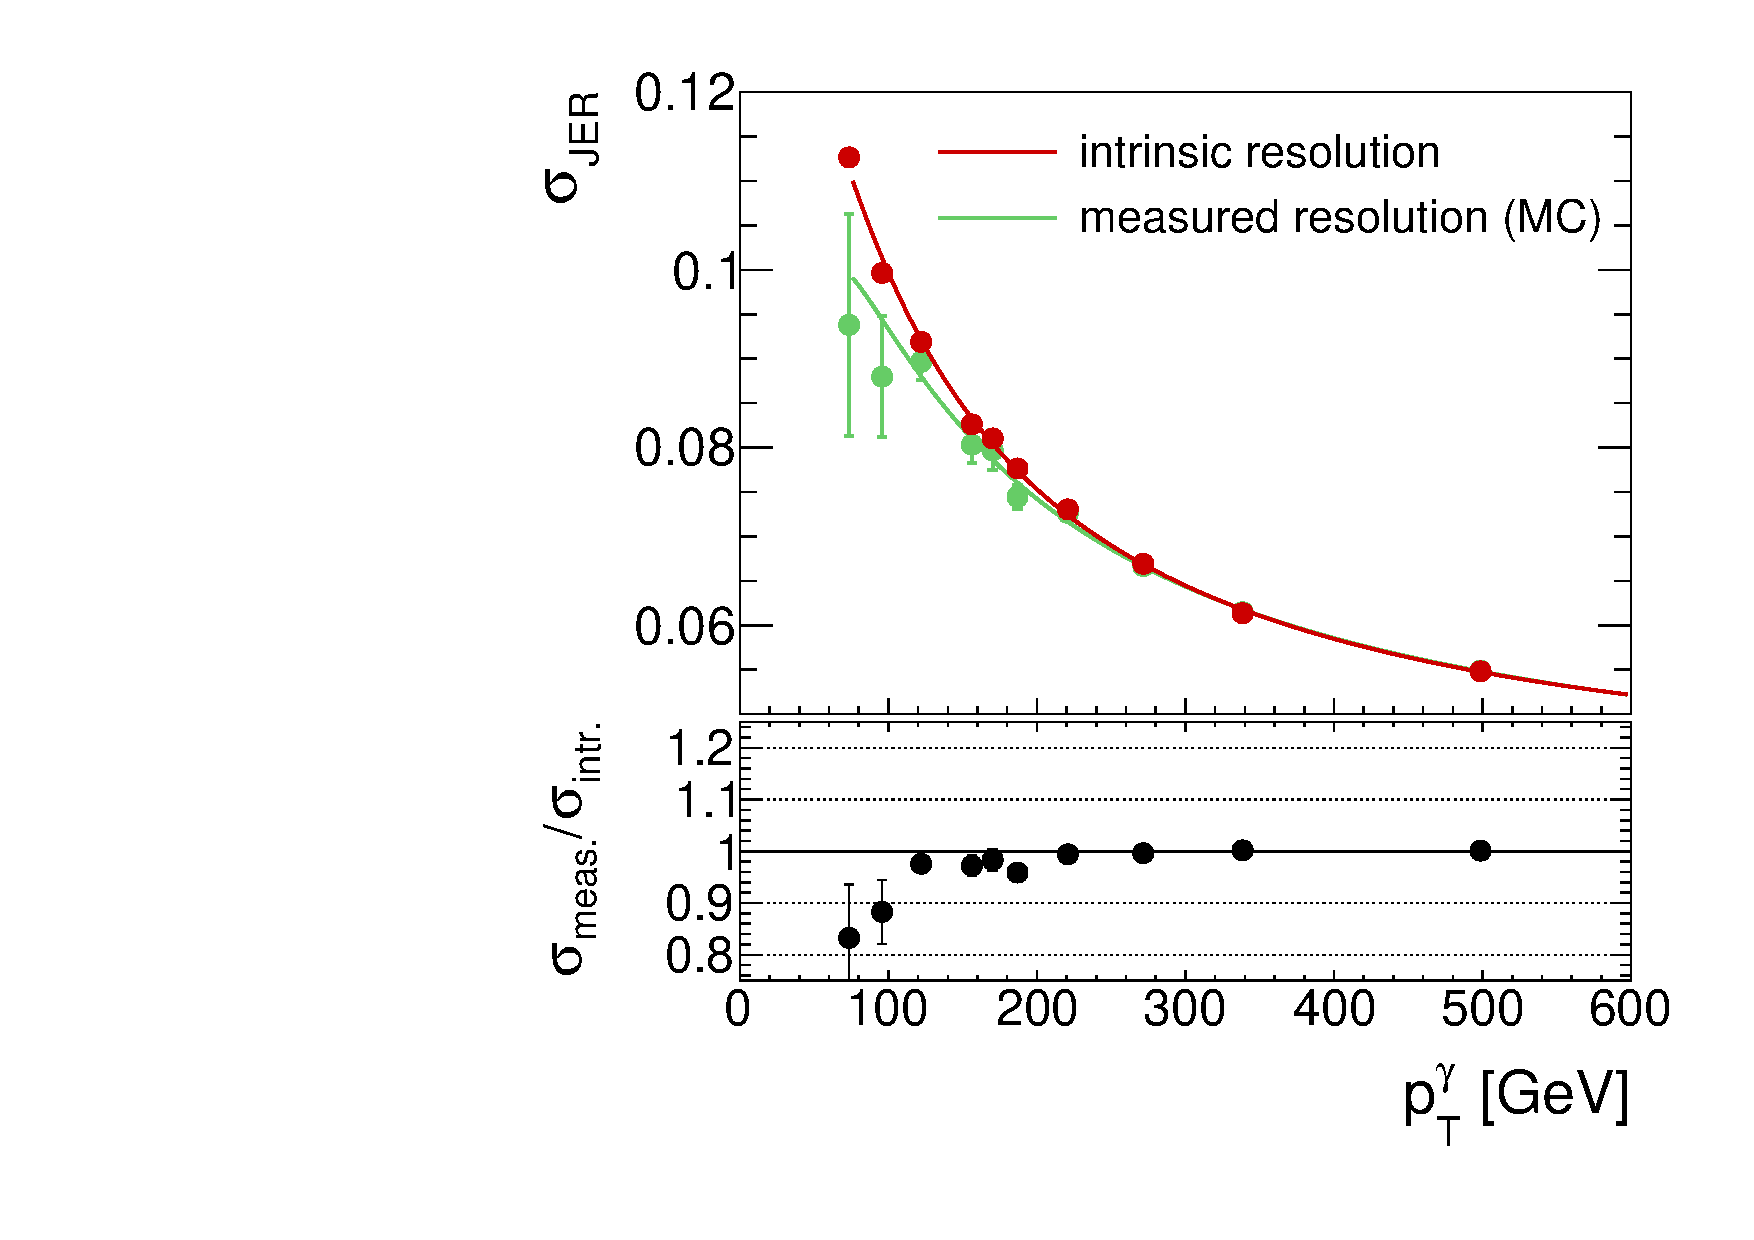
\includegraphics[width=0.49\textwidth]{figures/resolution/methodology/MCClosure_for_1_eta_bin_RMS99.pdf}
  \caption{Consistency check of the method: Comparison between \jer obtained from the measured resolution (Eq.~\eqref{eq:total}) and from the intrinsic resolution (Eq.~\eqref{eq:intrinsic}) in simulation.}  
  \label{fig:MCClosure}
\end{figure}
It can be seen that the method has a bias of up to~15\% towards an underestimation of the resolution for small \ptgamma. 
For $\ptgamma>100\gev$ the bias is less than 5\% and reduces to less than 1\% for $\ptgamma>200\gev$.

%It is evaluated as the ratio of the predicted intrinsic resolution by fitting Eq.~\eqref{eq:total} with $q$ fixed to the value obtained by Eq.~\eqref{eq:imbalance} over the intrinsic resolution directly obtained from the intrinsic response distribution \ptrecojet/\ptgenjet.

The residual bias of the method is caused by the accumulation of high \ptfirstjet events in the low alpha bins and low \ptfirstjet events in the high alpha bins.
Since the jet transverse-momentum resolution decreases for higher \ptfirstjet, this leads to an upward slope of the resolution with increasing alpha (cf. red dots in Fig~\ref{fig:AlphaDependenceOfResolutions} (left)).

The intrinsic resolution is not affected by this $\alpha$ dependency because it is fitted with a constant and thus corresponds to the mean resolution across all $\alpha$ bins.
In contrast, the fit of the measured resolution with an additional free parameter can adopt this increase and can therefore result in an underestimation of the y-intercept and thus of \jer. 
For high photon \pt, this effect is less pronounced, since the slope of \jer(\ptgamma) (see Fig.~\ref{fig:MCClosure}) flattens out. Thus the method is only biased for small \ptgamma.

The accumulation of high \ptfirstjet events in low $\alpha$~bins is stemming from two effects.
First, the binning in \ptgamma and the momentum balance between the photon and the first two jets lead to a dependency of the first jet \pt on the second jet \pt and therefore alpha: 
For a fixed \ptgamma, the \pt of the first jet gets smaller for larger \ptsecondjet in events where the second jet is in the leading jet hemisphere (see Fig.~\ref{fig:sketch}), 
leading to a dependency of $\ptfirstjet \propto -\ptsecondjet$.
This effect is directly opposite for events with a second jet in the photon hemisphere, where the first jet \pt gets larger for larger \ptsecondjet and thus $\ptfirstjet \propto \ptsecondjet$. 
%As the resolution of the jet improves with higher jet \pt (see Fig.~\ref{fig:ResolutionOfPtgamma}), a dependency of the leading jet \pt on the second jet \pt directly leads to a dependency of the intrinsic resolution on the second jet \pt. 
In principle, the effect should thus cancel out, but since the topology of a second jet in the leading jet hemisphere is much more frequent, a residual upward trend in the resolution vs. $\alpha$ is conserved. 

The second source of the accumulation of high \ptfirstjet events in low $\alpha$~bins arises from the alpha definition $\alpha = \ptsecondjet/\ptgamma$ and the non-zero width of the \ptgamma bins. 
Because of the inclusion of \ptgamma in $\alpha$ with $\alpha \propto 1/\ptgamma$, the high photon \pt events accumulate in the low alpha regions. 
As the selected events are almost balanced, a high \ptgamma is associated with a high jet \pt, thus also the high jet \pt events accumulate in the low alpha bins, leading to  an upward trend in the resolution vs. $\alpha$. \\
%This behaviour can be seen in the intrinsic resolution in Fig.~\ref{fig:AlphaDependenceOfResolutions}, where a small increase of the resolution to high $\alpha$ can be seen. 

However, since the discussed bias affects the resolution measurement in simulation and data equivalently, the residual bias for low \ptgamma is not of concern for the measurement of data-to-simulation resolution scale factors \rhores (Eq.~\eqref{res:eq:rhores}). 
%Hence, a possible bias in the separate resolution measurements for data and simulation should cancel out. 
To prove the hypothesis of a cancellation of the bias, a pseudo dataset is generated from the simulated dataset where the jet transverse-momentum resolution is smeared by $\rhores =1.1$ in all $|\etafirstjet|$ bins. 
Subsequently, the resolution scale factors between the smeared pseudo dataset and the original simulated dataset are determined according to the methodology presented in this thesis.
The resulting scale factors \rhores should reproduce the input values of $\rhores=1.1$.
In Fig.~\ref{res:fig:MCClosureRatio}, the result of this test is shown.
\begin{figure}[~t]
  \centering
    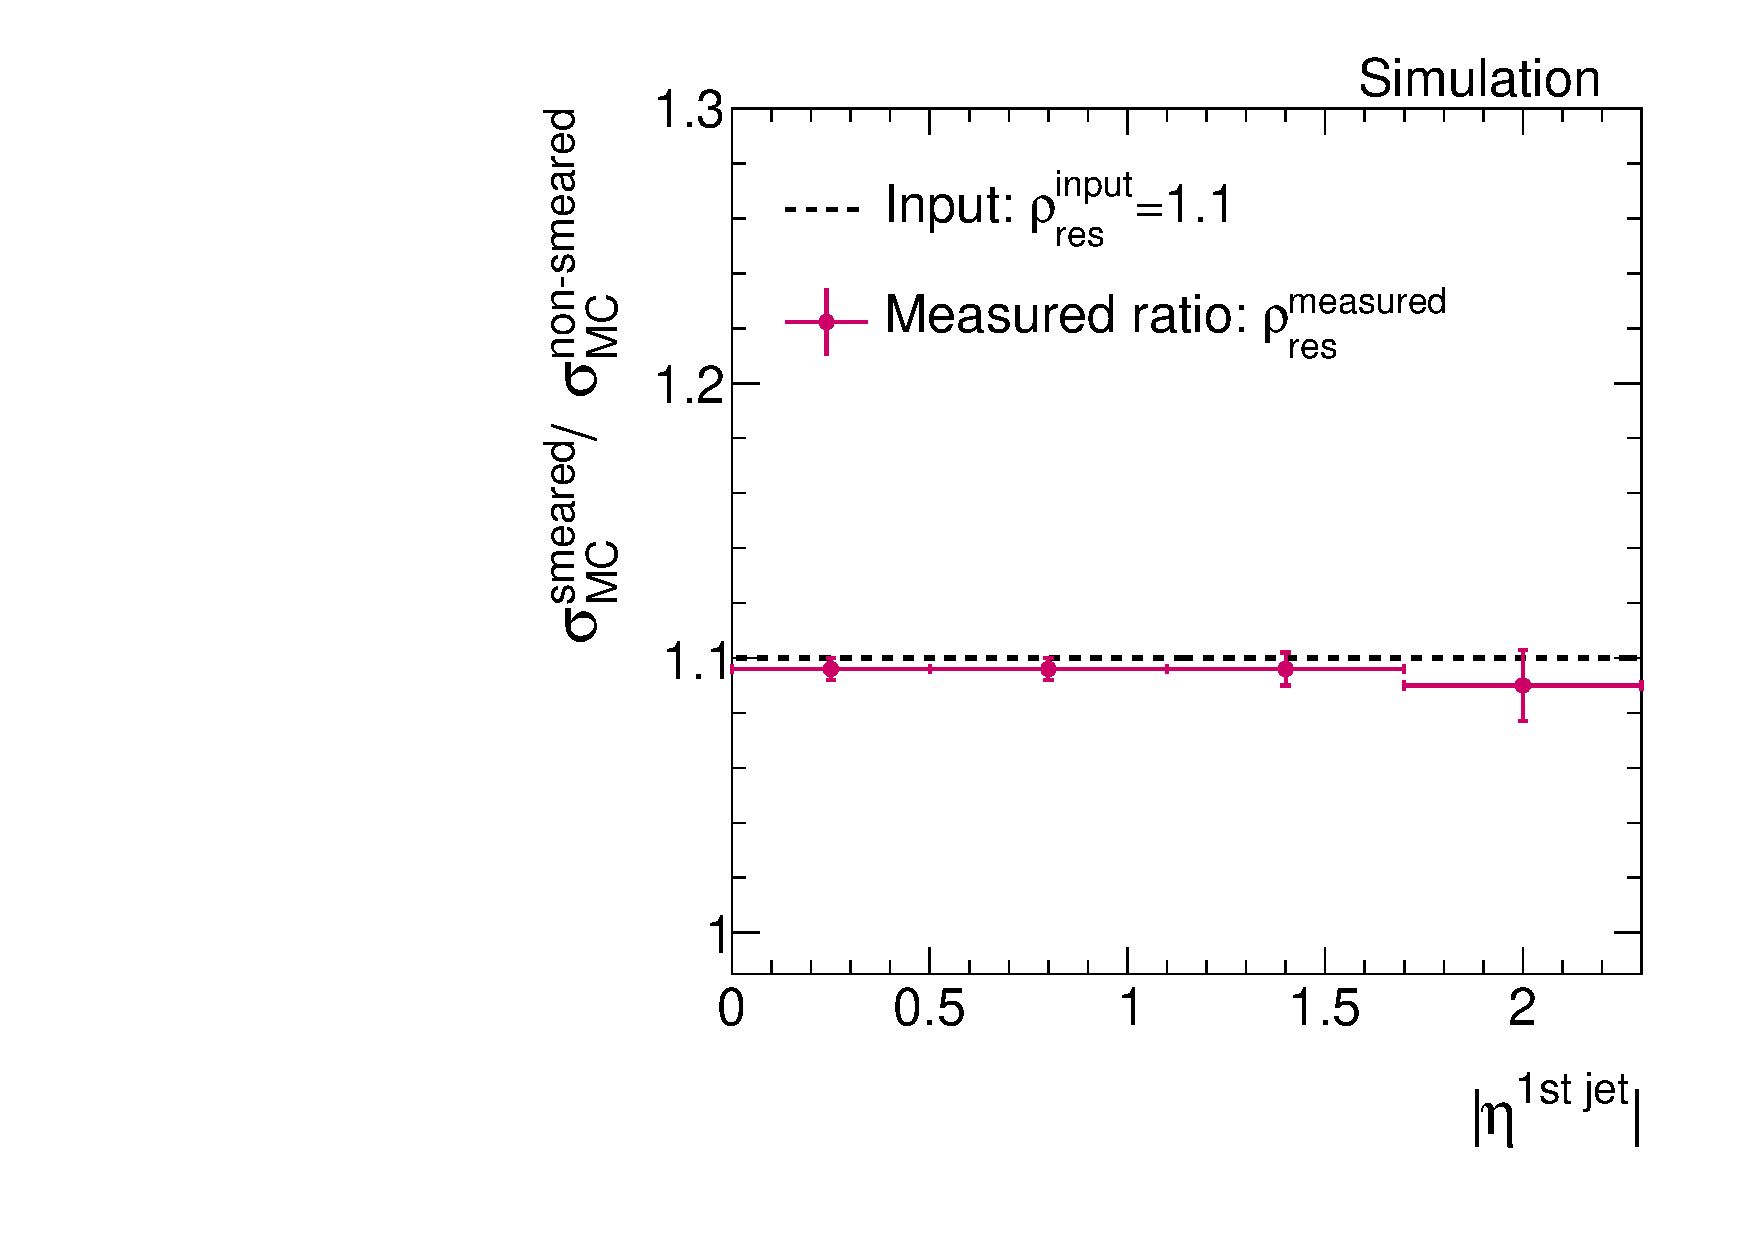
\includegraphics[width=0.49\textwidth]{figures/resolution/methodology/MCClosureRatio.pdf}
     \caption{Comparison of the resolution ratio $\jer^{\text{smeared MC}}/\jer^{\text{non-smeared MC}}$ measured in simulated events with the input smearing factor $\rhores=1.1$ in all four $|\etafirstjet|$ bins.}
  \label{res:fig:MCClosureRatio}
\end{figure}
In all $|\etafirstjet|$ bins, the measurement of the scale factors reproduces the input factors within the statistical uncertainties.
The deviation of the measured scale factors to the input value is less than 0.9\% in all four $|\etafirstjet|$ bins.
Thus, the method is expected to also hold for the determination of the data-to-simulation ratio.

After the characterisation and estimation of the associated systematic uncertainties of the jet transverse-momentum resolution measurement with \GAMJET events, the results of the measurement on $\sqrt{s}=8\tev$ data will be presented.
%%%%%%%%%%%%%%%%%%%%%%%%%%%%%%%%%%%%%%%%%%%%%%%%%%%%%%%%%%%%%%%%%%%%%%%%%%%%%%%%%%%%%%%%%%%%%%%%%%%%%%%%%%%%%%%%%%%%%%%%%%%%%%%%%%%%%%%%%%%%%%%%%%%%%%%%%%%%%%%%%%%%%%%%%%%%%%%%%%%%%%%%%%%%%%%%%%%%%%%%%%%%%%%%%%%%%%%%%%%%%%%%%%%
%%%%%%%%%%%%%%%%%%%%%%%%%%%%%%%%%%%%%%%%%%%%%%%%%%%%%%%%%%%%%%%%%%%%%%%%%%%%%%%%%%%%%%%%%%%%%%%%%%%%%%%%%%%%%%%%%%%%%%%%%%%%%%%%%%%%%%%%%%%%%%%%%%%%%%%%%%%%%%%%%%%%%%%%%%%%%%%%%%%%%%%%%%%%%%%%%%%%%%%%%%%%%%%%%%%%%%%%%%%%%%%%%%%
%%%%%%%%%%%%%%%%%%%%%%%%%%%%%%%%%%%%%%%%%%%%%%%%%%%%%%%%%%%%%%%%%%%%%%%%%%%%%%%%%%%%%%%%%%%%%%%%%%%%%%%%%%%%%%%%%%%%%%%%%%%%%%%%%%%%%%%%%%%%%%%%%%%%%%%%%%%%%%%%%%%%%%%%%%%%%%%%%%%%%%%%%%%%%%%%%%%%%%%%%%%%%%%%%%%%%%%%%%%%%%%%%%%
\FloatBarrier
\chapter{Systematic uncertainties}

Many systematic uncertainties of the jet transverse-momentum resolution measurement cancel out when focusing on the data-to-simulation ratio $\jer^{\text{data}}/\jer^{\text{MC}}$.
In the following subsections, only uncertainties relevant for this ratio will be discussed.

For the final uncertainty, the single uncertainties are added in quadrature, resulting in relative uncertainties between 2.3\% to 6.3\% for the lowest and highest $|\etafirstjet|$ bin, respectively. 

An overview of all systematic uncertainties can be found in Table~\ref{res:tab:Uncertainties}.

\renewcommand{\arraystretch}{1.1}
\begin{table}[h]
\centering
\caption{All relative systematic uncertainties on the data-to-simulation ratio $\jer^{\text{data}}/\jer^{\text{MC}}$ listed by sources for the different $|\eta^{\text{jet}}|$ bins.}
\label{res:tab:Uncertainties}
\makebox[0.99\textwidth]{
\begin{tabular}{l  c  c  c  c}
\multicolumn{5}{c}{} \\
\toprule
\multicolumn{1}{c}{} & \multicolumn{4}{c}{$|\etajet|$}\\
\multicolumn{5}{c}{} \\
& \textbf{0.0 - 0.5}& \textbf{0.5 - 1.1}& \textbf{1.1 - 1.7}& \textbf{1.7 - 2.3}\\
\midrule
\multirow{2}{*}{\textbf{Multijet contamination}}& $+2.0 \% $ & $+2.0 \% $ & $+2.3 \% $ & $+2.5 \% $ \\
                                                & $-2.0 \% $ & $-2.0 \% $ & $-2.3 \% $ & $-2.5 \% $ \\
\multicolumn{5}{c}{} \\
\multirow{2}{*}{\textbf{Simulation of flavor composition}}& $+0.9 \% $ & $+0.9 \% $ & $+0.8 \% $ & $+0.6 \% $ \\
& $-0.9 \% $ & $-0.9 \% $ & $-0.8 \% $ & $-0.6 \% $ \\
\multicolumn{5}{c}{} \\
\multirow{2}{*}{\textbf{Simulation of out-of-cone showering}}& $+0.5 \% $ & $+2.8 \% $ & $+3.6 \% $ & $+5.7 \% $ \\
& $-0.5 \% $ & $-2.8 \% $ & $-3.6 \% $ & $-5.7 \% $ \\
\multicolumn{5}{c}{} \\
\multirow{2}{*}{\textbf{Jet energy scale}}& $+0.6 \% $ & $+0.6 \% $ & $+0.6 \% $ & $+0.7 \% $ \\
& $-0.5 \% $ & $-0.6 \% $ & $-0.6 \% $ & $-0.6 \% $ \\
\multicolumn{5}{c}{} \\
\multirow{2}{*}{\textbf{Pileup reweighting}}& $+0.1 \% $ & $+0.1 \% $ & $+0.1 \% $ & $+0.2 \% $ \\
& $-0.1 \% $ & $-0.1 \% $ & $-0.2 \% $ & $-0.2 \% $ \\
\midrule
\multirow{2}{*}{\textbf{Total}}& $+2.3 \% $ & $+3.6 \% $ & $+4.4 \% $ & $+6.3 \% $ \\
& $-2.3 \% $ & $-3.6 \% $ & $-4.4 \% $ & $-6.3 \% $ \\
\bottomrule
\multicolumn{5}{c}{} \\
\end{tabular}}
\end{table} 

%%%%%%%%%%%%%%%%%%%%%%%%%%%%%%%%%%%%%%%%%%%%%%%%%%%%%%%%%%%%%%%%%%%%%%%%%%%%%%%%%%%%%%%%%%%%%%%%%%%%%%%%%%%%%%%%%%%%%%%%%%%%%%%%%%%%%%%%%%%%%%%%%%%%%%%%%%%%%%%%%%%%%%%%%%%%%%%%%%%%%%%%%%%%%%%%%%%%%%%%%%%%%%%%%%%%%%%%%%%%%%%%%%%
\section*{Uncertainty on the contamination with QCD-multijet events}
Due to the huge QCD-multijet cross section, a countable fraction of dijet events can survive the strict photon selection (see Section~\ref{subsec:PhotonSelection}) if a jet is misidentified as a photon.
This happens, when \eg a jet hadronises to a $\pi^0$ that decays to two photons that mimic the signature of an isolated photon from a $\GAMJET$ event.

The two leading jets in a dijet event are balanced except for initial and final state radiation and have in principle the same topology as \GAMJET events.
Therefore, the presented method is in principle insensitive to dijet contamination.
Adverse effects of dijet background contamination are only expected due to a mismeasurement of the \pt of the jet misidentified as photon, because only the energy of the $\pi^0$ is counted and not the full jet energy.
Another aspect is the different flavor composition of a QCD-multijet sample. 
Due to the different production mechanism, QCD-dijets are predominantly initiated by gluons while the leading jet in $\GAMJET$ events often stems from a light quark.
The number of particles after hadronisation is typically larger for gluon jets, hence the single particles are less energetic and out-of-cone showering is more pronounced.
Since the residual imbalance~$q$ in this analysis is taken from simulation considering \GAMJET events only, it is not expected to accurately describe the residual imbalance in the data sample that is contaminated with dijet events.

To investigate the impact of QCD-multijet contamination, a QCD-multijet sample, enriched in jets with a large electromagnetic fraction, is added to the \GAMJET sample and weighted according to the cross section.
Subsequently, the resolution measured using both the \GAMJET and the QCD-multijet sample is compared to the resolution measured with the \GAMJET sample only.
Since the QCD-multijet sample has very large event weights leading to high statistical uncertainties on the measured jet transverse-momentum resolution, two selection criteria ($\alpha<0.4$ and $\Delta\Phi>2.7$) are relaxed in order to increase the statistical precision of the uncertainty estimation.
Additionally, a rougher binning in $\alpha$, \ptgamma and $|\etafirstjet|$ is applied.
The residual imbalance~$q$ of the resolution measurement including the QCD-multijet sample is fixed to the residual imbalance determined from the \GAMJET only analysis in order to account for a possible error in the evaluation of the $\jer^{\text{data}}/\jer^{\text{MC}}$ ratio for which data is only compared to a \GAMJET sample.
It can be seen from Fig.~\ref{res:fig:QCDuncertainty} that the jet transverse-momentum resolution is worse for low \ptgamma when considering QCD-multijet contamination.
\begin{figure}[!b]
  \centering
      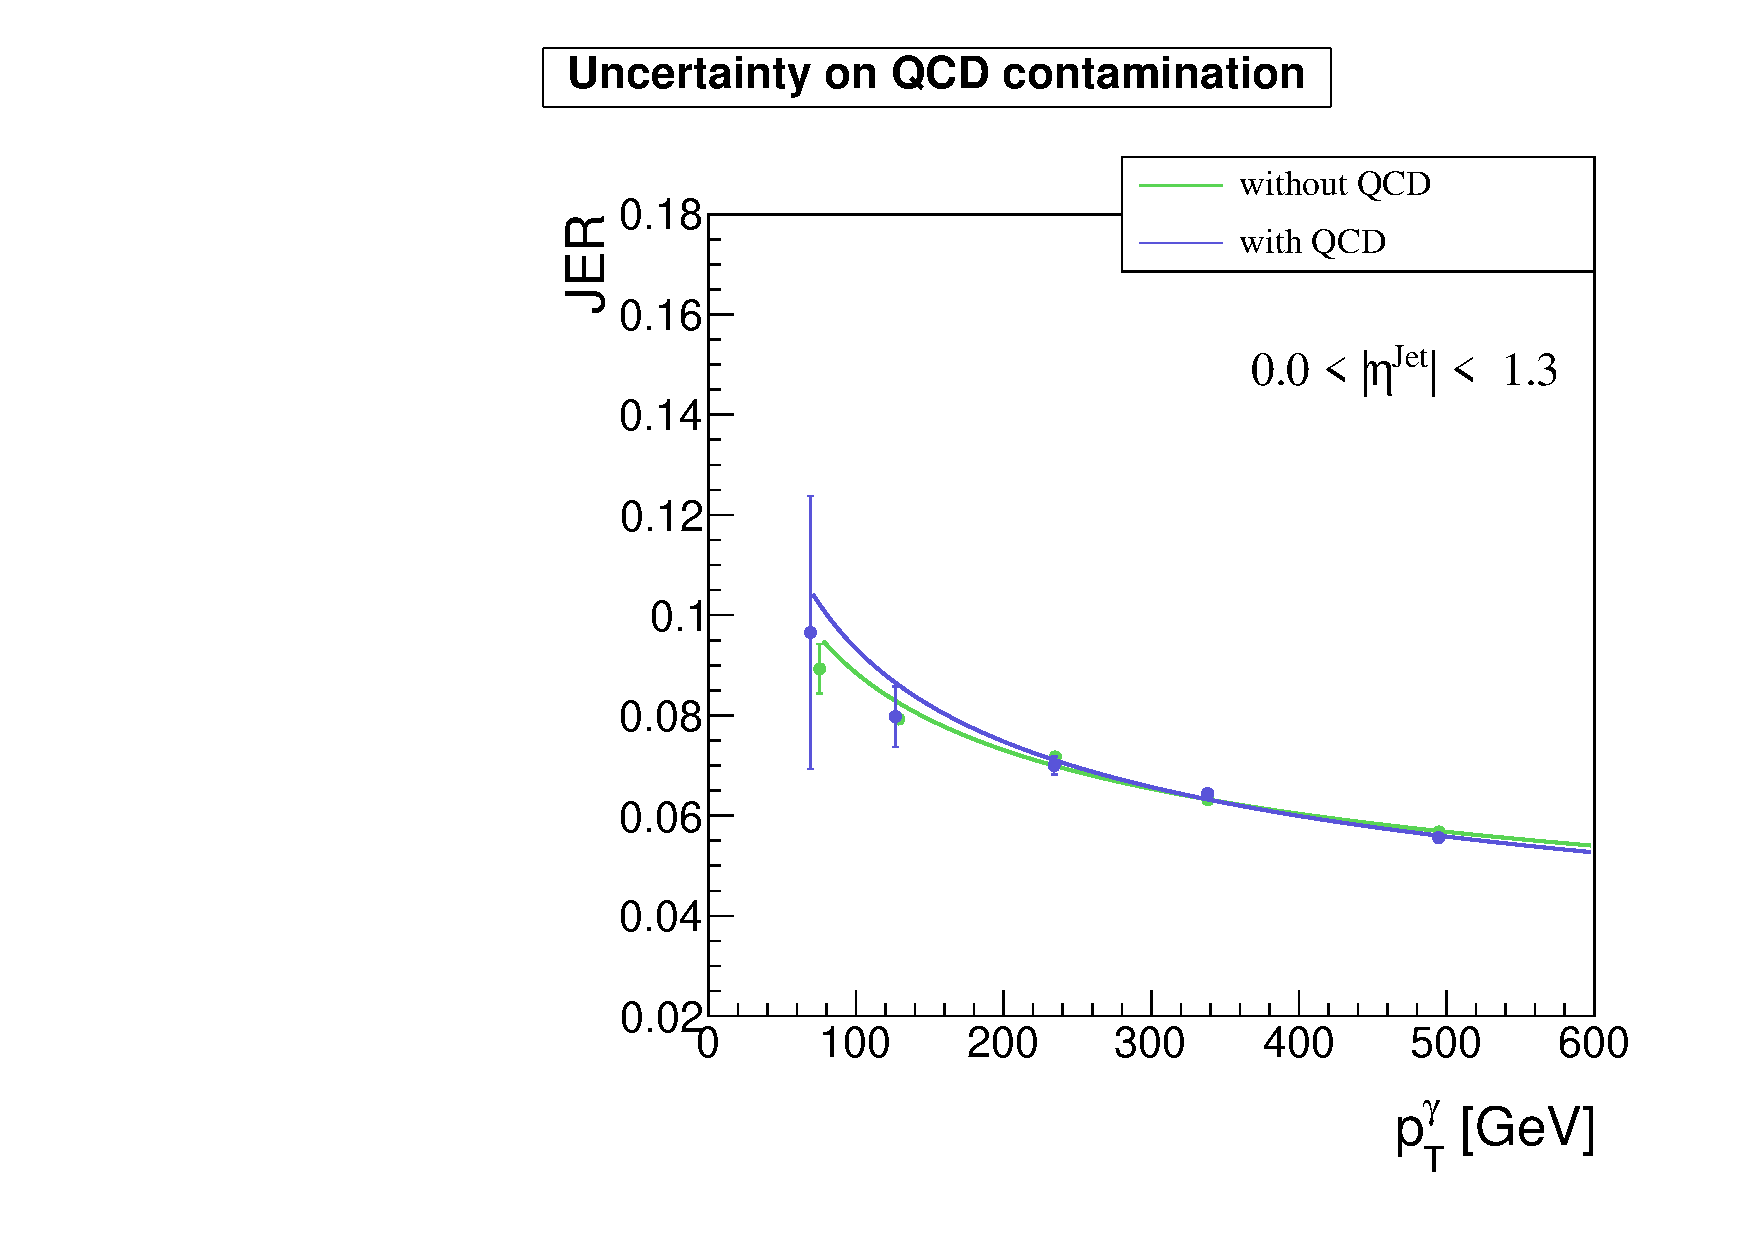
\includegraphics[width=0.49\textwidth]{figures/resolution/systematicUncertainties/Resolution_for_1_eta_bin_QCDUncertainty_RMS99.pdf}
  \caption{The jet transverse-momentum resolution measured in simulation for $|\etafirstjet| < 1.3$ with (blue) and without (green) a QCD-multijet sample added to the \GAMJET sample.}  
  \label{res:fig:QCDuncertainty}
\end{figure}

The impact on the data-to-simulation ratio is estimated by adding the QCD-multijet sample on top of the simulated \GAMJET sample and redoing the evaluation of the scale factors.
The resulting uncertainties vary between $2.0-2.5\%$ for the different $|\etafirstjet|$ regions (cf. Table~\ref{res:tab:Uncertainties}).

\section*{Uncertainty on the flavor composition in simulation}
A possible difference between the resolution of different jet flavors (\eg caused by more pronounced out-of-cone showering of gluon jets) should in principle not play a role for the data-to-simulation scale factors \rhores as long as the flavor composition in data and simulation is the same.

To account for possible discrepancies in the flavor composition between data and simulation, the gluon and quark flavor fractions of the simulated sample (Fig~\ref{res:fig:FlavorFraction}) are varied by 10\%.
\begin{figure}[!b]
  \centering
      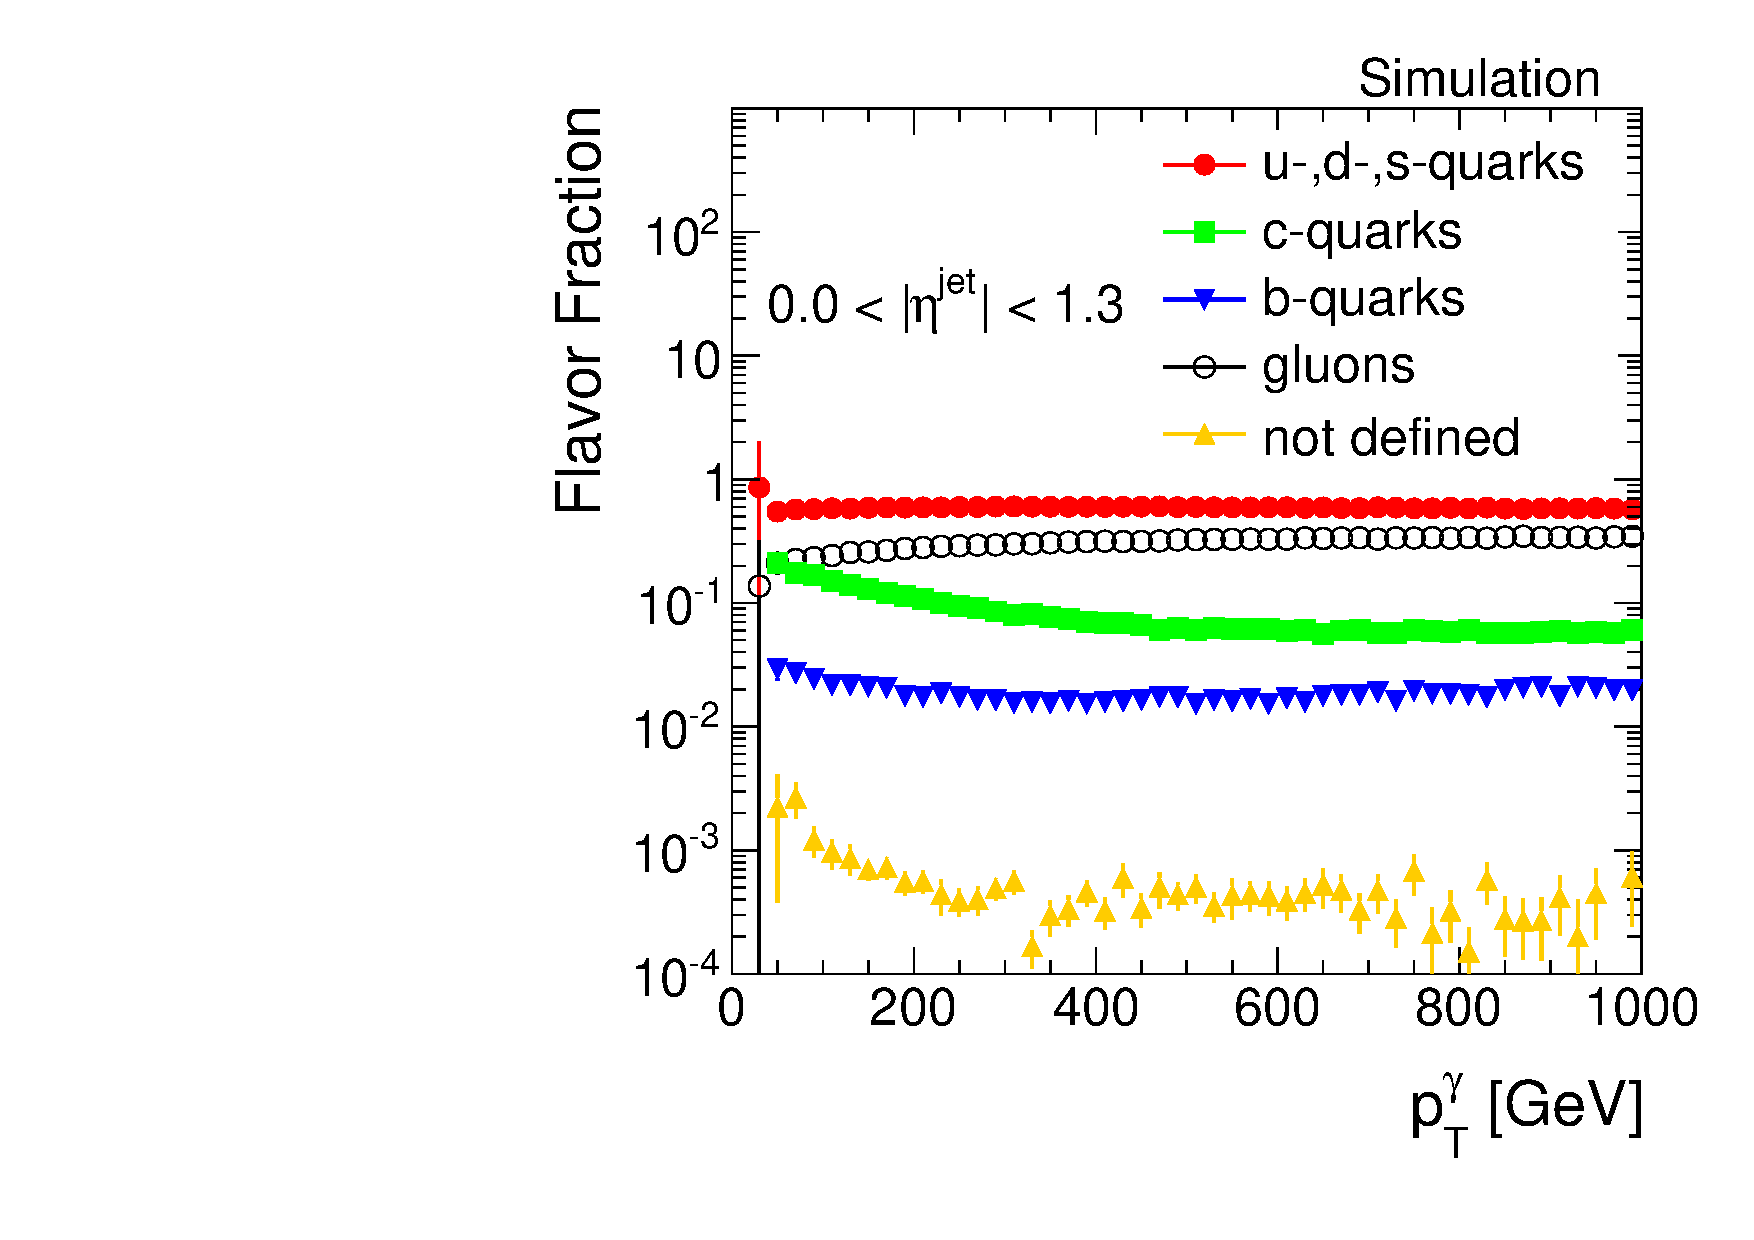
\includegraphics[width=0.49\textwidth]{figures/resolution/systematicUncertainties/flavorFraction_barrel_algo.pdf}
  \caption{The flavor composition in the simulated \GAMJET sample in the barrel region of the detector. The ``algorithmic'' flavor definition is used (see Appendix~\ref{res:app:FlavorDefinition} for more details).}  
  \label{res:fig:FlavorFraction}
\end{figure}
To estimate the effect of different flavour compositions, the resolution in simulation is separately evaluated for quarks ($\jer^\text{quarks}$) and gluons ($\jer^\text{gluons}$). 

There are various definitions used in the CMS collaboration how to assign the underlying generator-level quark/gluon flavor to a jet.
In this measurement the so-called ``algorithmic'' flavor definition is used which classifies b- or c-jets from gluon splitting as b- or c-quarks (see Appendix~\ref{res:app:FlavorDefinition} for more details on this definition).
The composition in the simulated \pythia \GAMJET sample is around 60\% light quarks and 20\% to 35\% gluons (see Fig.~\ref{res:fig:FlavorFraction}). 
The missing fraction is mainly made up out of charm quarks. 


The left panel of Figure~\ref{res:fig:ResolutionDifferences} depicts the intrinsic resolution for all flavors separately for $|\etafirstjet|<1.3$.
\begin{figure}[!t]
  \centering
      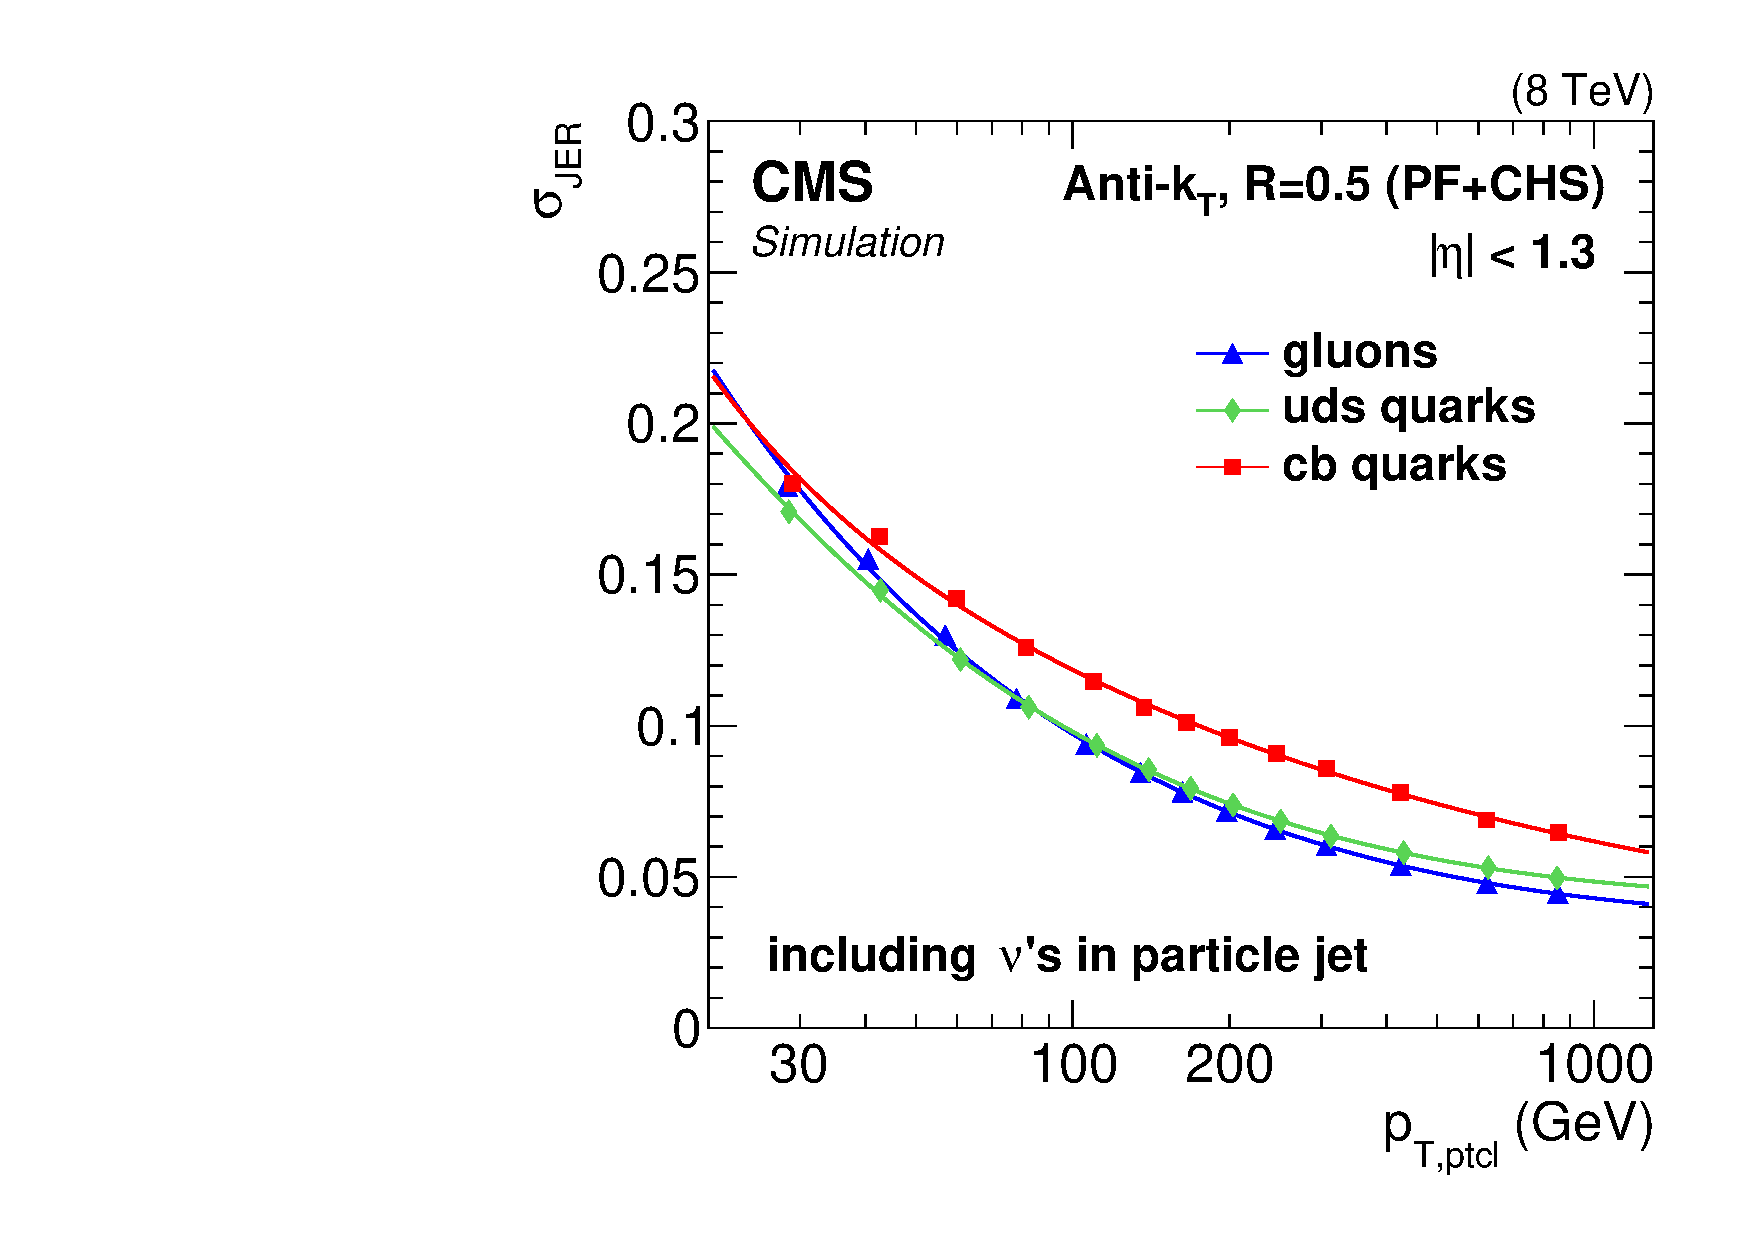
\includegraphics[width=0.49\textwidth]{figures/resolution/systematicUncertainties/Figure_38_withNu_Teresa_updated_4.pdf}
      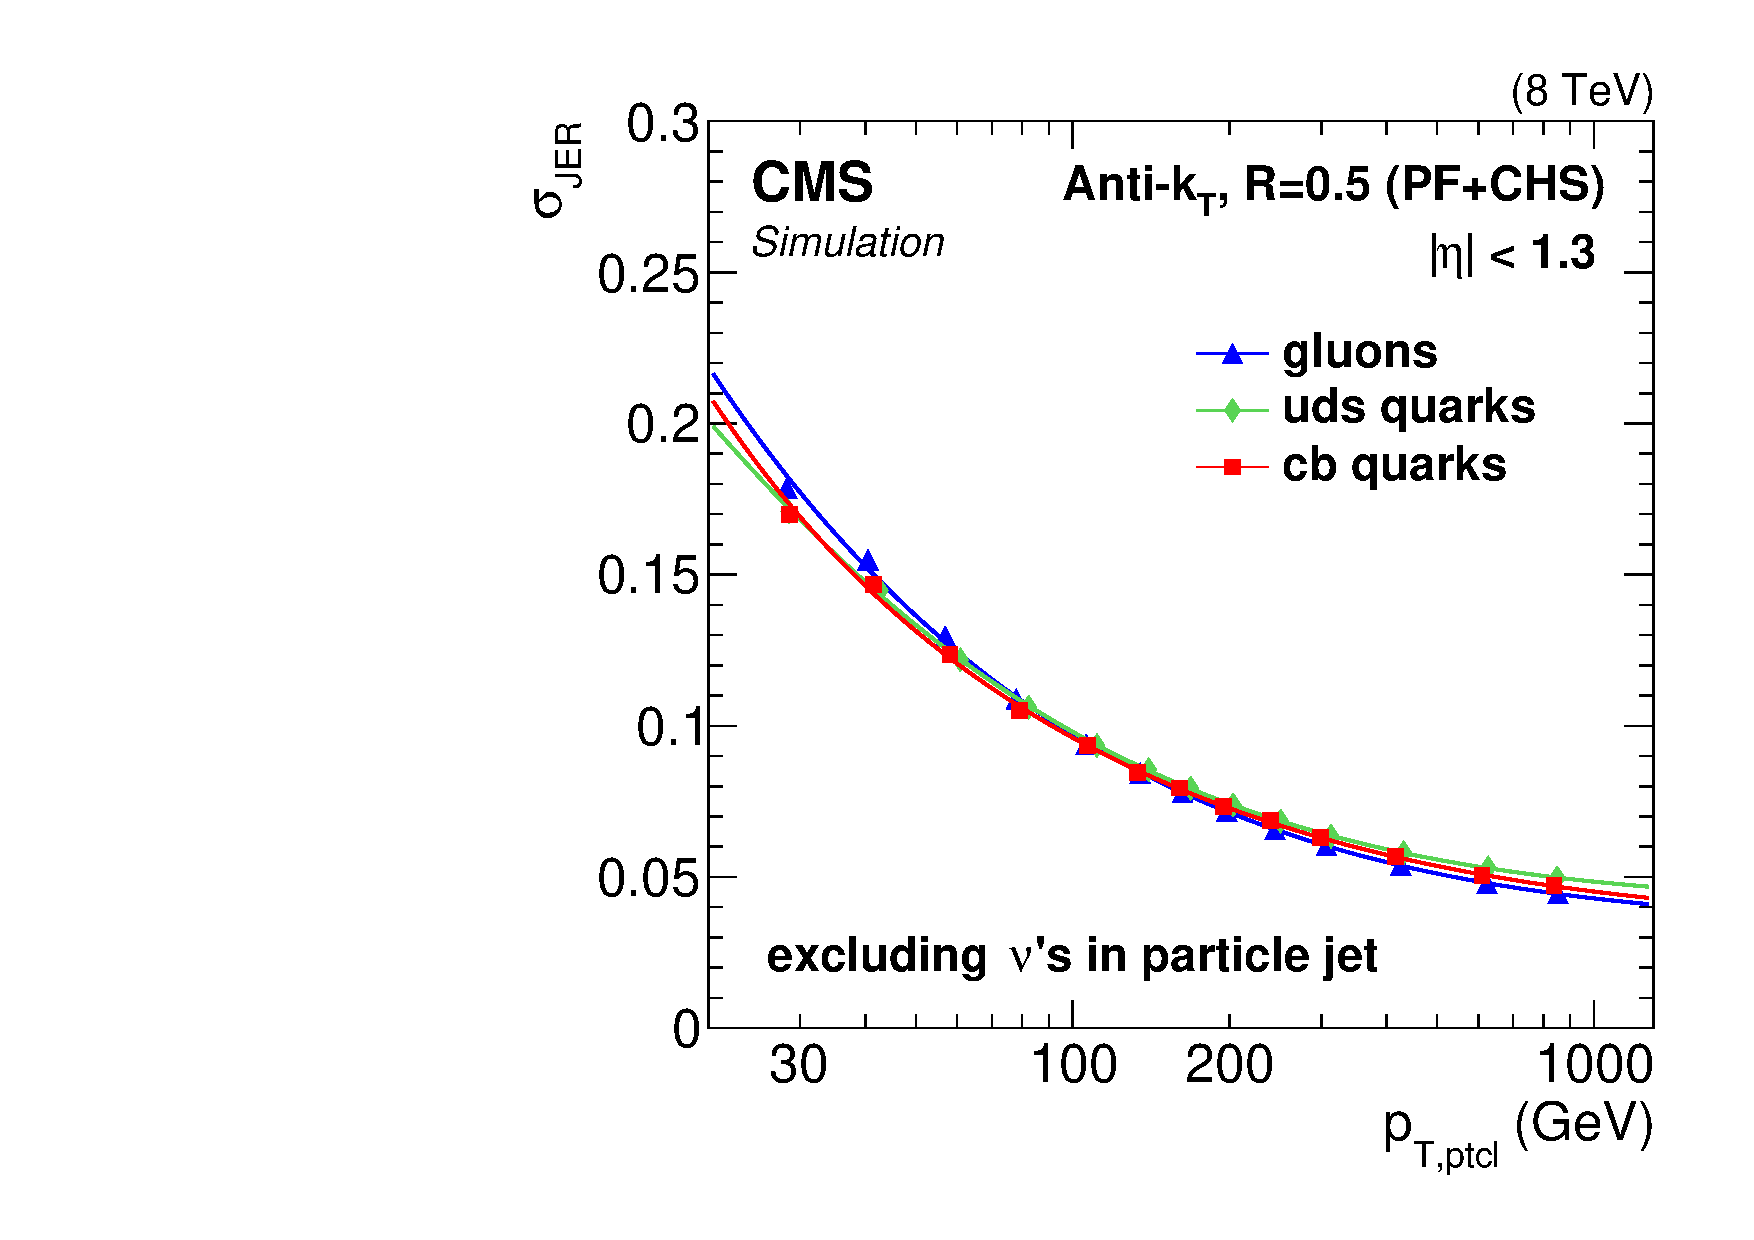
\includegraphics[width=0.49\textwidth]{figures/resolution/systematicUncertainties/Figure_38_noNu_Teresa_updated_4.pdf}
      %\includegraphics[width=0.49\textwidth]{figures/resolution/systematicUncertainties/Figure_39_withNu_Teresa_updated_3.pdf}
      %\includegraphics[width=0.49\textwidth]{figures/resolution/systematicUncertainties/Figure_39_noNu_Teresa_updated_3.pdf}
  \caption{The intrinsic resolution \jerintr for $|\etafirstjet| < 1.3$ for different jet flavors with (left) and without (right) including the neutrinos in the generator-level jet.
           Here, JER refers to \jerintr, and $p_{\text{T,\,ptcl}}$ to the generator-level jet \pt. }  
  \label{res:fig:ResolutionDifferences}
\end{figure}
It can be seen that the resolution for gluon and light quark jets is comparable whereas heavier quarks have a worse resolution across the full \pt range.
This is because the decay of heavy quarks can involve the production of neutrinos, whose transverse momentum is not detectable, leading to an underestimation of the reconstructed jet \pt.
Since the neutrino \pt is included in the jet \pt on generator level, c- and b-jets have a more pronounced left tail of the jet transverse-momentum response, leading to a worse resolution compared to light quark jets (left part of Fig.~\ref{res:fig:ResolutionDifferences}). 
This is not the case, if the neutrino \pt is not added to the generator-level jet \pt, as can be seen in Fig~\ref{res:fig:ResolutionDifferences} (right).
%However, for the here presented measurement is does not play a role whether the neutrino \pt is added to the generator-level jet \pt, because in case it is not included into the intrinsic response the long left tail of the response function for b- and c-quarks is then transferred to the imbalance response.
%Thus, the right tail of b- and c-quarks does anyway enter the jet transverse-momentum resolution measurement with \GAMJET events, either in the intrinsic or in the imbalance response.

In order to estimate the uncertainty, the flavor composition in simulation is varied by 10\% and the weighted mean of the quark and the gluon resolution is calculated.
Finally, the constant fit to the data-to-simulation ratio $\jer^{\text{data}}/\jer^{\text{MC}}$ is reevaluated, leading to a final systematic uncertainty between $0.6-0.9\%$.

%%%%%%%%%%%%%%%%%%%%%%%%%%%%%%%%%%%%%%%%%%%%%%%%%%%%%%%%%%%%%%%%%%%%%%%%%%%%%%%%%%%%%%%%%%%%%%%%%%%%%%%%%%%%%%%%%%%%%%%%%%%%%%%%%%%%%%%%%%%%%%%%%%%%%%%%%%%%%%%%%%%%%%%%%%%%%%%%%%%%%%%%%%%%%%%%%%%%%%%%%%%%%%%%%%%%%%%%%%%%%%%%%%%
\section*{Uncertainty on the simulation of out-of-cone showering}
Another source of uncertainty is the use of information from Monte Carlo simulation by determining the residual imbalance $q$ from the simulated \GAMJET sample (Eq.~\eqref{eq:total}).

Since it cannot be expected that out-of-cone showering is well modelled in simulation, possible differences between real and simulated out-of-cone showering are estimated by the evaluation of the ratio $\jer^{\text{data}}/\jer^{\text{MC}}$ using different jet radii of the jet reconstruction algorithm. 

For the primary analysis, jets reconstructed by the Anti-k$_{\text{t}}$ algorithm with a radius of $R=0.5$ are used (AK5-jets). 
In order to evaluate the systematic uncertainty on the out-of-cone showering simulation, the measurement of \rhores redone with jets reconstructed with a jet radius of $R=0.7$ (AK7-jets). 

The data-to-simulation ratio is in all $|\etafirstjet|$ bins larger for AK7-jets, resulting in uncertainties between $0.5-5.7\%$.
The uncertainty on the simulation of out-of-cone showering is thus the largest systematic uncertainty of this measurement.



%%%%%%%%%%%%%%%%%%%%%%%%%%%%%%%%%%%%%%%%%%%%%%%%%%%%%%%%%%%%%%%%%%%%%%%%%%%%%%%%%%%%%%%%%%%%%%%%%%%%%%%%%%%%%%%%%%%%%%%%%%%%%%%%%%%%%%%%%%%%%%%%%%%%%%%%%%%%%%%%%%%%%%%%%%%%%%%%%%%%%%%%%%%%%%%%%%%%%%%%%%%%%%%%%%%%%%%%%%%%%%%%%%%
\section*{Uncertainty on the jet energy scale}
A further uncertainty arises from the correction of the jet energy scale.
The transverse momentum of each jet is corrected in order to have uniform response over the full $\eta^{\text{jet}}$, and $\pt^{\text{jet}}$ range~\cite{bib:CMS:JME_PAS}.
In simulation, it is additionally corrected to account for data-simulation differences.
The latter correction can be a important for the evaluation of the data-to-simulation ratio.
Thus, the uncertainties on the correction factors that are only applied to the simulated samples are varied up and down within their $1\sigma$-uncertainties.

The effect of the jet \pt variation on the data-to-simulation ratio is of minor importance and range between $0.5-0.7\%$.


%%%%%%%%%%%%%%%%%%%%%%%%%%%%%%%%%%%%%%%%%%%%%%%%%%%%%%%%%%%%%%%%%%%%%%%%%%%%%%%%%%%%%%%%%%%%%%%%%%%%%%%%%%%%%%%%%%%%%%%%%%%%%%%%%%%%%%%%%%%%%%%%%%%%%%%%%%%%%%%%%%%%%%%%%%%%%%%%%%%%%%%%%%%%%%%%%%%%%%%%%%%%%%%%%%%%%%%%%%%%%%%%%%%%%%%%%%%
\section*{Uncertainty on the pileup reweighting}
Finally, an uncertainty due to the adjustment of the simulated events to the pileup distribution in data is evaluated.

To account for this uncertainty, the effect of a 5.0\% up- and downward variation of the minimum-bias cross section (69.4\,mb) on the resolution is evaluated, following the recommended procedure from~\cite{bib:CMS:PileupSysUnc}.
The resulting uncertainties are almost negligible and ranges between $0.1-0.2\%$.
%%%%%%%%%%%%%%%%%%%%%%%%%%%%%%%%%%%%%%%%%%%%%%%%%%%%%%%%%%%%%%%%%%%%%%%%%%%%%%%%%%%%%%%%%%%%%%%%%%%%%%%%%%%%%%%%%%%%%%%%%%%%%%%%%%%%%%%%%%%%%%%%%%%%%%%%%%%%%%%%%%%%%%%%%%%%%%%%%%%%%%%%%%%%%%%%%%%%%%%%%%%%%%%%%%%%%%%%%%%%%%%%%%%

%%%%%%%%%%%%%%%%%%%%%%%%%%%%%%%%%%%%%%%%%%%%%%%%%%%%%%%%%%%%%%%%%%%%%%%%%%%%%%%%%%%%%%%%%%%%%%%%%%%%%%%%%%%%%%%%%%%%%%%%%%%%%%%%%%%%%%%%%%%%%%%%%%%%%%%%%%%%%%%%%%%%%%%%%%%%%%%%%%%%%%%%%%%%%%%%%%%%%%%%%%%%%%%%%%%%%%%%%%%%%%%%%%%
%%%%%%%%%%%%%%%%%%%%%%%%%%%%%%%%%%%%%%%%%%%%%%%%%%%%%%%%%%%%%%%%%%%%%%%%%%%%%%%%%%%%%%%%%%%%%%%%%%%%%%%%%%%%%%%%%%%%%%%%%%%%%%%%%%%%%%%%%%%%%%%%%%%%%%%%%%%%%%%%%%%%%%%%%%%%%%%%%%%%%%%%%%%%%%%%%%%%%%%%%%%%%%%%%%%%%%%%%%%%%%%%%%%
\FloatBarrier
\chapter{Results}
\label{res:ch:results}

The data-to-simulation resolution scale factors \rhores are determined in $19.7\fbinv$ of $pp$-collision data at $\sqrt{s} = 8 \tev$ with the methodology described in Chapter~\ref{res:ch:methodology}.
In each $\alpha$-, \ptgamma- and $|\etafirstjet|$-bin, the width of the 99\% truncated response histogram is determined in simulation and data.
Afterwards, the extrapolation to zero additional jet activity is carried out, by fixing the imbalance $q$ in simulation and in data to the value extracted from the imbalance extrapolation in simulation.
Exemplary extrapolations for the imbalance, the intrinsic and the measured resolution in simulation and the measured resolution in data are shown in Fig.~\ref{res:fig:ExtrapolationsWithData}.
\begin{figure}[!t]
 \centering
    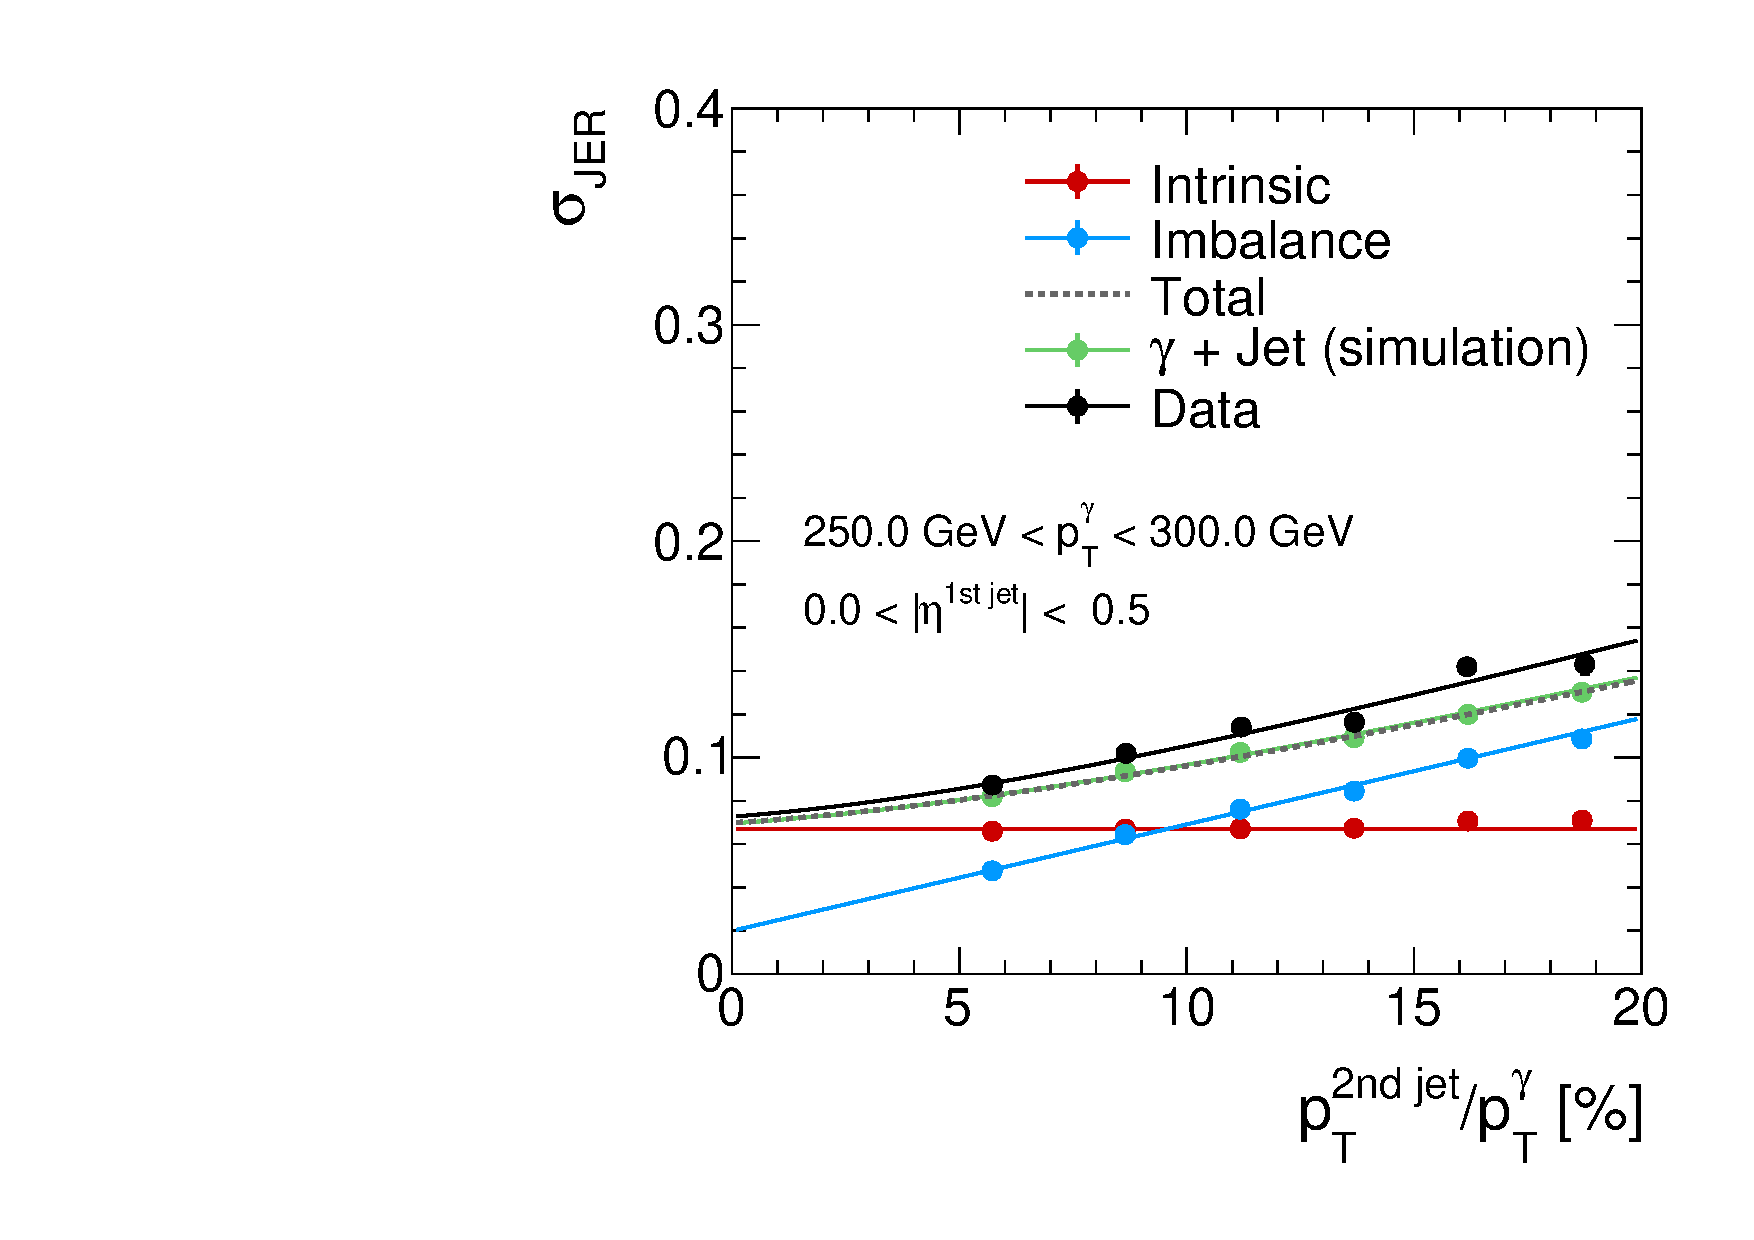
\includegraphics[width=0.49\textwidth]{figures/resolution/results/JER_for_1_eta_bin_10_pTGamma_bin_all_contributions_PFCHS_RMS99_mc.pdf}
    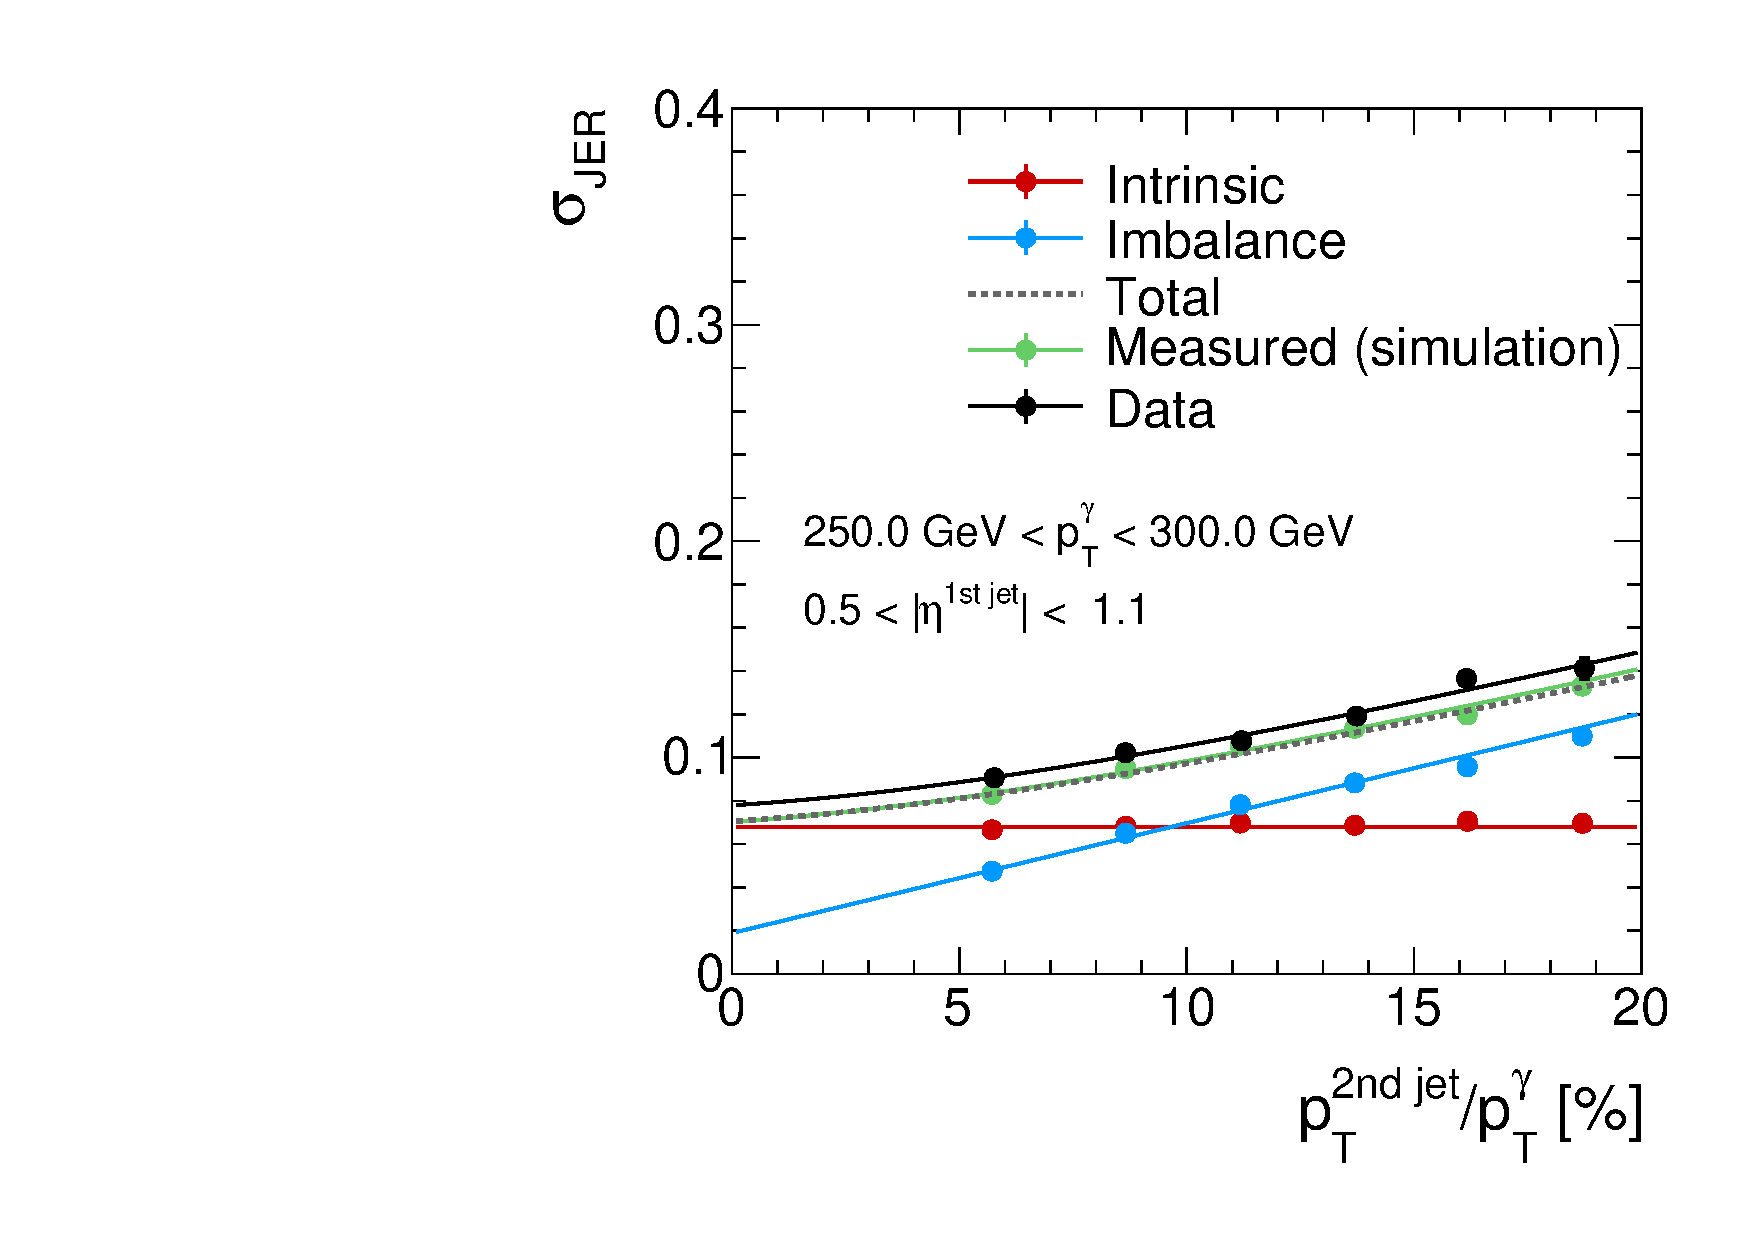
\includegraphics[width=0.49\textwidth]{figures/resolution/results/JER_for_2_eta_bin_10_pTGamma_bin_all_contributions_PFCHS_RMS99_mc.pdf}
  \caption{Two examples of the alpha dependency of the measured jet transverse-momentum resolution in data (black dots), in simulation (green dots) and  of the intrinsic (red dots) and the imbalance (blue dots) part 
           of the resolution in simulated events. All resolutions are fitted with the corresponding functions introduced in Chapter~\ref{res:ch:methodology} (Eqs.~\eqref{eq:intrinsic}-~\eqref{eq:total}).
           The total resolution (grey dotted line) is the addition in quadrature of the imbalance (blue line) and the intrinsic (red line) fit functions. }
  \label{res:fig:ExtrapolationsWithData}
\end{figure}
The full set of figures for each \ptgamma and $|\etafirstjet|$ bin can be found in Appendix~\ref{res:app:extrapolationPlots}.

Finally, the extracted resolutions in data and simulation in every \ptgamma bin are divided and a horizontal fit is applied to this ratio
\begin{equation*}
\frac{\jer^{\text{data}}}{\jer^{\text{MC}}} \left( \pt^{\gamma} \right).
\end{equation*}
In Fig.~\ref{res:fig:RatioEtaBinned}, the results for all four $|\etafirstjet|$-ranges are depicted. 
The $\chi^2$/NDF-values for the four fits vary between 0.23 and 2.53. 
Thus, a horizontal fit is justified, and one value for every $|\etafirstjet|$-bin will be reported.

\begin{figure}[!t]
 \centering
    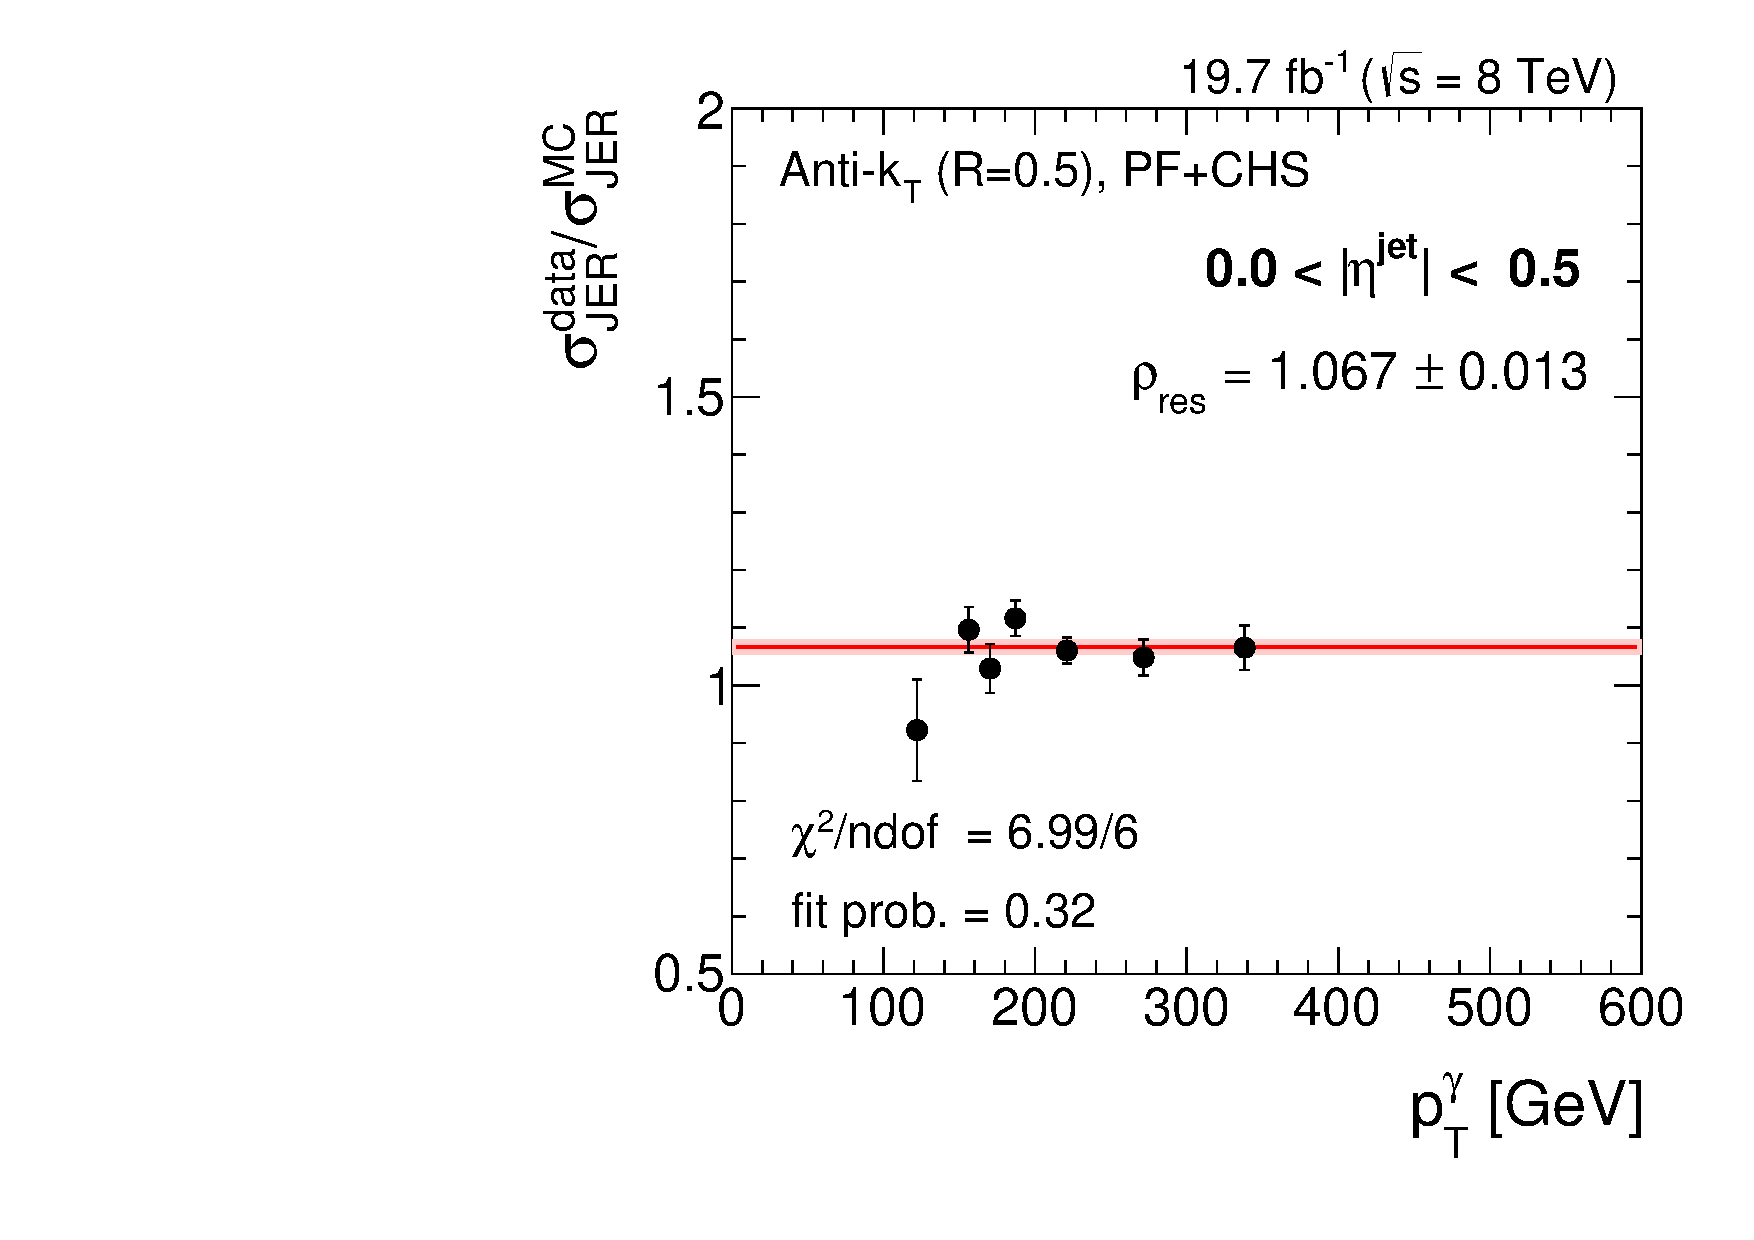
\includegraphics[width=0.49\textwidth]{figures/resolution/results/Ratio_Resolution_for_1_eta_bin_PFCHS_data_comparison_RMS99.pdf}
    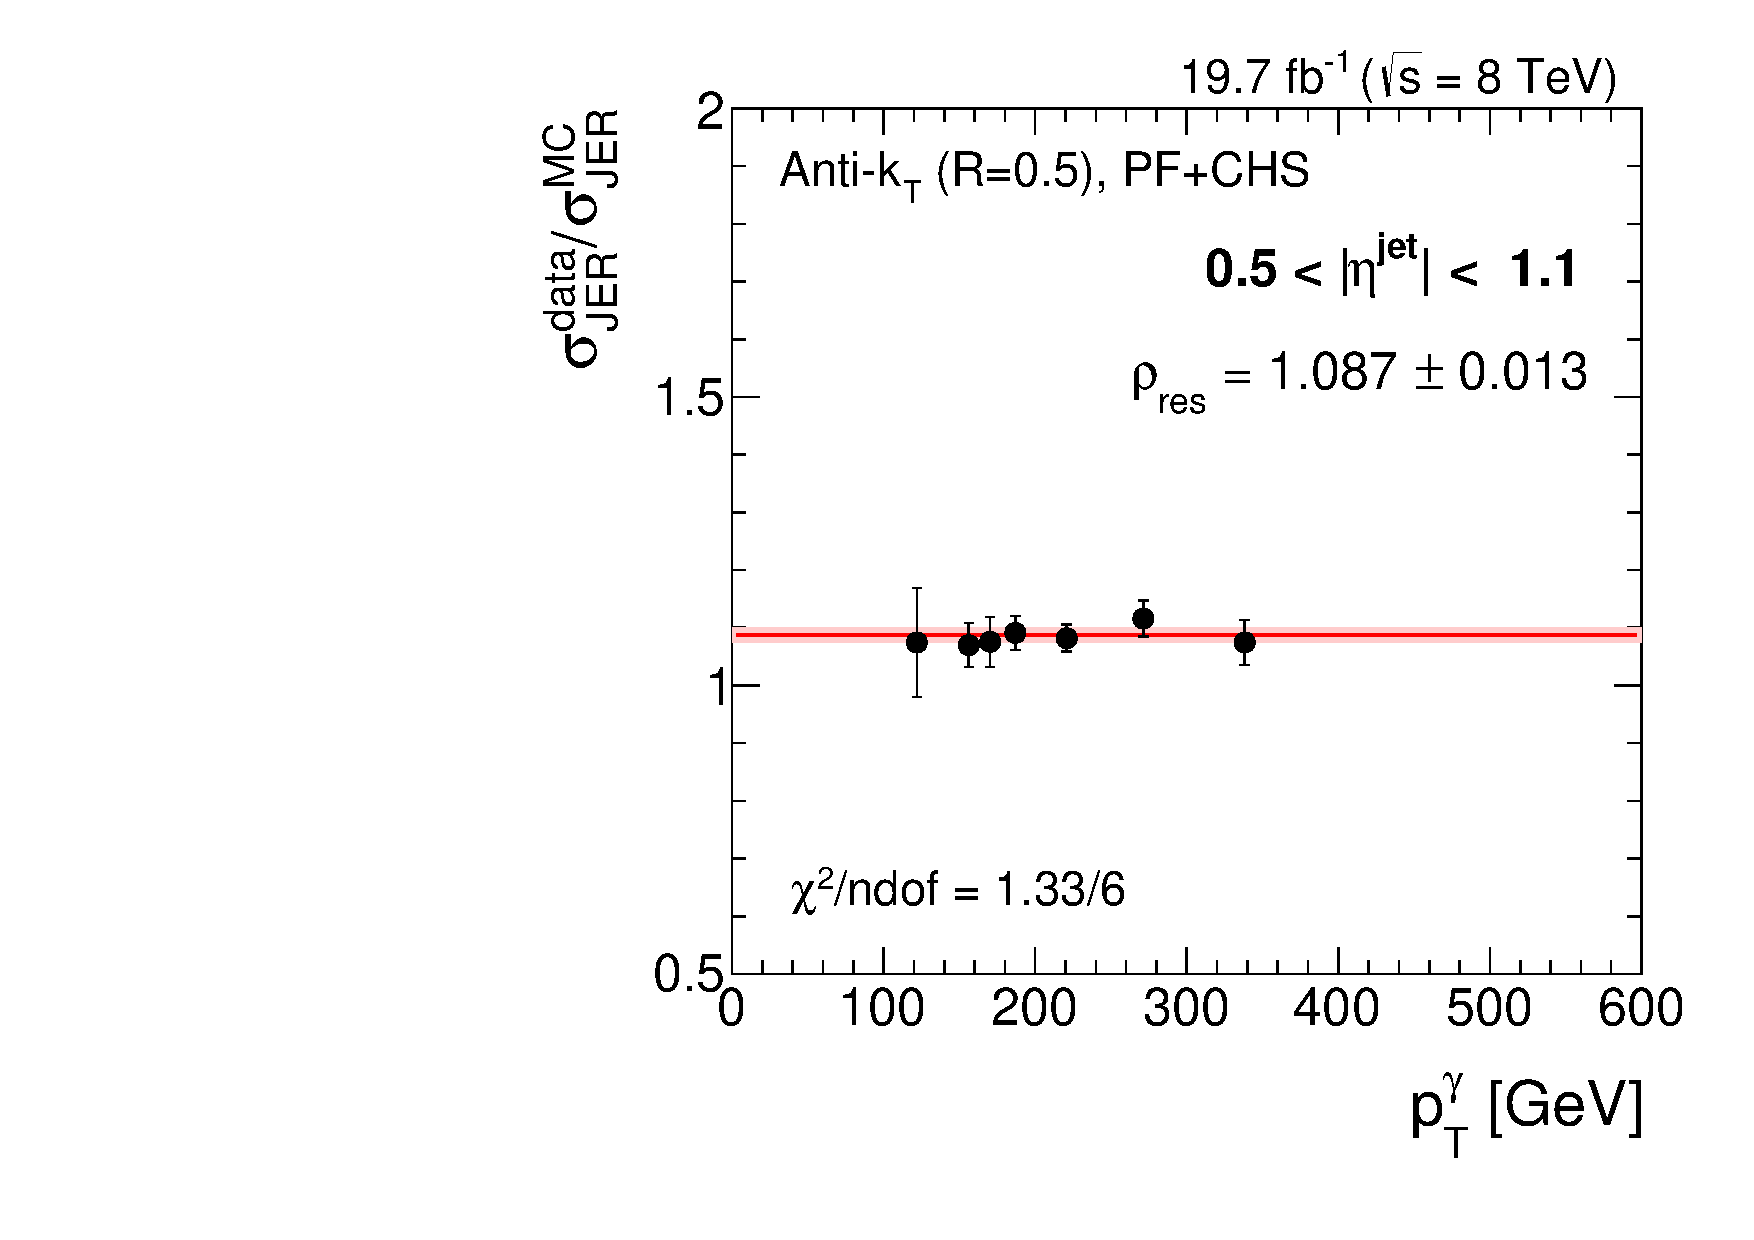
\includegraphics[width=0.49\textwidth]{figures/resolution/results/Ratio_Resolution_for_2_eta_bin_PFCHS_data_comparison_RMS99.pdf}
    \vspace{18pt}

    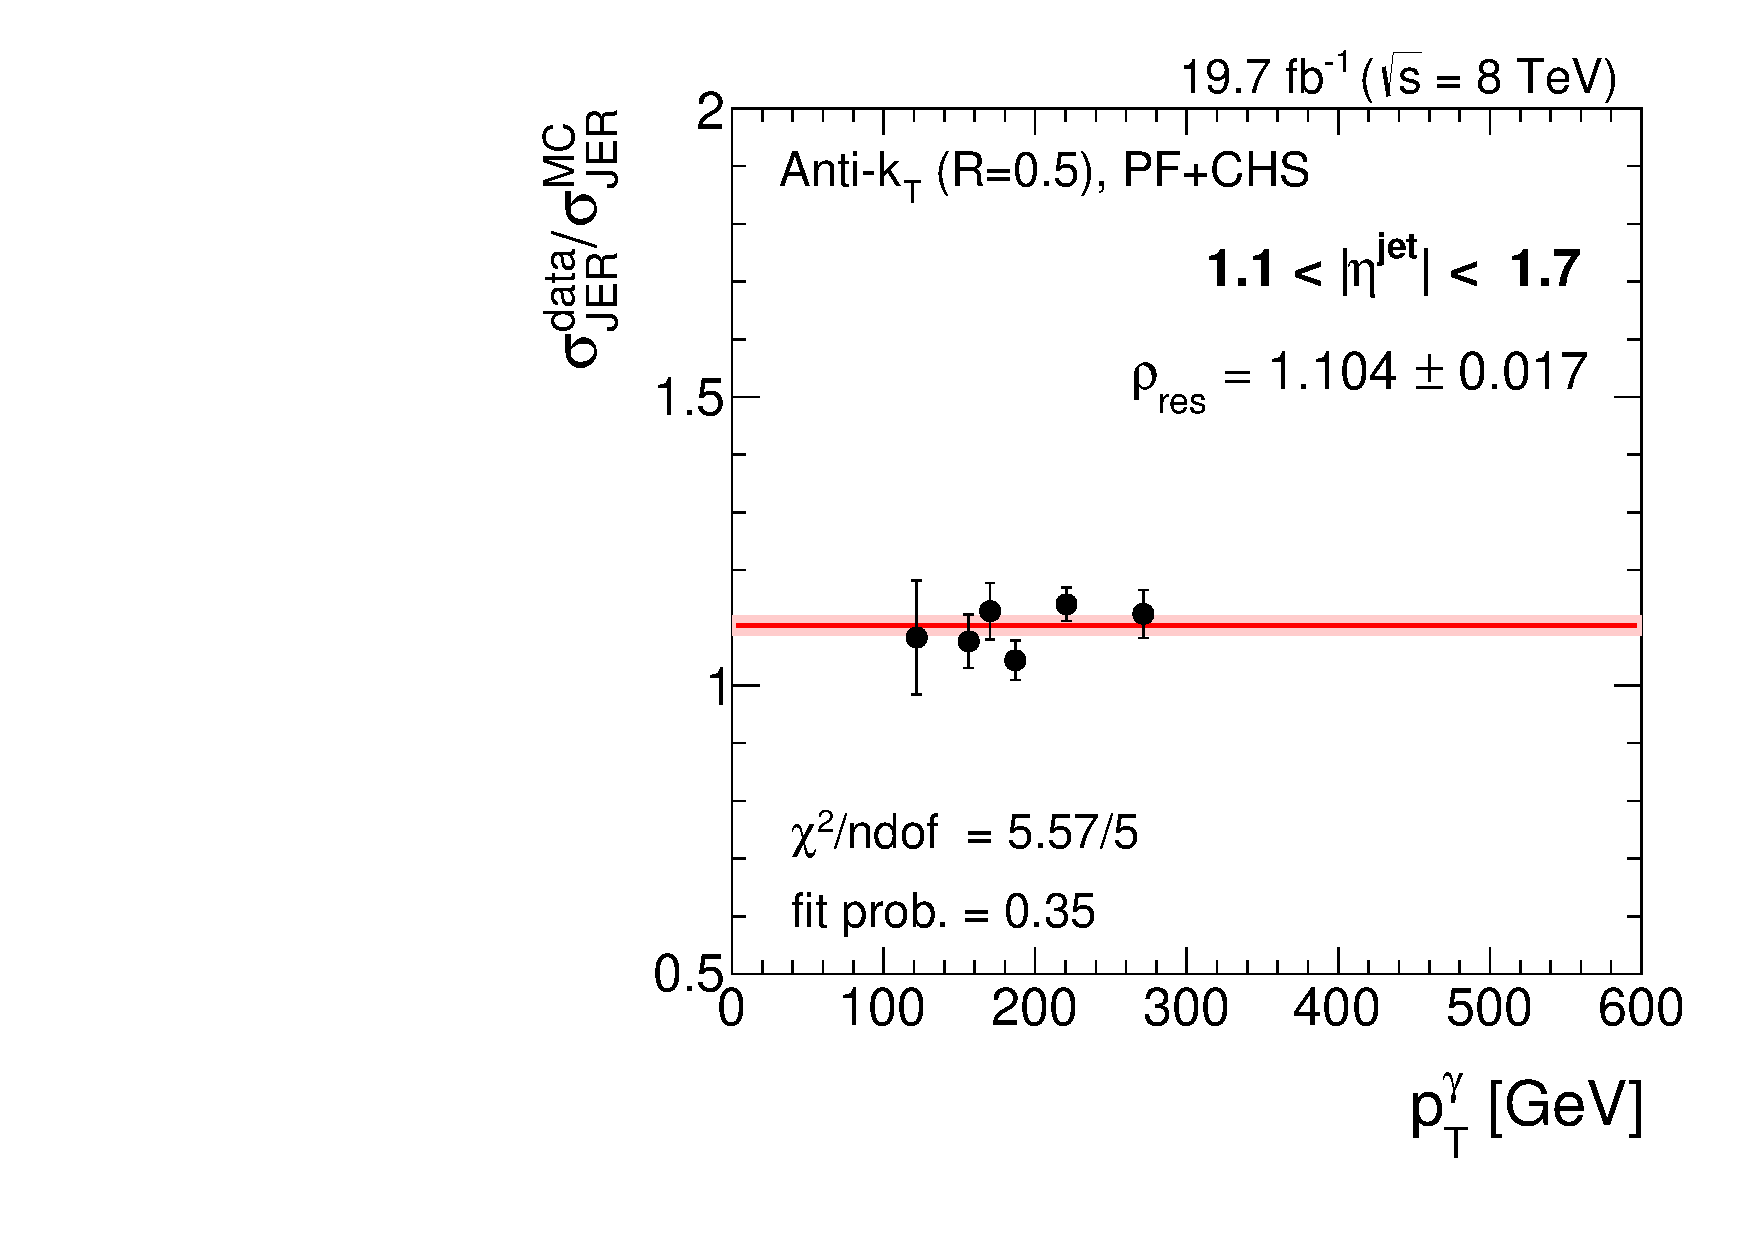
\includegraphics[width=0.49\textwidth]{figures/resolution/results/Ratio_Resolution_for_3_eta_bin_PFCHS_data_comparison_RMS99.pdf}
    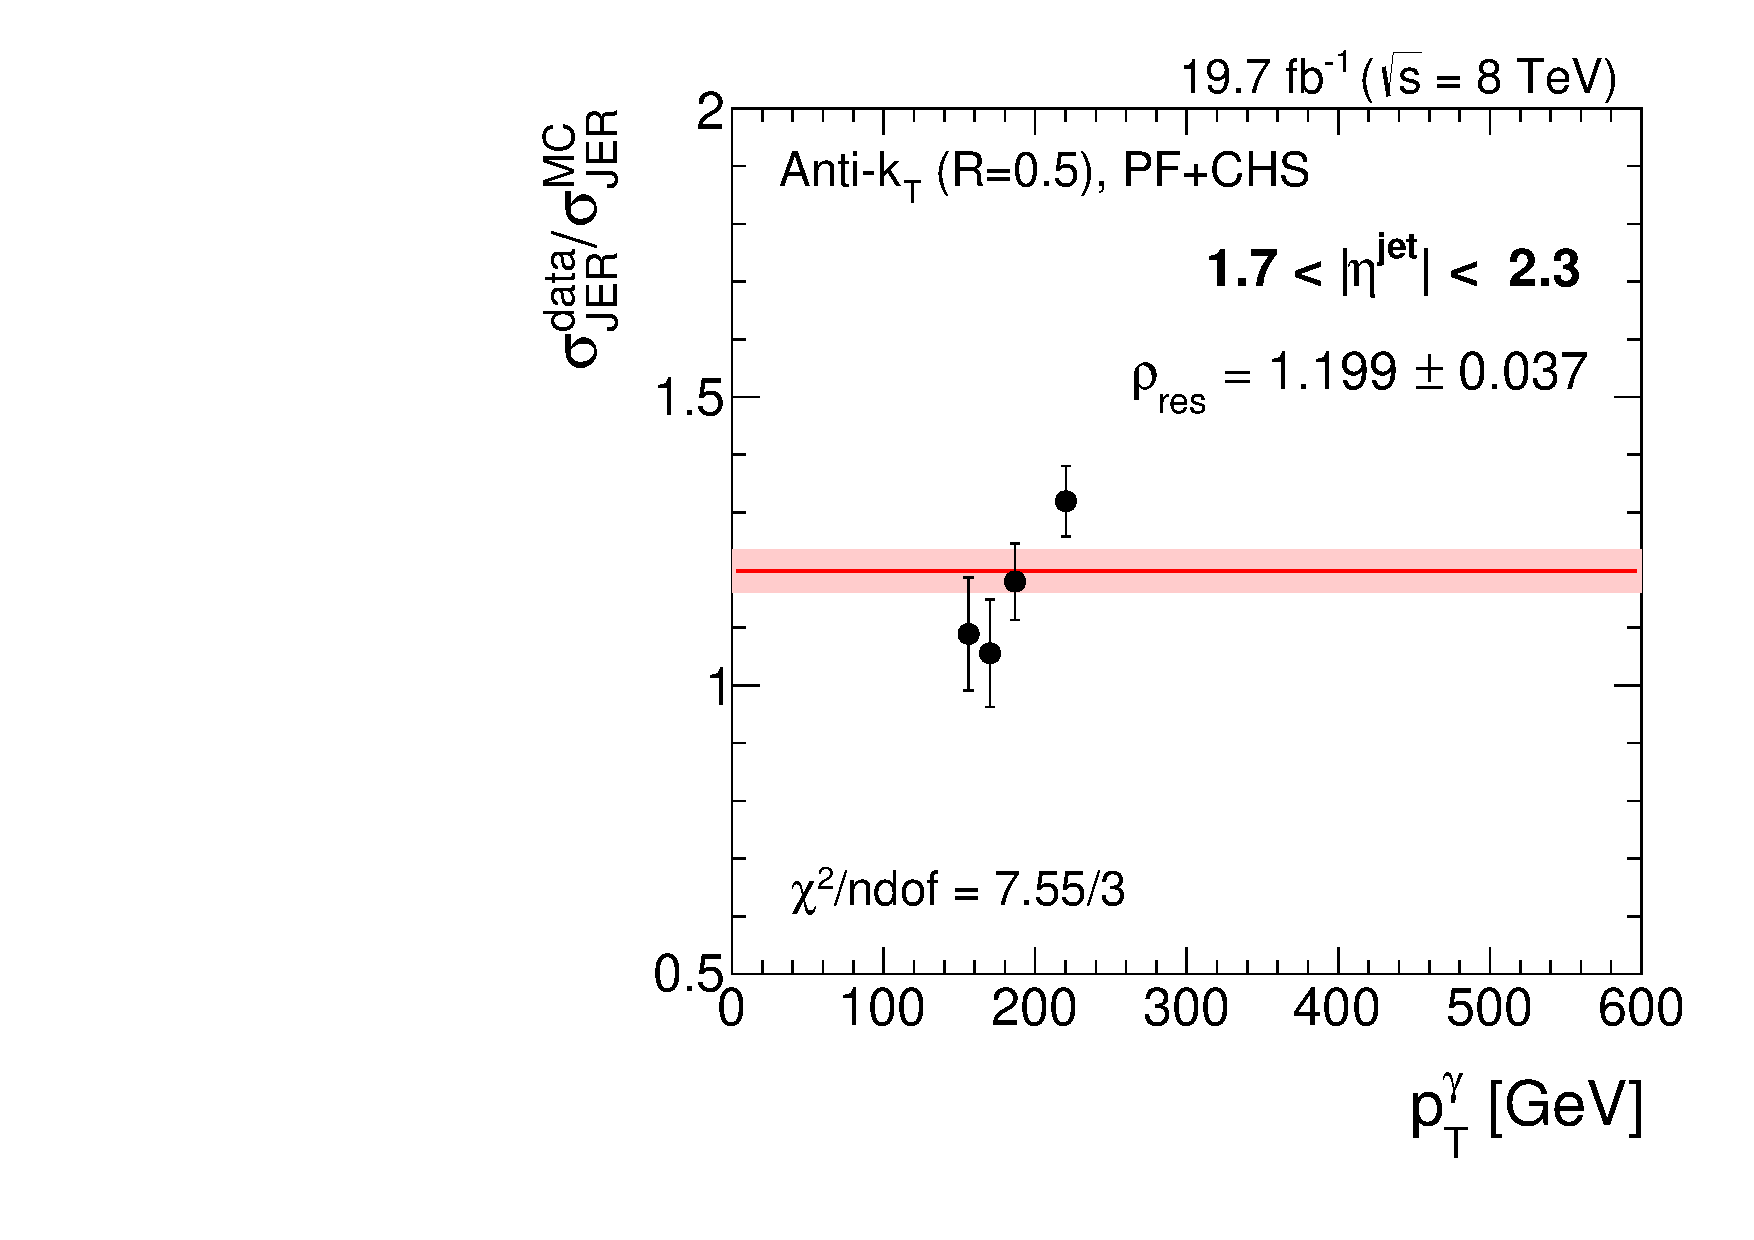
\includegraphics[width=0.49\textwidth]{figures/resolution/results/Ratio_Resolution_for_4_eta_bin_PFCHS_data_comparison_RMS99.pdf}
  \caption{Data-to-simulation resolution ratios \rhores (black dots), fitted with a horizontal line (red line) for four different $|\etajet|$-ranges.
           The fit uncertainties are depicted with light red error bands.}
  \label{res:fig:RatioEtaBinned}
\end{figure}

The resulting \rhores is always larger than one which means that the resolution in data is always worse than the resolution in simulation.
The values of the fits range from 1.067 (for the first $\etajet$-bin) to 1.199 (for the last $\etajet$-bin). 

The systematic uncertainties are evaluated as described in the previous chapter. 
The single uncertainties are taken as upper and lower boundary of the 68\% uncertainty band and are added in quadrature to get the total systematic uncertainty.
Table~\ref{res:tab:FinalResults} summarises the data-to-simulation ratio results determined with data collected during the year 2012 with their statistical and systematic uncertainties.
\renewcommand{\arraystretch}{1.5}
\begin{table}[t]
\centering
\caption{Data-to-simulation resolution scale factors \rhores with statistical and systematic uncertainties.}
\label{res:tab:FinalResults}
\large{
\makebox[0.99\textwidth]{
\begin{tabular}{  c | c   c c }
\multicolumn{4}{c}{} \\
\toprule
$|\etajet|$ & \rhores &  stat.      & sys.  \\
\midrule
$0.0 - 0.5$ &1.067 & $\pm 0.013$ & $^{+0.025}_{-0.024}$ \\
$0.5 - 1.1$ &1.087 & $\pm 0.013$ & $^{+0.039}_{-0.039}$ \\
$1.1 - 1.7$ &1.104 & $\pm 0.017$ & $^{+0.049}_{-0.049}$ \\
$1.7 - 2.3$ &1.199 & $\pm 0.037$ & $^{+0.075}_{-0.075}$ \\
\bottomrule
\multicolumn{4}{c}{} \\
\end{tabular}}}
\end{table}  
The visualised result can be found in Fig.~\ref{res:fig:RatioFinal}.\\

Though the \GAMJET analysis is known for producing highly precise results, the systematic uncertainties are still dominating. 
This is mainly caused by the uncertainty on the simulation of out-of-cone showering.
The statistical limitation of this analysis is due to the collected data at the CMS detector.
The number of simulated events is roughly eight times larger.

 
\section{Comparison to 2011 measurement}
\label{res:sec:comparison_2010}
A comparison of the data-to-simulation resolution scale factors \rhores between this analysis and the results of 2011 which were determined from a dijet data sample~\cite{bib:Matthias_Thesis} can be found in Fig.~\ref{res:fig:Comparison_2011}.
\begin{figure}[!t]
 \centering
    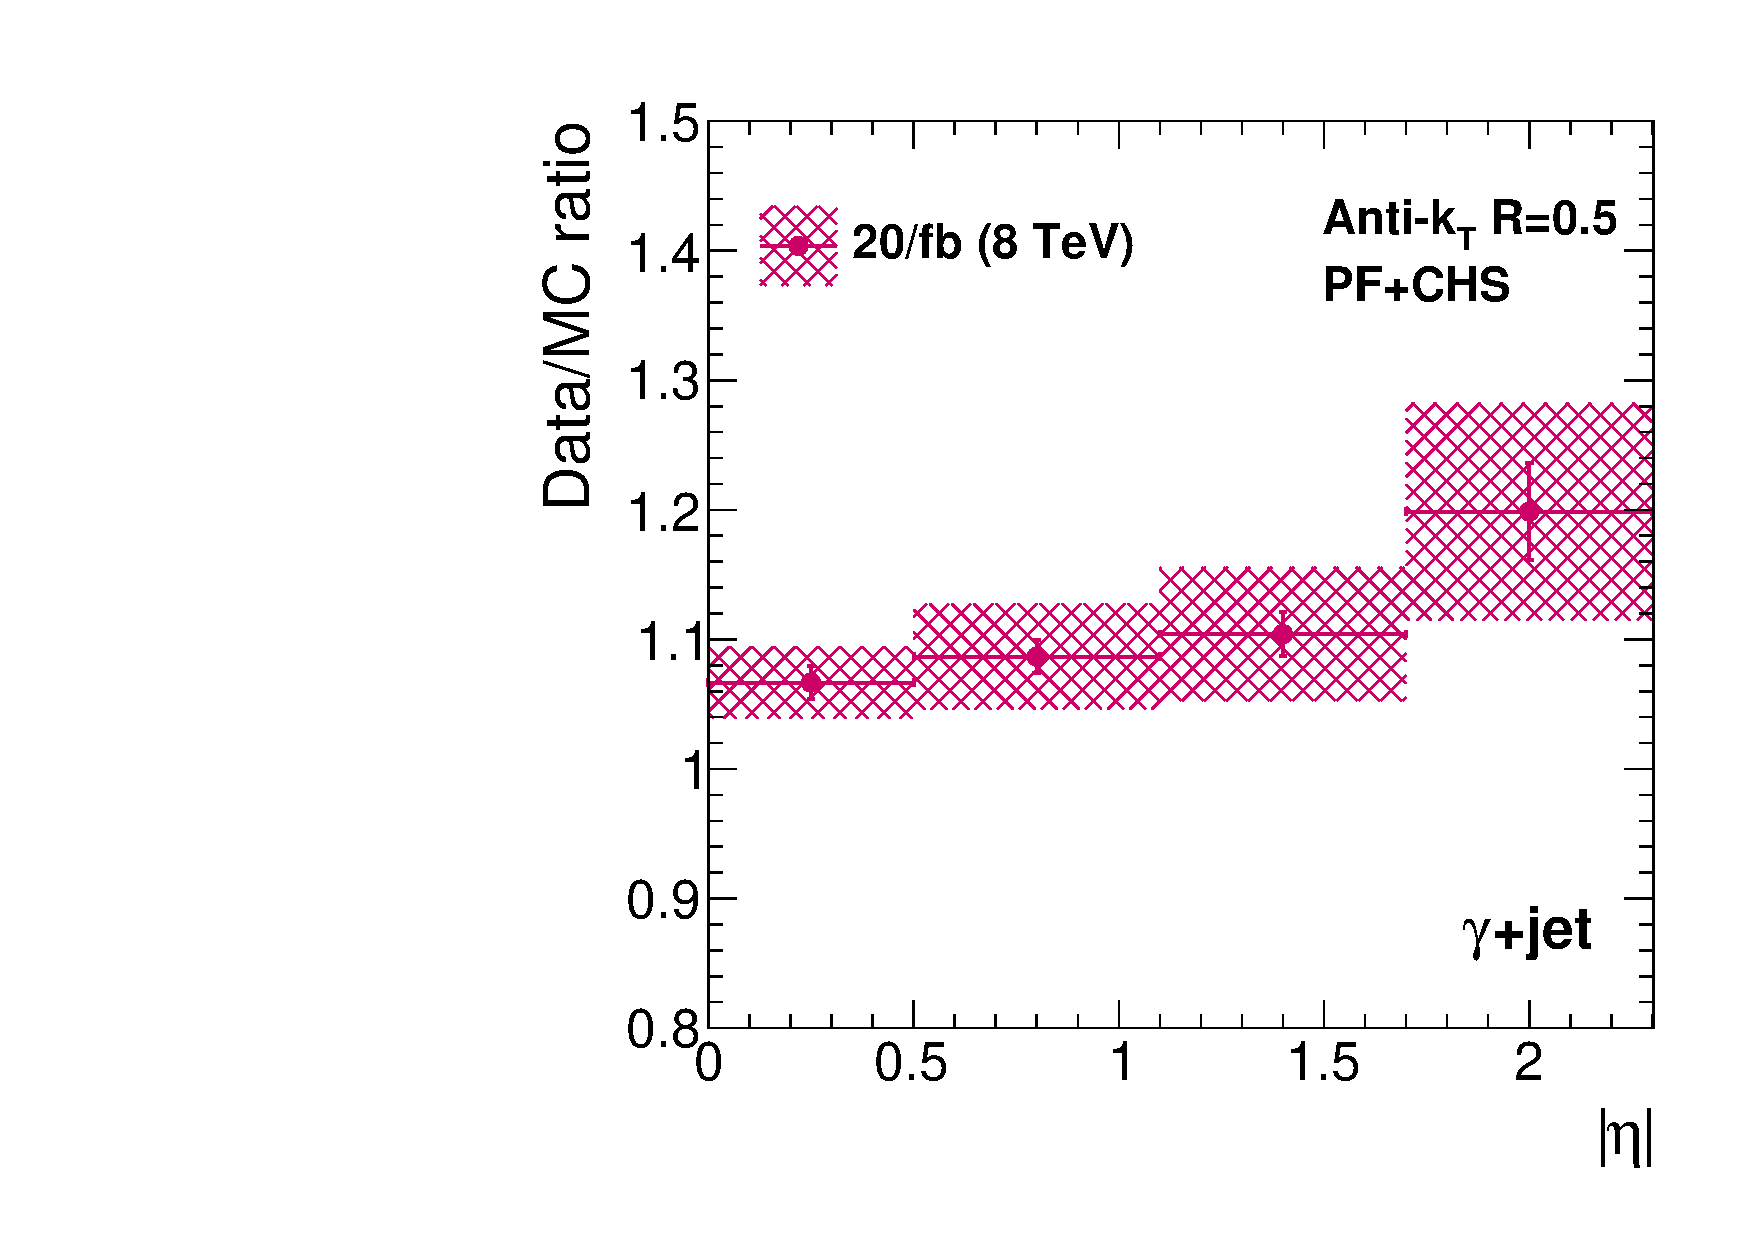
\includegraphics[width=0.54\textwidth]{figures/resolution/results/MySingleFinalResult.pdf}
  \caption{FIXME (Update this plot): The measured data-to-simulation resolution ratio in \GAMJET events using data recorded in the year 2012.
           The red band depicts the total uncertainty whereas the error bars show the statistical uncertainty only.}
  \label{res:fig:RatioFinal}
\end{figure}
\begin{figure}[!t]
 \centering
    %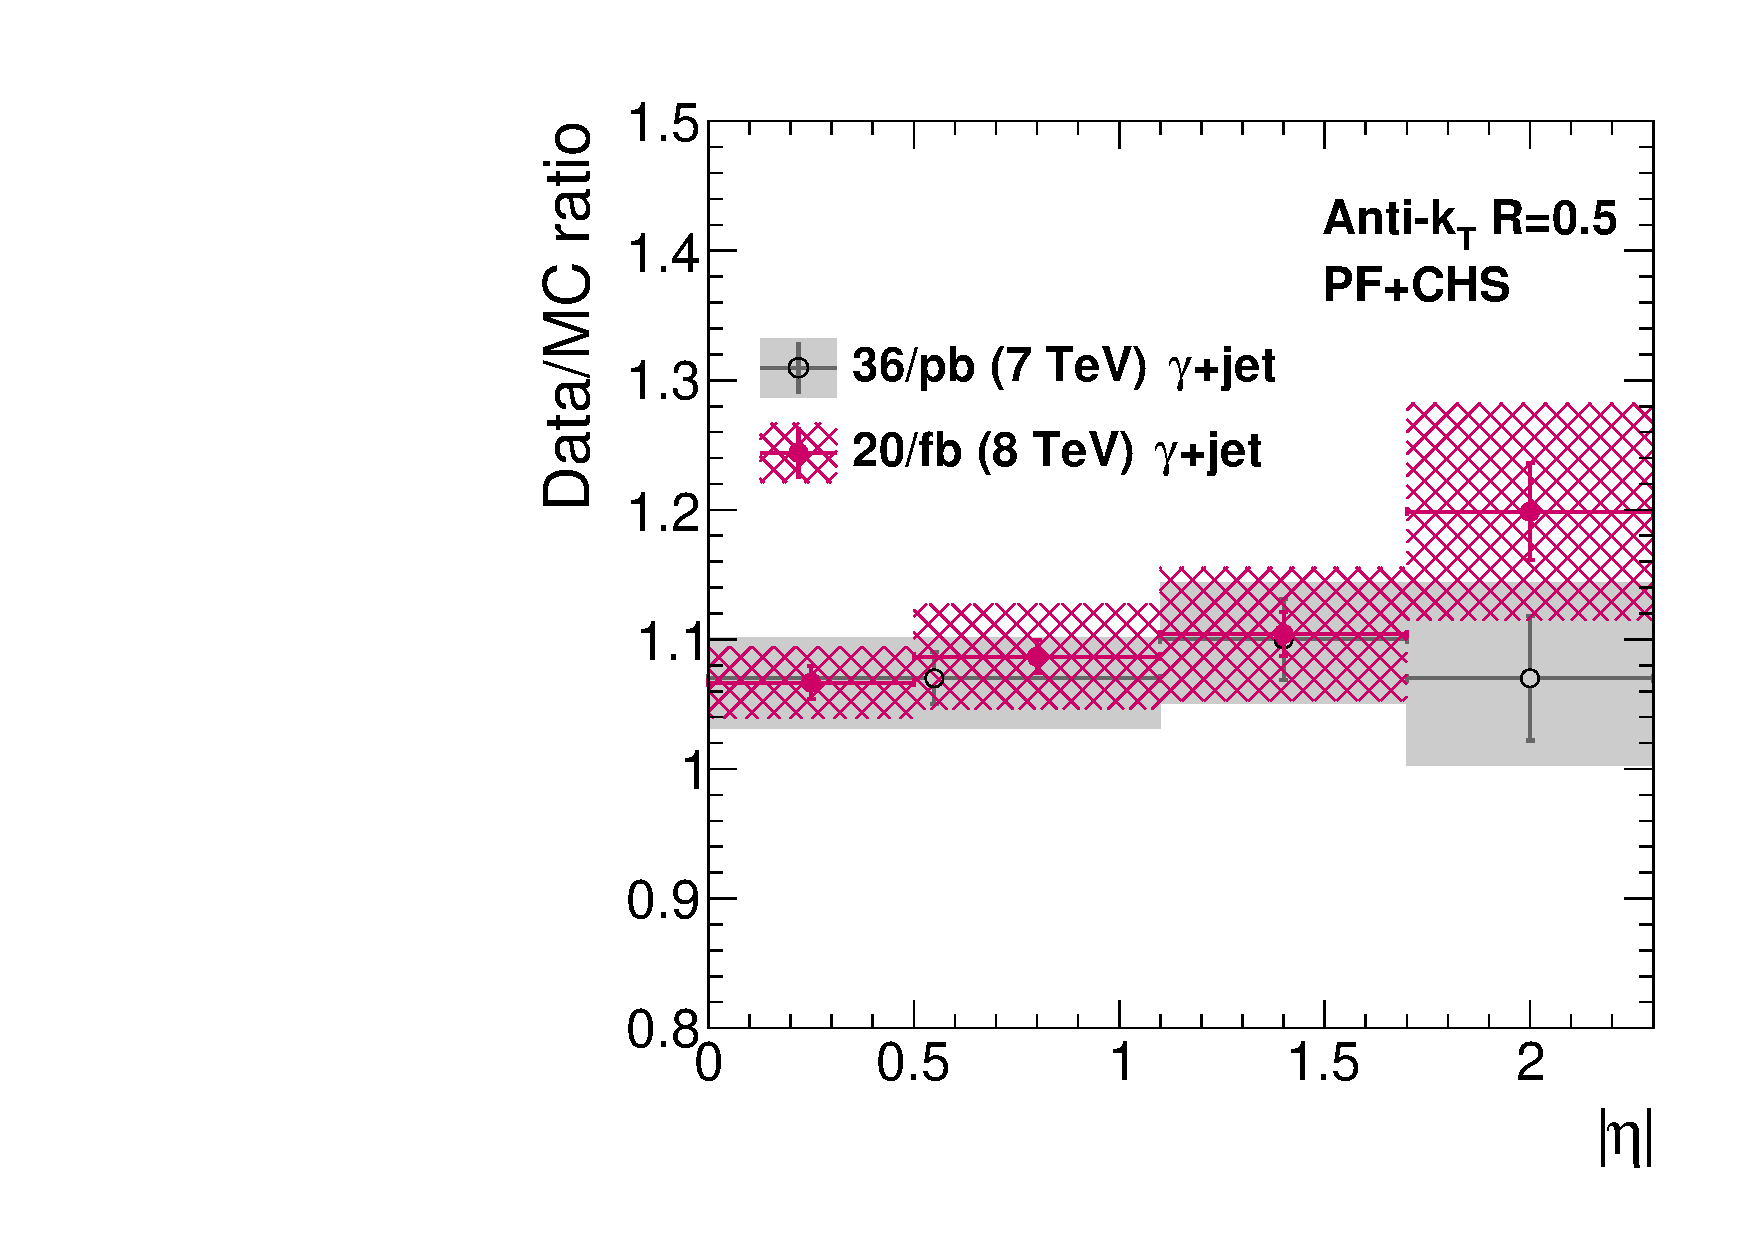
\includegraphics[width=0.65\textwidth]{figures/resolution/results/ComparisonTo2012_GAMJET.pdf}
    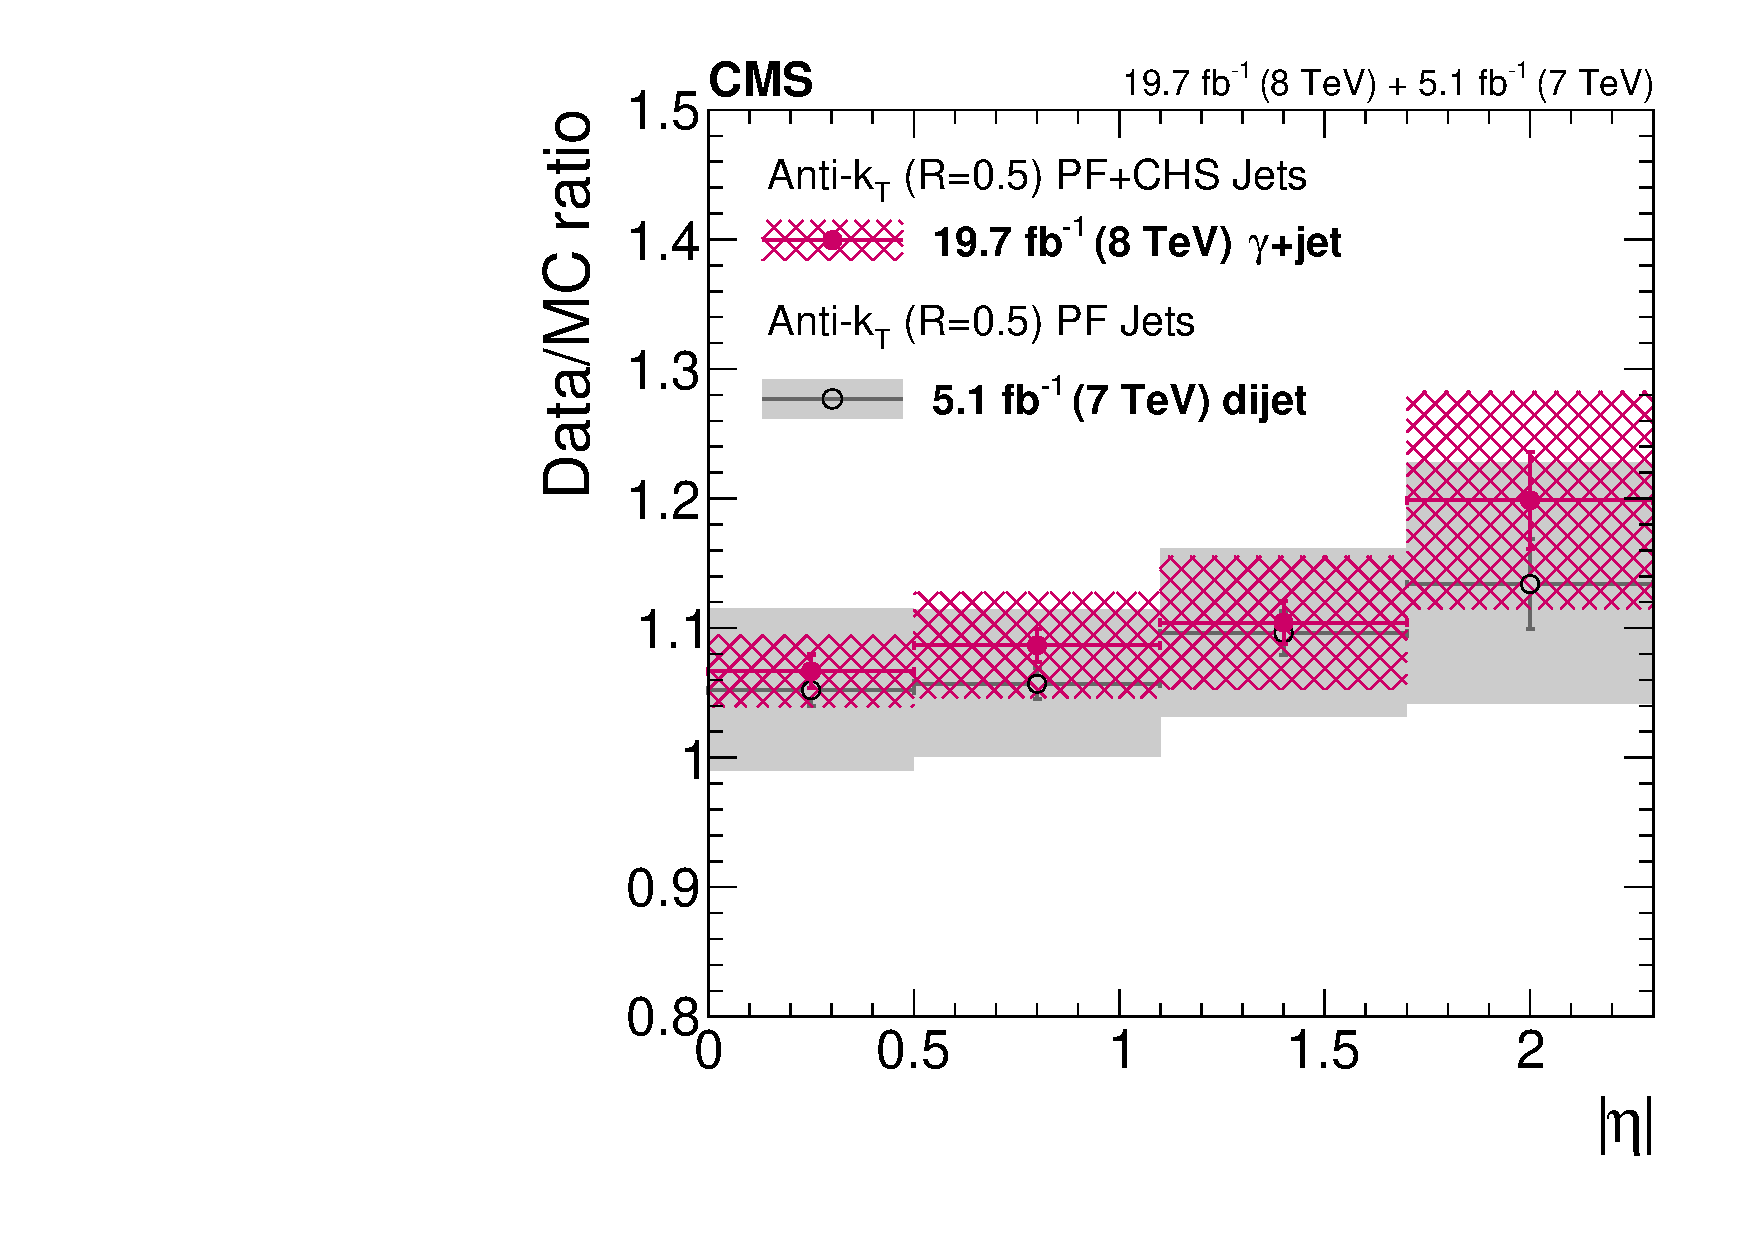
\includegraphics[width=0.54\textwidth]{figures/resolution/results/Figure_43_left_Teresa_cmsStyle_updated_5.pdf}
  \caption{FIXME (update this plot): Data-to-simulation jet-\pt resolution ratio determined from \GAMJET events from 2012 compared to dijet results from 2011.
           The grey and magenta bands correspond to the full uncertainties, whereas the error bars depict the statistical uncertainties only.}
  \label{res:fig:Comparison_2011}
\end{figure}
It can be seen, that throughout the whole \etajet-range the data-to-simulation resolution ratios \rhores are systematically larger for the result in 2011. 
Comparing the precision of both measurements, the \GAMJET analysis is for all $\eta$-bins more precise than the analysis done with dijet events.
This is due to the smaller systematic uncertainties of this analysis which compensates for the better statistical precision of the QCD-multijet sample due to the large cross section.


\section{Comparison to 2012 dijet measurement}
\label{res:sec:comparison_2012}
A jet-\pt resolution measurement using dijet events was also carried out in 2012~\cite{bib:CMS:JME_PAS,bib:Kristin_Thesis}.
A comparison of the here presented measurement using \GAMJET events to the measurement with dijet events can be found in Fig.~\ref{res:fig:Comparison_2012}.
\begin{figure}[!t]
 \centering
    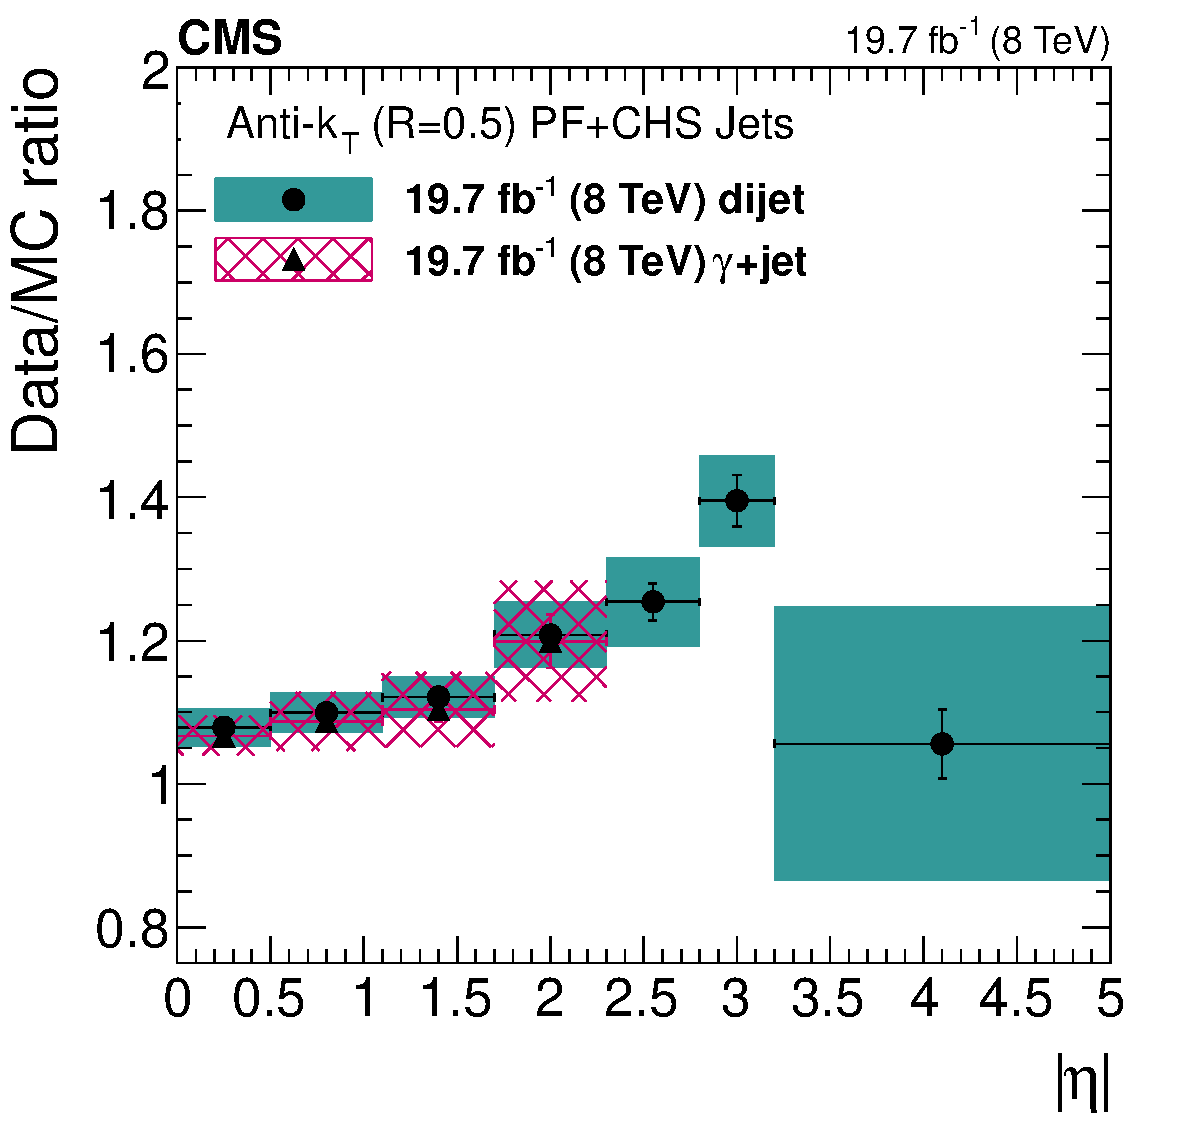
\includegraphics[width=0.55\textwidth]{figures/resolution/results/JER_2012_compPhoton_final_v2.pdf}
  \caption{FIXME (Update this plot): Data-to-simulation jet-\pt resolution ratio determined from \GAMJET events from 2012 compared to dijet results from 2012.
           The blue and magenta bands correspond to the full uncertainties, whereas the error bars depict the statistical uncertainties only.}
  \label{res:fig:Comparison_2012}
\end{figure}
Both measurements are compatible within their uncertainties.
It can be seen that the statistical precision is much better for the measurement with QCD-multijet events because of the larger cross section.
The systematic uncertainties are of comparable size for small pseudorapidity bins and are larger for high $|\etajet|$ in the here presented measurement.
This is due to the uncertainty on the simulation of the out-of-cone showering.
This uncertainty plays a smaller role in the dijet measurement (between 0.4\% and 1.5\%) as the effect by out-of-cone showering partly cancels out in case of two balanced jets.
%Also, the different evaluation in the two measurements influences the size of this uncertainty.
%In the dijet measurement this uncertainty was evaluated by varying the residual imbalance by $\pm$25\%.
%Such an evaluation would result in smaller uncertainties for the large pseudorapidity region in the \GAMJET measurement.
%%%%%%%%%%%%%%%%%%%%%%%%%%%%%%%%%%%%%%%%%%%%%%%%%%%%%%%%%%%%%%%%%%%%%%%%%%%%%%%%%%%%%%%%%%%%%%%%%%%%%%%%%%%%%%%%%%%%%%%%%%%%%%%%%%%%%%%%%%%%%%%%%%%%%%%%%%%%%%%%%%%%%%%%%%%%%%%%%%%%%%%%%%%%%%%%%%%%%%%%%%%%%%%%%%%%%%%%%%%%%%%%%%%
%%%%%%%%%%%%%%%%%%%%%%%%%%%%%%%%%%%%%%%%%%%%%%%%%%%%%%%%%%%%%%%%%%%%%%%%%%%%%%%%%%%%%%%%%%%%%%%%%%%%%%%%%%%%%%%%%%%%%%%%%%%%%%%%%%%%%%%%%%%%%%%%%%%%%%%%%%%%%%%%%%%%%%%%%%%%%%%%%%%%%%%%%%%%%%%%%%%%%%%%%%%%%%%%%%%%%%%%%%%%%%%%%%%
%%%%%%%%%%%%%%%%%%%%%%%%%%%%%%%%%%%%%%%%%%%%%%%%%%%%%%%%%%%%%%%%%%%%%%%%%%%%%%%%%%%%%%%%%%%%%%%%%%%%%%%%%%%%%%%%%%%%%%%%%%%%%%%%%%%%%%%%%%%%%%%%%%%%%%%%%%%%%%%%%%%%%%%%%%%%%%%%%%%%%%%%%%%%%%%%%%%%%%%%%%%%%%%%%%%%%%%%%%%%%%%%%%%
\FloatBarrier
\chapter{Discussion and conclusion}
The difference of the jet transverse-momentum resolution between data and simulation is an important input for many analyses at CMS, including searches for physics beyond the Standard Model using QCD-multijet events, \eg\cite{bib:CMS:RA2_8TeV,bib:CMS:MT2_8TeV,bib:CMS:AlphaT_8TeV}.

In this analysis, the first measurement of the data-to-simulation scale factors \rhores %resolution ratio $\jer^{\text{data}}/\jer^{\text{MC}}$ 
using \GAMJET events with $19.7\fbinv$ $pp$-collision data at $\sqrt{s}=8 \tev$ collected in 2012 at the CMS detector is presented.
The analysis relies on the methodology developed in~\cite{bib:CMS:JERCPaper_2011,CMS:PAS:JETResolution_7TeV}.
During the study, it was found that the jet transverse-momentum response depends on the topology of additional jet activity in the events, leading to a double peak structure.
This was not accounted for in previous analyses~\cite{bib:CMS:JERCPaper_2011,CMS:PAS:JETResolution_7TeV}.
Therefore, a new method has been developed within this thesis to consistently deal with the distortion of the response distribution due to additional jets from initial and final state radiation (see Section~\ref{res:ch:methodology}).\\
%take account of the double peak structure when applying an exclusive binning in the variable $\alpha$ which measures the additional jet activity in the event, the event selection explicitly distinguishes the case of parton radiation in the leading jet/photon hemispheres.
%This change in methodology is introduced for the first time by this measurement.\\

The resolution in data is found to be systematically larger than in simulation by around $7\%$ to $20\%$ throughout the investigated \etajet plane. 
A possible \ptjet dependence of the resolution scale factors \rhores is not visible. 
Thus, the ratio is parametrised with a constant for each \etajet-bin.
The accuracy of the measurement is dominated by systematic uncertainties, leading to a total uncertainty of 3\% to 8\%.
The results of this analysis compare well to similar studies, including a dijet study at 8\tev ~\cite{bib:CMS:JME_PAS,bib:Kristin_Thesis}.
Both measurements are compatible within their statistical and systematic uncertainties.\\

For a future measurement, a reduction of the uncertainties is desirable.
The main source of uncertainty is the systematic uncertainty on the simulation of out-of-cone showering.
Within this analysis, this uncertainty was estimated by varying the jet clustering radius from R=0.5 to R=0.7.
This approach might be conservative, since the difference in \rhores associated with different jet clustering radii may include other effects than out-of-cone showering.
Thus, a more detailed investigation of the quality of out-of-cone showering simulation could yield a reduced uncertainty of the \rhores measurement using \GAMJET events.

Furthermore, an increase in the statistical precision is desirable to allow for the determination of resolution scale factors in the high pseudorapidity regions which have not been accessible so far.
%Since the systematic uncertainty is dominating, most notably the uncertainty on the simulation of out-of-cone showering, an improved evaluation of the out-of-cone showering uncertainty could significantly improve the precision of the data-to-simulation ratio $\jer^{\text{data}}/\jer^{\text{MC}}$.
%A better evaluation can possibly be achieved by a better understanding, whether the difference of \rhores using clustered jets within a radius of 0.7 and 0.5 is only originating from out-of-cone showering effects.
%Since the simulation of out-of-cone showering should in principal only enter the result by the residual imbalance $q$, an overestimation by the here presented method might be possible.



%The significant advantage of a jet-\pt resolution measurement using \GAMJET events over a measurement with dijet events is the absolute reference \pt measured with a reconstructed photon.
%This allows the exclusive binning in alpha 


